\chapter{Model 1: Dirac and Weyl Semimetals}\label{chap:Model1}

\section{Introduction}\label{sec:introduction}
Dirac and Weyl semimetals are nodal electronic phases of matter in three spatial dimensions. Their low-energy emergent quasiparticle excitations are electronic Dirac~\cite{Dirac28} and Weyl~\cite{Weyl29} fermions. (Contemporary reviews in condensed electronic matter can be found in Ref.~\cite{Ashvin_Weyl_review,TurnerVishwanath13,HasanXuBian15,RMP,Burkov16,JiaXuHasan16,ArmitageMeleVishwanath16,YanFelser17}.) They are three dimensional generalizations of the Dirac fermions that appear in two dimensional graphene~\cite{NetoGuineaPeresNovoselovGeim09} and the surface boundary of a topological insulator~\cite{HasanKane10,QiZhangreview11,HasanMoore11,RMP}. They follow massless quasi-relativistic linear dispersions near nodal points in the energy-momentum space close to the Fermi level. Contrary to accidental degeneracies which can be lifted by generic perturbations, these nodal points are protected by topologies or symmetries. 

A Weyl fermion is {\em chiral} and has a non-trivial winding of a pseudo-spin texture near the singular nodal point in energy-momentum space. This would associate to a non-conservative charge current under a parallel electric and magnetic field and is known as the Adler-Bell-Jackiw (\hypertarget{ABJ}{ABJ}) anomaly~\cite{Adler69,BellJackiw69}. Thus, in a true three dimensional lattice system, Weyl fermions must come in pairs~\cite{Nielsen_Ninomiya_1981,NielsenNinomiyaPLB1981,NielsenNinomiya83} so that the net chirality, and consequently the anomaly, cancels. Or otherwise, a three dimensional system of a single Weyl fermion must be holographically supported as the boundary of a topological insulator in four dimensions~\cite{ZhangHu01,BernevigChernHuToumbasZhang02,QiHughesZhang08}. On the other hand, a Dirac fermion in three dimensions consists of a pair of Weyl fermions with opposite chiralities. Without symmetries, it is not stable and can turn massive upon inter-Weyl-species coupling. With symmetries, a band crossing can be protected by the distinct symmetry quantum numbers the bands carry along a high symmetry axis. In this article, we focus on the fourfold degenerate Dirac nodal point protected by time-reversal (\hypertarget{TR}{TR}) and (screw) rotation symmetry.

In electronic systems, massless Dirac and Weyl fermions appear in gap-closing phase transitions between spin-orbit coupled topological insulators and normal insulators~\cite{Murakami2007}. When inversion or time-reversal symmetry is broken, nodal Weyl points can be separated in energy-momentum space. Such gapless electronic phases are contemporarily referred to as Weyl (semi)metals~\cite{WanVishwanathSavrasovPRB11,YangLuRan11,burkovBalenstPRL11,BurkovBalentsPRB11}. Their boundary surfaces support open Fermi arcs~\cite{WanVishwanathSavrasovPRB11} that connect surface-projected Weyl nodes. Weyl (semi)metals also exhibit exotic transport properties, such as negative magneto-resistance, non-local transport, chiral magnetic effect, and chiral vortical effect~\cite{Burkov_Weyl_electromagnetic_2012,Hosur_Weyl_develop,Lu_anomaly_Weyl_2013,SonSpivak13,Sid_anomaly_Weyl,Marcel_Weyl_response}. There have been numerous first principle calculations~\cite{WengXiZhong16} on proposed materials such as the non-centrosymmetric (La/Lu)Bi$_{1-x}$Sb$_x$Te$_3$~\cite{LiuVanderbilt14}, the TlBiSe$_2$ family~\cite{SinghSharmaLinHasanPrasadBansil12}, the TaAs family~\cite{WengBernevigDai2015,HuangXuZahidTaAs2015}, trigonal Se/Te~\cite{HirayamaOkugawaIshibashiMurakamiMiyake15} and the HgTe class~\cite{RuanXing16}, as well as the time-reversal breaking pyrochlore iridates \cite{WanVishwanathSavrasovPRB11,witczak_kim_weyl_2012,chen_hermele_weyl}, magnetically doped topological and trivial insulator multilayers \cite{burkovBalenstPRL11}, HgCr$_2$Se$_4$~\cite{XuWengWangDaiFang11} and Hg$_{1-x-y}$Cd$_x$Mn$_y$Te~\cite{BulmashLiuQi14}. At the same time, there have also been abundant experimental observations in bulk and surface energy spectra~\cite{HasanXuBelopolskiHuang17} as well as transport~\cite{WangLinWangYuLiao17}. Angle-resolved photoemission spectroscopy (\hypertarget{ARPES}{ARPES}) showed bulk Weyl spectra and surface Fermi arcs in TaAs~\cite{Xu_Weyl_2015_first,Weyl_discovery_TaAs,YangLiuChenTaAs2015,TaAs_Weyl_obeservationDing,BelopolskiZahid16} as well as similar materials such as NbAs, NbP and TaP~\cite{XuNbAs15,LiuChen16}. Other materials such as Ag$_3$BO$_3$, TlTe$_2$O$_6$ and Ag$_2$Se~\cite{ChangHasan16} were observed to host pinned Weyl nodes at high symmetry points. %theory pinned along screw axis {TsirkinSouzaVanderbilt17}
Negative magneto-resistance was reported in TaAs~\cite{Huang_Weyl_2015,Zhang_anomaly_Weyl_2015} as a suggestive signature of the \ABJ anomaly. Similar properties were also observed in TaP~\cite{HuMaoTaP17}, NbP and NbAs~\cite{CorinnaNiemannFelserNbP17,LiXuNbAsNbP17,GoothNielschNbP17}, although not without controversies~\cite{SudeshPatnaikNbP17}. 

Weyl points with opposite chiralities cannot be separated in energy-momentum space when both inversion and time reversal symmetries are present. Massless Dirac fermions appear between gap-closing phase transitions between topological and trivial (crystalline) insulators, such as Bi$_{1-x}$Sb$_x$~\cite{TeoFuKane08} and Pb$_{1-x}$Sn$_x$Te~\cite{Hsieh:2012fk}. Critical Dirac (semi)metals were investigated for example in the tunable TlBiSe$_{2-x}$S$_x$~\cite{SatoTakahashi11,SoumaAndo12,XuCavaHasan11}, Bi$_{2−x}$In$_x$Se$_3$~\cite{BrahlekSeongshik12,WuArmitage13} and Hg$_{1-x}$Cd$_x$Te~\cite{OrlitaPotemski14}, as well as the charge balanced BaAgBi~\cite{DuWanXYBi15}, PtBi$_2$, SrSn$_2$As$_2$~\cite{GibsonCava15} and ZrTe$_5$~\cite{LiVallaZrTe516} whose natural states are believed to be close to a topological critical transition. A Dirac (semi)metallic phase can be stabilized when the Dirac band crossing is secured along a high symmetry axis and the two crossing bands carry distinct irreducible representations. Theoretical studies include the diamond-structured $\beta$-crystobalite BiO$_2$ family~\cite{BiO3_Dirac_semimetal} (space group (\hypertarget{SG}{SG}) No.~227, Fd3m), the orthorhombic body-centered BiZnSiO$_4$ family~\cite{SteinbergYoungZaheerKaneMeleRappe14} (\SG No.~74, Imma), the tetragonal Cd$_3$As$_2$~\cite{wangCd3As2PRB13} (\SG No.~142, I4$_1$/acd), the hexagonal Na$_3$Bi family~\cite{Dai_predition_Na3Bi}, as well as the filling-enforced non-symmorphic Dirac semimetals~\cite{KonigMermin97,ParameswaranTurnerArovasVishwanath13,WatanabePoVishwanathZaletel15,ChenKimKee16,WatanabePoZaletelVishwanath16,BradlynBernevig17} such as the hexagonal TlMo$_3$Te$_3$ family~\cite{GibsonCava15} (\SG No.~176, P6$_3$/m), the monoclinic Ca$_2$Pt$_2$Ga (\SG No.~15, C2/c), AgF$_2$, Ca$_2$InOsO$_6$ (\SG No.~14, P2$_1$/n), and the orthorhombic CsHg$_2$ (\SG No.~74, Imma)~\cite{ChenPoNeatonVishwanath16}. At the same time, there are numerous experimental confirmations. They include \ARPES observations on Cd$_2$As$_3$~\cite{Cd3As2Chen2014,neupaneDiracHasan,borisenkoPRLCd3As2}, Na$_3$Bi~\cite{Liu21022014,Xu18122014} and ZrTe$_5$~\cite{LiVallaZrTe516}; scanning tunneling microscopy in Cd$_2$As$_3$~\cite{Yazdani_CdAs}; magneto-transport in Bi$_{1-x}$Sb$_x$~\cite{KimLiBiSb13}, Cd$_2$As$_3$~\cite{liangOngTransportCd3As2,HeLi14,XiangChen15,FengLuCd3As215,LiYuCd3As215,LiWangCd3As216,GuoLeeCd2As316,ZhangXiuCd3As217}, Na$_3$Bi~\cite{Xu18122014,XiongOng15}, ZrTe$_5$~\cite{ZhengMingliangZrTe514,LiVallaZrTe516,LiangOngHallZrTe516,YuanXiuZrTe516}, HfTe$_5$~\cite{WangWangHfTe516} and PtBi$_2$~\cite{GaoTianPtBi217}; magneto-optics~\cite{AkrapOrlitaCd2As316} and anomalous Nernst effect~\cite{LiangOngNernstCd3As217} in Cd$_2$As$_3$, and many more. However, there are also contradicting pieces of evidence, especially in ZrTe$_5$ and HfTe$_5$ that suggest a bulk band gap~\cite{WengDaiFangZrTe514,LiXingZrTe516,WuPanZrTe516,MoreschiniGrioniZrTe516,ManzoniCrepaldiZrTe516,ManzoniParmigianiZrTe517,FanZhouZrTe517}.
%Cd3As2
%SdH\cite{HeLi14,XiangChen15,GuoLeeCd2As316} negative magnetoresistance\cite{liangOngTransportCd3As2} anomalous Nernst effect\cite{LiangOngNernstCd3As217} magneto-optics\cite{AkrapOrlitaCd2As316}
%Na3Bi
%negative magnetoresistance\cite{Xu18122014,XiongOng15}
%ZrTe5
%negative magnetoresistance\cite{ZhengMingliangZrTe514,LiVallaZrTe516} anomalous Hall\cite{LiangOngHallZrTe516}
%HfTe5
%negative magnetoresistance\cite{WangWangHfTe516}
%PtBi2
%magnetoresistance\cite{GaoTianPtBi217}

\begin{figure}[htbp]
	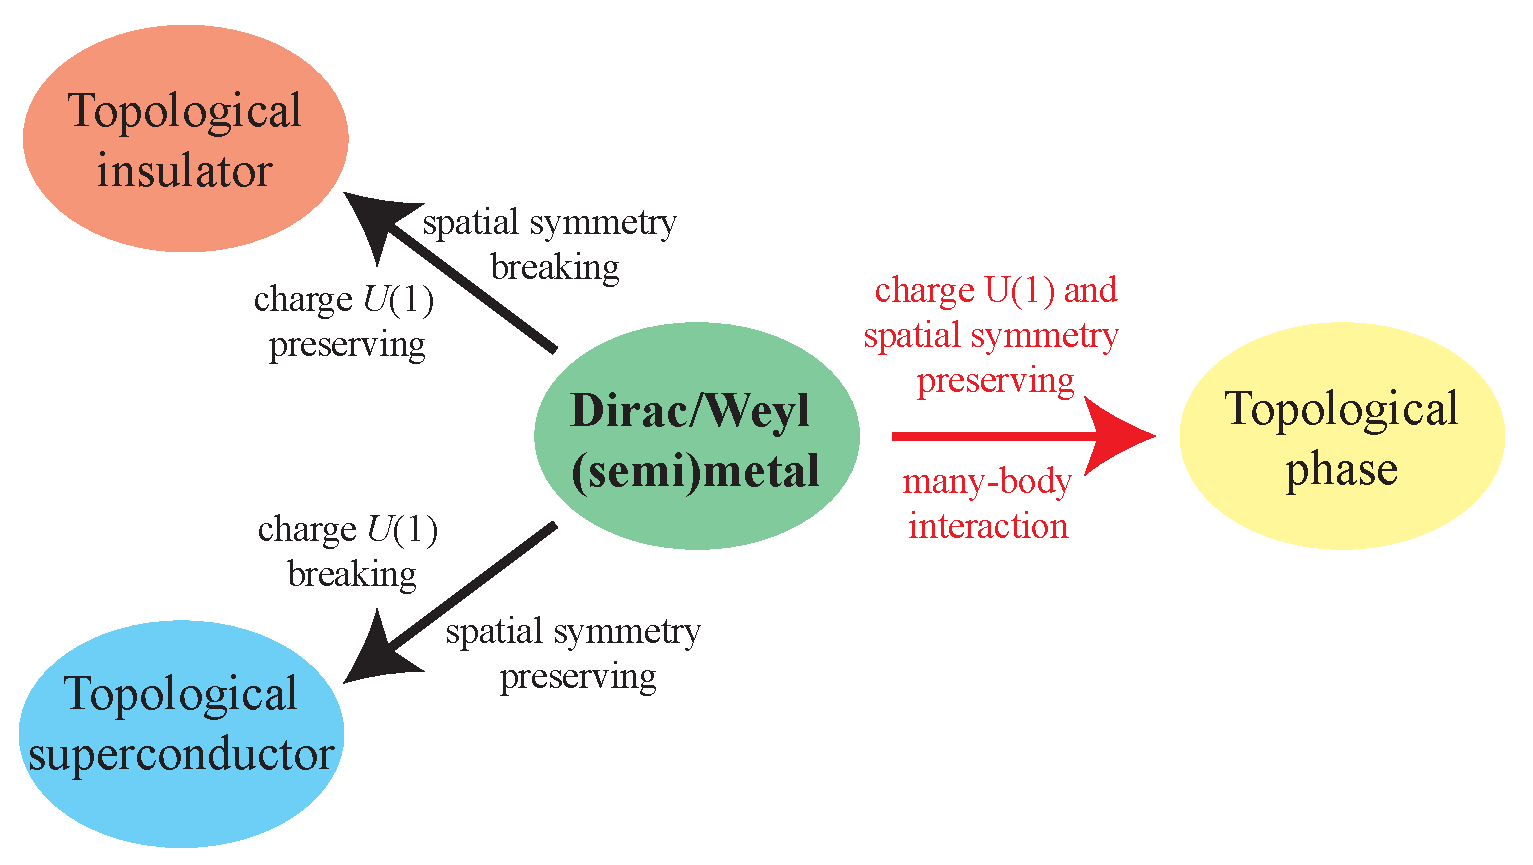
\includegraphics[width=0.9\textwidth]{intro}
	\caption{Symmetry breaking single-body gapping versus symmetry preserving many-body gapping of a Dirac/Weyl (semi)metal.}\label{fig:intro}
\end{figure}

Dirac/Weyl (semi)metals are the origins of a wide variety of topological phases in three dimensions (see Fig.~\ref{fig:intro}). By introducing a spatial or charge $U(1)$ symmetry-breaking single-body mass, they can be turned into a topological insulator or superconductor. The focus of this manuscript is on symmetry-preserving many-body gapping interactions. The resulting insulating topological phase can carry long-range entanglement and a non-trivial topological order. Similar phenomena were theoretically studied on the Dirac surface state of a topological insulator~\cite{WangPotterSenthilgapTI13,MetlitskiKaneFisher13b,ChenFidkowskiVishwanath14,BondersonNayakQi13} and the Majorana surface state of a topological superconductor~\cite{LukaszChenVishwanath,MetlitskiFidkowskiChenVishwanath14}, where symmetry-preserving many-body gapping interactions are possible and lead to non-trivial surface topological orders that support anyonic quasiparticle excitations.

Symmetry-preserving gapping interactions cannot be studied using a single-body mean-field theory. This is because the Dirac/Weyl (semi)metallic phase is protected by symmetries in the single-body setting and any mean-field model with an excitation energy gap must therefore break the symmetry either explicitly or spontaneously. The coupled wire construction can serve as a powerful tool in building an exactly-solvable interacting model and understanding many-body topological phases of this sort. The construction involves a highly anisotropic approximation where the electronic degrees of freedom are confined along an array of continuous one-dimensional wires. Inspired by sliding Luttinger liquids~\cite{OHernLubenskyToner99,EmeryFradkinKivelsonLubensky00,VishwanathCarpentier01,SondhiYang01,MukhopadhyayKaneLubensky01}, the coupled wire construction was pioneered by Kane, Mukhopadhyay and Lubensky~\cite{KaneMukhopadhyayLubensky02} in the study of Laughlin~\cite{Laughlin83} and Haldane-Halperin hierarchy~\cite{Haldane83,Halperin84} fractional quantum Hall states. Later, this theoretical technique was applied in more general fractional quantum Hall states~\cite{TeoKaneCouplewires,KlinovajaLoss14,MengStanoKlinovajaLoss14,SagiOregSternHalperin15,KaneSternHalperin17}, anyon models~\cite{OregSelaStern14,StoudenmireClarkeMongAlicea15}, spin liquids~\cite{MengNeupertGreiterThomale15,GorohovskyPereiraSela15}, (fractional) topological insulators~\cite{NeupertChamonMudryThomale14,KlinovajaTserkovnyak14,SagiOreg14,SagiOreg15,SantosHuangGefenGutman15} and superconductors~\cite{mongg2,SeroussiBergOreg14}, as well as the exploration of symmetries and dualities~\cite{MrossAliceaMotrunich16,MrossAliceaMotrunich17}. Moreover, coupled wire construction has already been used to investigate three dimensional fractional topological phases~\cite{Meng15,IadecolaNeupertChamonMudry16,IadecolaNeupertChamonMudry17} and Weyl (semi)metal~\cite{Vazifeh13} even in the strongly-correlated fractional setting~\cite{MengGrushinShtengelBardarson16}. 

The microscopic symmetry-preserving many-body interactions in the Dirac surface state on a topological insulator was discussed by Mross, Essin and Alicea in Ref.\cite{MrossEssinAlicea15}. They mimicked the surface Dirac modes using a coupled wire model and proposed explicit symmetric many-body interactions that lead to a variation of gapped and gapless surface states. Motivated by this and also using a coupled wire construction, the microscopic symmetry-preserving many-body gapping of the Majorana topological superconducting surface state was studied by one of us in Ref.\cite{SahooZhangTeo15}. 

In this article, we focus on (i) a coupled wire realization of a Dirac/Weyl (semi)metallic phase protected by antiferromagnetic time-reversal (\hypertarget{AFTR}{AFTR}) and screw twofold rotation symmetries, (ii) a set of exactly-solvable inter-wire many-body interactions that introduces a finite excitation energy gap while preserving the symmetries, and (iii) an interaction-enabled (semi)metallic electronic phase which is otherwise forbidden by symmetries in the single-body setting.

\section{Coupled Wire model of Dirac Semimetals}\label{sec:DiracSemimetal}
We begin with a Dirac semimetal in three dimensions. It consists of a pair of massless Weyl fermions with opposite chiralities. In this article we do not distinguish between a Dirac and a Weyl semimetal. This is because the fermion doubling theorem~\cite{Nielsen_Ninomiya_1981,NielsenNinomiyaPLB1981,NielsenNinomiya83} and the absence of the Adler-Bell-Jackiw anomaly~\cite{Adler69,BellJackiw69} require Weyl fermions to always come in pairs in a three dimensional lattice system. A Weyl semimetal therefore carries the same low energy degrees of freedom as a Dirac semimetal. We refer to the case when the pair of Weyl fermions are separated in momentum space as a translation symmetry protected Dirac semimetal. Here, we assume the simplest case where the two Weyl fermions overlap in energy-momentum space. Its low-energy band Hamiltonian takes the spin-orbit coupled form \begin{align}H^0_{\mathrm{Dirac}}({\bf k})=\hbar v{\bf k}\cdot\vec{s}\mu_z \,, \label{DiracHam0}\end{align} where $\vec{s}=(s_x,s_y,s_z)$ are the spin-$1/2$ Pauli matrices, and $\mu_z=\pm1$ indexes the two Weyl fermions.

\begin{figure}[htbp]
	\centering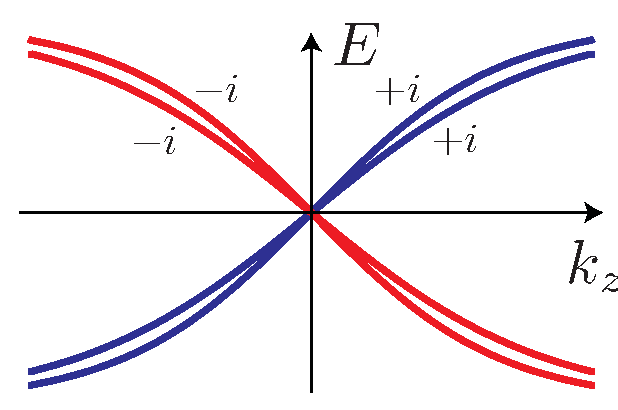
\includegraphics[width=0.5\textwidth]{Diracbands}
	\caption[The two pairs of counter-propagating Dirac bands.]{The two pairs of counter-propagating Dirac bands along the $k_z$-axis distinguished by eigenvalues of $C_2=\pm i$.}\label{fig:Diracbands}
\end{figure}

Normally the masslessness of the Dirac system is protected by a set of symmetries. Here, we assume the time reversal (TR) $\mathcal{T}$, which is represented in the single-body picture by the spinful operator $\hat{T}=is_y\mathcal{K}$ where $\mathcal{K}$ is the complex conjugation operator, and a twofold rotation $C_2$ about the $z$-axis. In the case when $\mu_z$ has a non-local origin such as sublattice or orbital, it can enter the rotation operator. We assume $\mathcal{C}_2$ is represented in the single-body picture by $\hat{C}_2=is_z\mu_z$. It squares to minus one in agreement with the fermionic statistics, and commutes with the local \TR operator. In momentum space, $\mathcal{T}$ flips ${\bf k}\to-{\bf k}$ while $C_2$ rotates $(k_x,k_y,k_z)\to(-k_x,-k_y,k_z)$. The band Hamiltonian \eqref{DiracHam0} shares simultaneous eigenstates with $C_2$ along the $k_z$-axis. The two forward moving bands have $C_2$ eigenvalues $+i$ while the two backward moving ones have $C_2$ eigenvalues $-i$ (see Fig.~\ref{fig:Diracbands}). Therefore the band crossing is $C_2$-protected while the fourfold degeneracy is pinned at ${\bf k}=0$ because of \TR symmetry. Noticing that each of the $C_2=\pm i$ sector along the $k_z$-axis is chiral (i.e.~consisting of a single propagating direction), it violates the fermion doubling theorem~\cite{Nielsen_Ninomiya_1981,NielsenNinomiyaPLB1981} and is anomalous. This can be resolved by assuming the $C_2$ symmetry is actually a non-symmorphic screw rotation in the microscopic lattice limit and squares to a primitive lattice translation in $z$. $k_z$ is now periodically defined (up to $2\pi/a$) and the two $C_2$ eigen-sectors wraps onto each other after each period. Focusing on the continuum limit where $k_z$ is small (when compared with $2\pi/a$), $C_2^2=-e^{ik_za}\approx-1$ and the $C_2$ symmetry behaves asymptotically as a proper rotation.

The primary focus of this article is to explore symmetry preserving/enabled interacting topological states that originate from the massless Dirac system. Contrary to its robustness in the single-body non-interacting picture, we show that the 3D Dirac fermion can acquire a many-body mass gap without violating the set of symmetries. To illustrate this, we first make use of the fact that the Dirac system can be turned massive by breaking symmetries. Symmetry breaking inter-valley scatterings introduce two coexisting mass terms \begin{align}H_{\mathrm{Dirac}}({\bf k},{\bf r})=H_{\mathrm{Dirac}}^0({\bf k})+m_x({\bf r})\mu_x+m_y({\bf r})\mu_y \,, \label{DiracHam}\end{align} where $m_x$ (or $m_y$) preserves (resp.~breaks) \TR, and both of them violate $C_2$. We allow slow spatial modulation of the mass parameters, which can be grouped into a single complex parameter $m({\bf r})=m_x({\bf r})+im_y({\bf r})$, and to be precise, momentum ${\bf k}$ should be taken as a differential operator $-i\nabla_{\bf r}$ when translation symmetry is broken. Non-trivial spatial windings of the symmetry breaking mass parameters give rise to topological line defects or vortices that host protected low-energy electronic degrees of freedom. Proliferation of interacting vortices then provides a theoretical path to multiple massive/massless topological phases while restoring and modifying the original symmetries as they emerge in the low-energy long-length scale effective theory.

\begin{figure}[htbp]
	\centering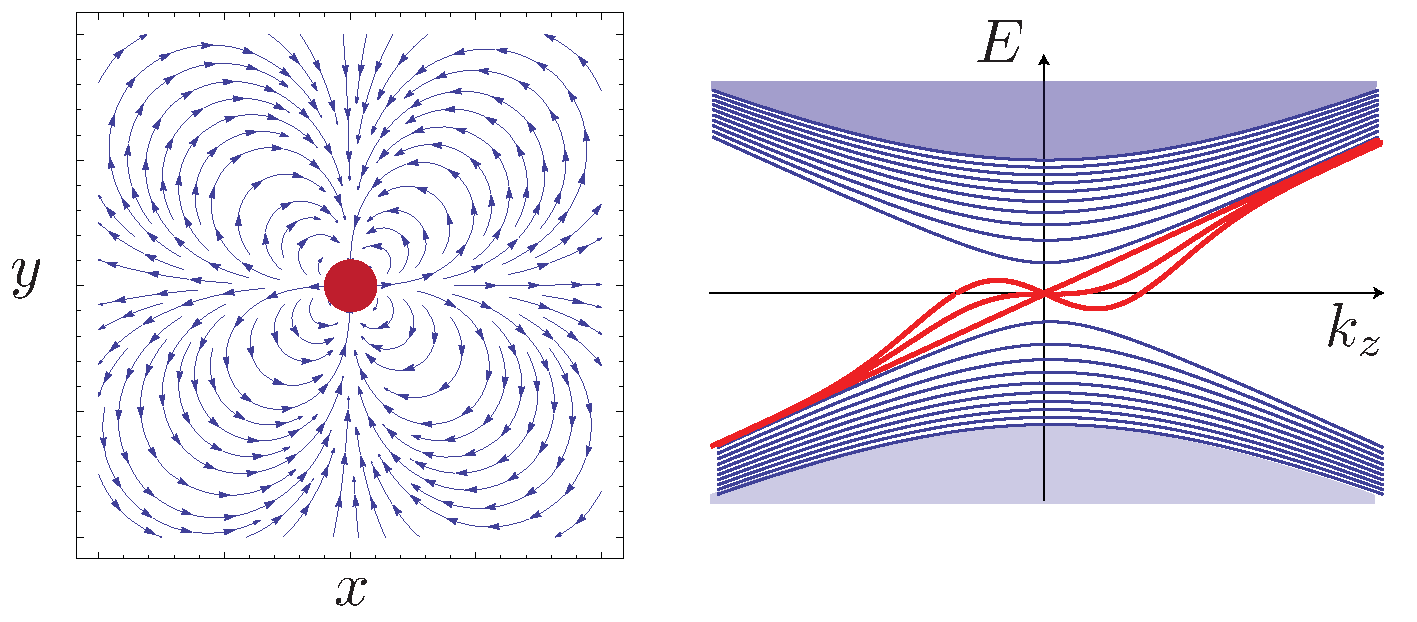
\includegraphics[width=0.8\textwidth]{Diracstring}
	\caption[Spatial winding of mass parameters around a Dirac string.]{Dirac string. (Left) Spatial winding of mass parameters around a Dirac string going out of the paper represented by the center red dot. Stream lines represent the vector field ${\bf m}({\bf r})=(m_x({\bf r}),m_y({\bf r}))$. (Right) Energy spectrum of chiral Dirac fermions. Blue bands represent bulk continuum. Red bands correspond to chiral Dirac fermions localized along the string.}\label{fig:Diracstring}
\end{figure}

A topological line defect is a vortex string of the mass parameter in three dimensions where the complex phase of $m({\bf r})=|m({\bf r})|e^{i\varphi({\bf r})}$ winds non-trivially around the string. The left diagram in Fig.~\ref{fig:Diracstring} shows the spatial modulation of $\varphi({\bf r})$ along the $xy$ cross-sectional plane normal to a topological line defect, which runs along the $z$ axis. In this example, the complex phase $\varphi({\bf r})$ winds by $6\pi$ around the line defect (represented by the red dot at the origin). The winding number of the complex phase in general can be evaluated by the line integral \begin{align}c=\frac{1}{2\pi}\oint_\mathcal{C}d\varphi({\bf r})=\frac{1}{2\pi i}\oint_\mathcal{C}\frac{\nabla_{\bf r}m({\bf r})}{m({\bf r})}\cdot d{\bf r} \,, \label{winding}\end{align} where $\mathcal{C}$ is a (righthanded) closed path that runs once around the (oriented) line defect. Eq.\eqref{winding} is always an integer given that the mass parameter $m({\bf r})$ is non-vanishing along $\mathcal{C}$.

Massless chiral Dirac fermions run along these topological line defects~\cite{TeoKane}. When focusing at $k_z=0$, the differential operator \eqref{DiracHam} with a vortex along the $z$-axis is identical to the 2D Jackiw-Rossi model~\cite{JackiwRossi81} with chiral symmetry $\gamma_5=s_z\mu_z$. Each zero energy mode corresponds to a massless chiral Dirac fermion with positive or negative group velocity in $z$ depending on the sign of its $\gamma_5$ eigenvalue. (For a concrete example, see appendix~\ref{sec:chiralmodesapp}) These quasi-one dimensional low-energy electronic modes are similar to those that run along the edge of 2D Landau levels and Chern insulators, except they are now embedded in three dimensions. Their wave functions extend along the defect string direction but are localized and exponentially decay away from the defect line. Moreover, such an electronic channel is chiral in the sense that there is only a single propagating direction. The energy spectrum of the topological line defect (for the example with winding number $c=3$) is shown in the right diagram of Fig.~\ref{fig:Diracstring}, in which, there are three chiral bands (red curves) inside the bulk energy gap representing the 3 chiral Dirac electrons. As a consequence of the chirality, the transport of charge and energy must also be uni-directional. The chiral electric and energy-thermal responses are respectively captured by the two conductances \begin{align}\sigma=\frac{\delta I_{\mathrm{electric}}}{\delta V}=\nu\frac{e^2}{h},\quad\kappa=\frac{\delta I_{\mathrm{energy}}}{\delta T}=c\frac{\pi^2k_B^2}{3h}T \,, \label{conductance}\end{align} where $\nu$ is the filling fraction if the chiral channel is supported by a 2D insulating bulk, and $c$ is called the chiral central charge. For the Dirac case, $c=\nu$ is the number of chiral Dirac channels. Here $c$ can be negative when the Dirac fermions oppose the preferred orientation of the topological line defect. In a more general situation, $c=c_R-c_L$ counts the difference between the number of forward propagating and backward propagating Dirac fermions. There is a mathematical index theorem~\cite{TeoKane,AtiyahSinger63,Nakaharabook} that identifies the topological winding number in \eqref{winding} and the analytic number of chiral Dirac fermions in \eqref{conductance}. Hence, there is no need to distinguish the two $c$'s. 

The massless chiral Dirac channels, described by the low-energy effective theory \begin{align}\mathcal{L}_{\mathrm{Dirac}}=i\sum_{a=1}^{c_R}\psi^\dagger_a(\partial_t+\tilde{v}\partial_x)\psi_a+i\sum_{b=c_R+1}^{c_R+c_L}\psi^\dagger_b(\partial_t-\tilde{v}\partial_x)\psi_b\label{lowenergy}\end{align} have an emergent conformal symmetry and the index $c=c_R-c_L$ is also the chiral central charge of the effective conformal field theory (\hypertarget{CFT}{CFT}). We refer to the primitive topological line defect with $c=\pm1$ that hosts one and only chiral Dirac fermion $\psi$ as a {\em Dirac string}. (It should not be confused with the Dirac magnetic flux string that connects monopoles.)

\begin{figure}[htbp]
	\centering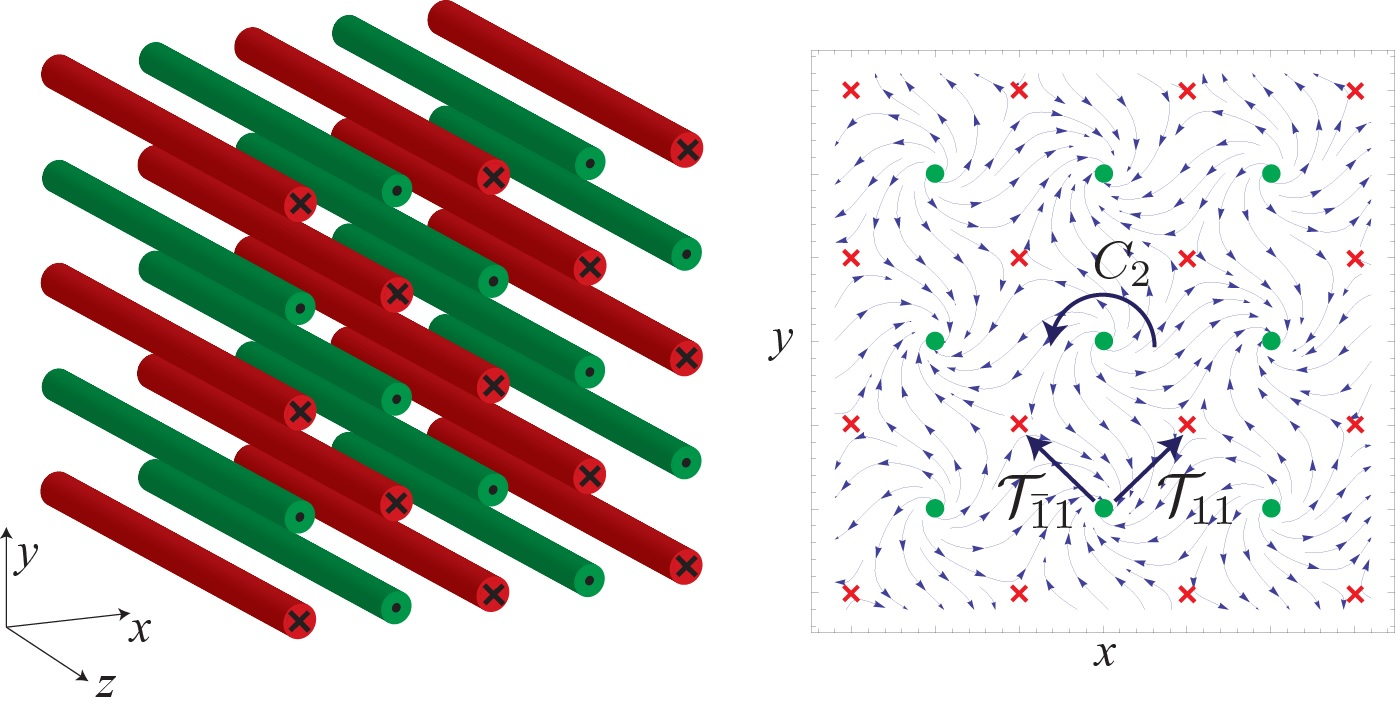
\includegraphics[width=0.9\textwidth]{vortexlattice.jpg}
	\caption[(Left) A 3D array of Dirac strings. (Right) Cross section of the array.]{(Left) A 3D array of Dirac strings. (Right) Cross section of the array. {\color{red}$\boldsymbol\times$} associates into-the-plane Dirac channel, {\color{green}$\bullet$} represents out-of-plane ones. Stream lines represent the configuration of the mass parameter vector field ${\bf m}({\bf r})=(m_x({\bf r}),m_y({\bf r}))$ of the vortex lattice.}\label{fig:vortexlattice}
	\centering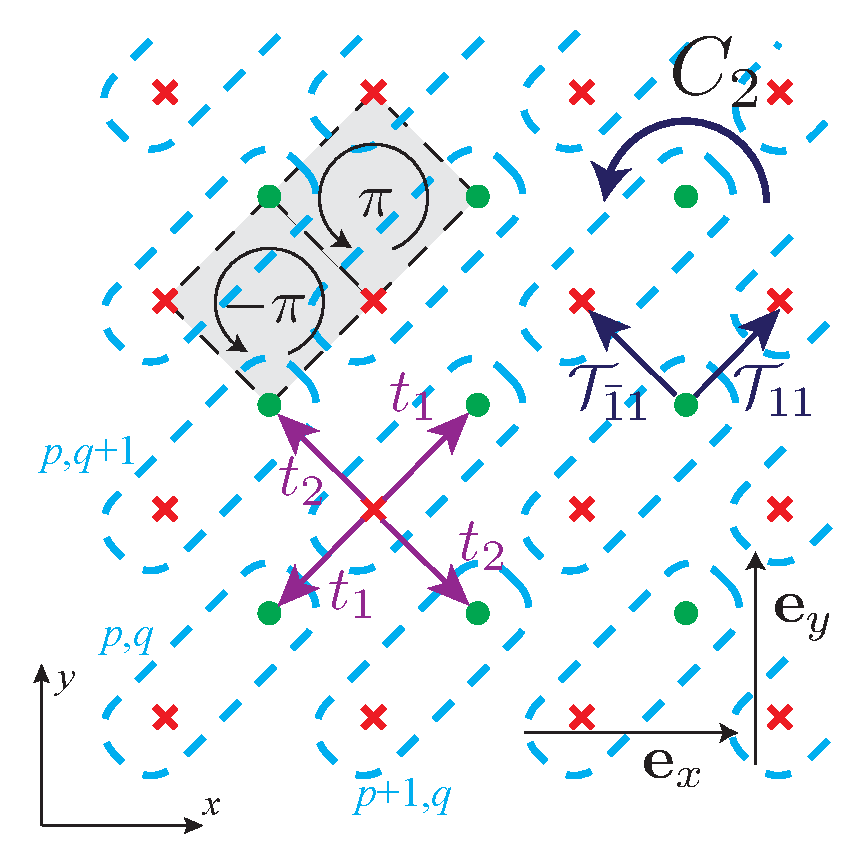
\includegraphics[width=0.5\textwidth]{WeylTB}
	\caption[Coupled Dirac wire model with tunneling amplitudes.]{Coupled Dirac wire model with tunneling amplitudes $t_1,t_2$. Each unit cell (dashed box) consists a pair of counter-propagating Dirac strings, {\color{red}$\boldsymbol\times$} and {\color{green}$\bullet$}. $\mathcal{T}_{11},\mathcal{T}_{\bar{1}1}$ are the two anti-ferromagnetic directions.}\label{fig:WeylTB}
\end{figure}

A three-dimensional array of Dirac strings (wires) can be realized as a vortex lattice of the mass parameter $m=m_x+im_y$ in a Dirac semimetal. For example, Fig.~\ref{fig:vortexlattice} shows a vortex lattice generated by the spatially-varying Dirac mass \begin{align}m({\bf r})=m_0\frac{\mathrm{sd}(x+iy)}{|\mathrm{sd}(x+iy)|},\label{Jacobielliptic}\end{align} where $\mathrm{sd}$ is the (rescaled) Jacobian elliptic function~\cite{ReinhardtWalker10} with simple zeros at $p+iq$ and poles at $(p+1/2)+i(q+1/2)$ for $p,q$ integers. It consists of vortices with alternating winding number $c=\pm1$ at the zeros and poles in a checkered board lattice configuration. On the cross section plot on the right side of Fig.~\ref{fig:vortexlattice}, there is a Dirac string with positive (or negative) winding at each {\color{green}$\bullet$} (resp. {\color{red}$\boldsymbol\times$}). Each vortex string has a chiral Dirac fermion running through it. Figure~\ref{fig:WeylTB} shows the same two-dimensional slice of the array, except suppressing the mass parameters which correspond to irrelevant microscopic high-energy degrees of freedom. We choose a unit cell labeled by $(p,q)$, its $x,y$ coordinates. Each has both a forward moving Dirac fermion $\psi_{p,q}^\odot$ (shown as {\color{green}$\bullet$}) and a backward moving one $\psi_{p,q}^\otimes$ (shown as {\color{red}$\boldsymbol\times$}). 

This array configuration breaks \TR as the symmetry would have reversed the chirality (i.e.~propagating direction) of each Dirac fermion. Instead, it has an emergent {\em anti-ferromagnetic time reversal} (AFTR) symmetry, which is generated by the operators $\mathcal{T}_{11}$ and $\mathcal{T}_{\bar{1}1}$ in the diagonal and off-diagonal directions. Each is composed of a time reversal operation and a half-translation by $({\bf e}_x+{\bf e}_y)/2$ or $(-{\bf e}_x+{\bf e}_y)/2$. \begin{gather}\mathcal{T}_{11}\psi_{p,q}^\otimes\mathcal{T}_{11}^{-1}=\psi_{p,q}^\odot,\quad\mathcal{T}_{11}\psi_{p,q}^\odot\mathcal{T}_{11}^{-1}=-\psi_{p+1,q+1}^\otimes\nonumber\\\mathcal{T}_{\bar{1}1}\psi_{p,q}^\otimes\mathcal{T}_{\bar{1}1}^{-1}=\psi_{p-1,q}^\odot,\quad\mathcal{T}_{\bar{1}1}\psi_{p,q}^\odot\mathcal{T}_{\bar{1}1}^{-1}=-\psi_{p,q+1}^\otimes \,. \label{AFTR}\end{gather} These \AFTR operators are non-local as they come with lattice translation parts. They are anti-unitary in the sense that $\mathcal{T}\alpha\psi\mathcal{T}^{-1}=\alpha^\ast\mathcal{T}\psi\mathcal{T}^{-1}$ and $\langle\mathcal{T}u|\mathcal{T}v\rangle=\langle u|v\rangle^\ast$ because the local time reversal symmetry is anti-unitary. %Normally the local \TR operation for a spinful fermion squares to minus one. However, the non-local nature of the \AFTR symmetry allows us to absorb the sign by a non-local gauge transformation (for example $\psi^{\otimes/\odot}_{p,q}\to(-1)^q\psi^{\otimes/\odot}_{p,q}$) so that no signs appear in \eqref{AFTR}. 
Similar to a spatial non-symmorphic symmetry, the \AFTR symmetries square to the primitive translation operators \begin{align}\mathcal{T}_{11}\mathcal{T}_{\bar{1}1}&=(-1)^F\mbox{translation}({\bf e}_y),\nonumber\\\mathcal{T}_{11}\mathcal{T}_{\bar{1}1}^{-1}&=\mbox{translation}({\bf e}_x),\label{AFTRalg}\end{align} where $(-1)^F$ is the fermion parity operator. Moreover they mutually commute $[\mathcal{T}_{11},\mathcal{T}_{\bar{1}1}]=0$. We notice in passing that the \AFTR symmetry is only an emergent symmetry in the low-energy effective theory. It is not preserved in the microscopic Dirac model \eqref{DiracHam} and is broken by the mass parameter, $m({\bf r})\neq m({\bf r}+({\bf e}_x\pm{\bf e}_y)/2)^\ast$. For instance, the Jacobian elliptic Dirac mass function \eqref{Jacobielliptic} actually has a periodic unit cell twice the size of that of the effective wire model in Fig.~\ref{fig:WeylTB}. On the other hand, the Dirac mass \eqref{Jacobielliptic} is odd under $C_2$, $m(C_2{\bf r})=-m({\bf r})$. This sign is canceled by the $C_2$ rotations of the Dirac matrices, $\hat{C}_2\mu_{x,y}\hat{C}_2^{-1}=-\mu_{x,y}$, that couple with the Dirac mass in the Hamiltonian \eqref{DiracHam}. Therefore the Dirac wire model in Fig.~\ref{fig:WeylTB} has a twofold axis along one of the Dirac string, say $\psi^\odot_{0,0}$. The Dirac channel fermions transform unitarily according to \begin{align}\mathcal{C}_2\psi^\odot_{p,q}\mathcal{C}_2^{-1}=i\psi^\odot_{-p,-q},\quad\mathcal{C}_2\psi^\otimes_{p,q}\mathcal{C}_2^{-1}=-i\psi^\otimes_{-p+1,-q+1},\label{C2}\end{align} where the factor of $i$ ensures the fermionic $-1$ twist phase for a $2\pi$ rotation, and the second eqaulity in \eqref{C2} is determined by the first one together with \eqref{AFTR} and the symmetry relations \begin{gather}\mathcal{C}_2\mathcal{T}_{11}=(-1)^F\mathcal{T}_{11}^{-1}\mathcal{C}_2,\quad\mathcal{C}_2\mathcal{T}_{\bar{1}1}=(-1)^F\mathcal{T}_{\bar{1}1}^{-1}\mathcal{C}_2.\label{C2Trelation}\end{gather} Again, in order for the rotation symmetric wire model to be free of anomalies, $C_2$ should really be a screw rotation with respect to some microscopic lattice that has become irrelevant in the low-energy continuum picture. \begin{align}\mathcal{C}_2^2=(-1)^F\mathrm{translation}(a{\bf e}_z)\approx(-1)^F.\label{C2square}\end{align}

When adjacent vortex strings are near each other, their Dirac fermion wave functions overlap and there are finite amplitudes of electron tunneling. We construct a coupled Dirac wire model of nearest-wire single-body backscattering processes with $\pm\pi$ fluxes across each diamond square (Fig.~\ref{fig:WeylTB}), where the tunneling amplitude $t_1$ (or $t_2$) in the $(11)$ (resp.$(\bar{1}1)$) direction is imaginary (resp.~real). \begin{align}\mathcal{H}=&\sum_{p,q}\hbar\tilde{v}\left({\psi_{p,q}^\odot}^\dagger k_z\psi_{p,q}^\odot-{\psi_{p,q}^\otimes}^\dagger k_z\psi_{p,q}^\otimes\right)\nonumber\\&+it_1\left({\psi_{p,q}^\odot}^\dagger\psi_{p,q}^\otimes-{\psi_{p-1,q-1}^\odot}^\dagger\psi_{p,q}^\otimes\right)+h.c.\label{WeylTBHam}\\&+t_2\left({\psi_{p-1,q}^\odot}^\dagger\psi_{p,q}^\otimes-{\psi_{p,q-1}^\odot}^\dagger\psi_{p,q}^\otimes\right)+h.c.\nonumber \,, \end{align} where the first line is the kinetic Hamiltonian of individual Dirac channels under the Fourier transformation $-i\partial_z\leftrightarrow k_z$ along the wire direction. This tight-binding Hamiltonian preserves the \AFTR symmetry \eqref{AFTR}, $\mathcal{T}\mathcal{H}\mathcal{T}^{-1}=\mathcal{H}$. Fourier transformation of the square lattice $\vec\psi_{p,q}=\int\frac{dk_xdk_y}{(2\pi)^2}e^{-i(k_xp+k_yq)}\vec\psi_{\bf k}$, $\vec\psi=(\psi^\odot,\psi^\otimes)$ turns \eqref{WeylTBHam} into $\mathcal{H}=\int\frac{dk_xdk_y}{(2\pi)^2}\vec\psi_{\bf k}^\dagger H(k)\vec\psi_{\bf k}$, where \begin{align}H({\bf k})=\left(\begin{array}{*{20}c}\hbar\tilde{v}k_z&g(k_x,k_y)\\g^\ast(k_x,k_y)&-\hbar\tilde{v}k_z\end{array}\right)\label{BlochHam}\end{align} is the Bloch band Hamiltonian, for $g(k_x,k_y)=it_1(1-e^{-i(k_y+k_x)})+t_2(e^{-ik_x}-e^{-ik_y})$. Here momentum ${\bf k}$ lives in the ``liquid crystal" Brillouin zone (\hypertarget{BZ}{BZ}) where $-\pi\leq k_x,k_y\leq\pi$ and $-\infty<k_z<\infty$ (in the continuum limit $a\to0$ and $\pi/a\to\infty$). 

\begin{figure}[htbp]
	\centering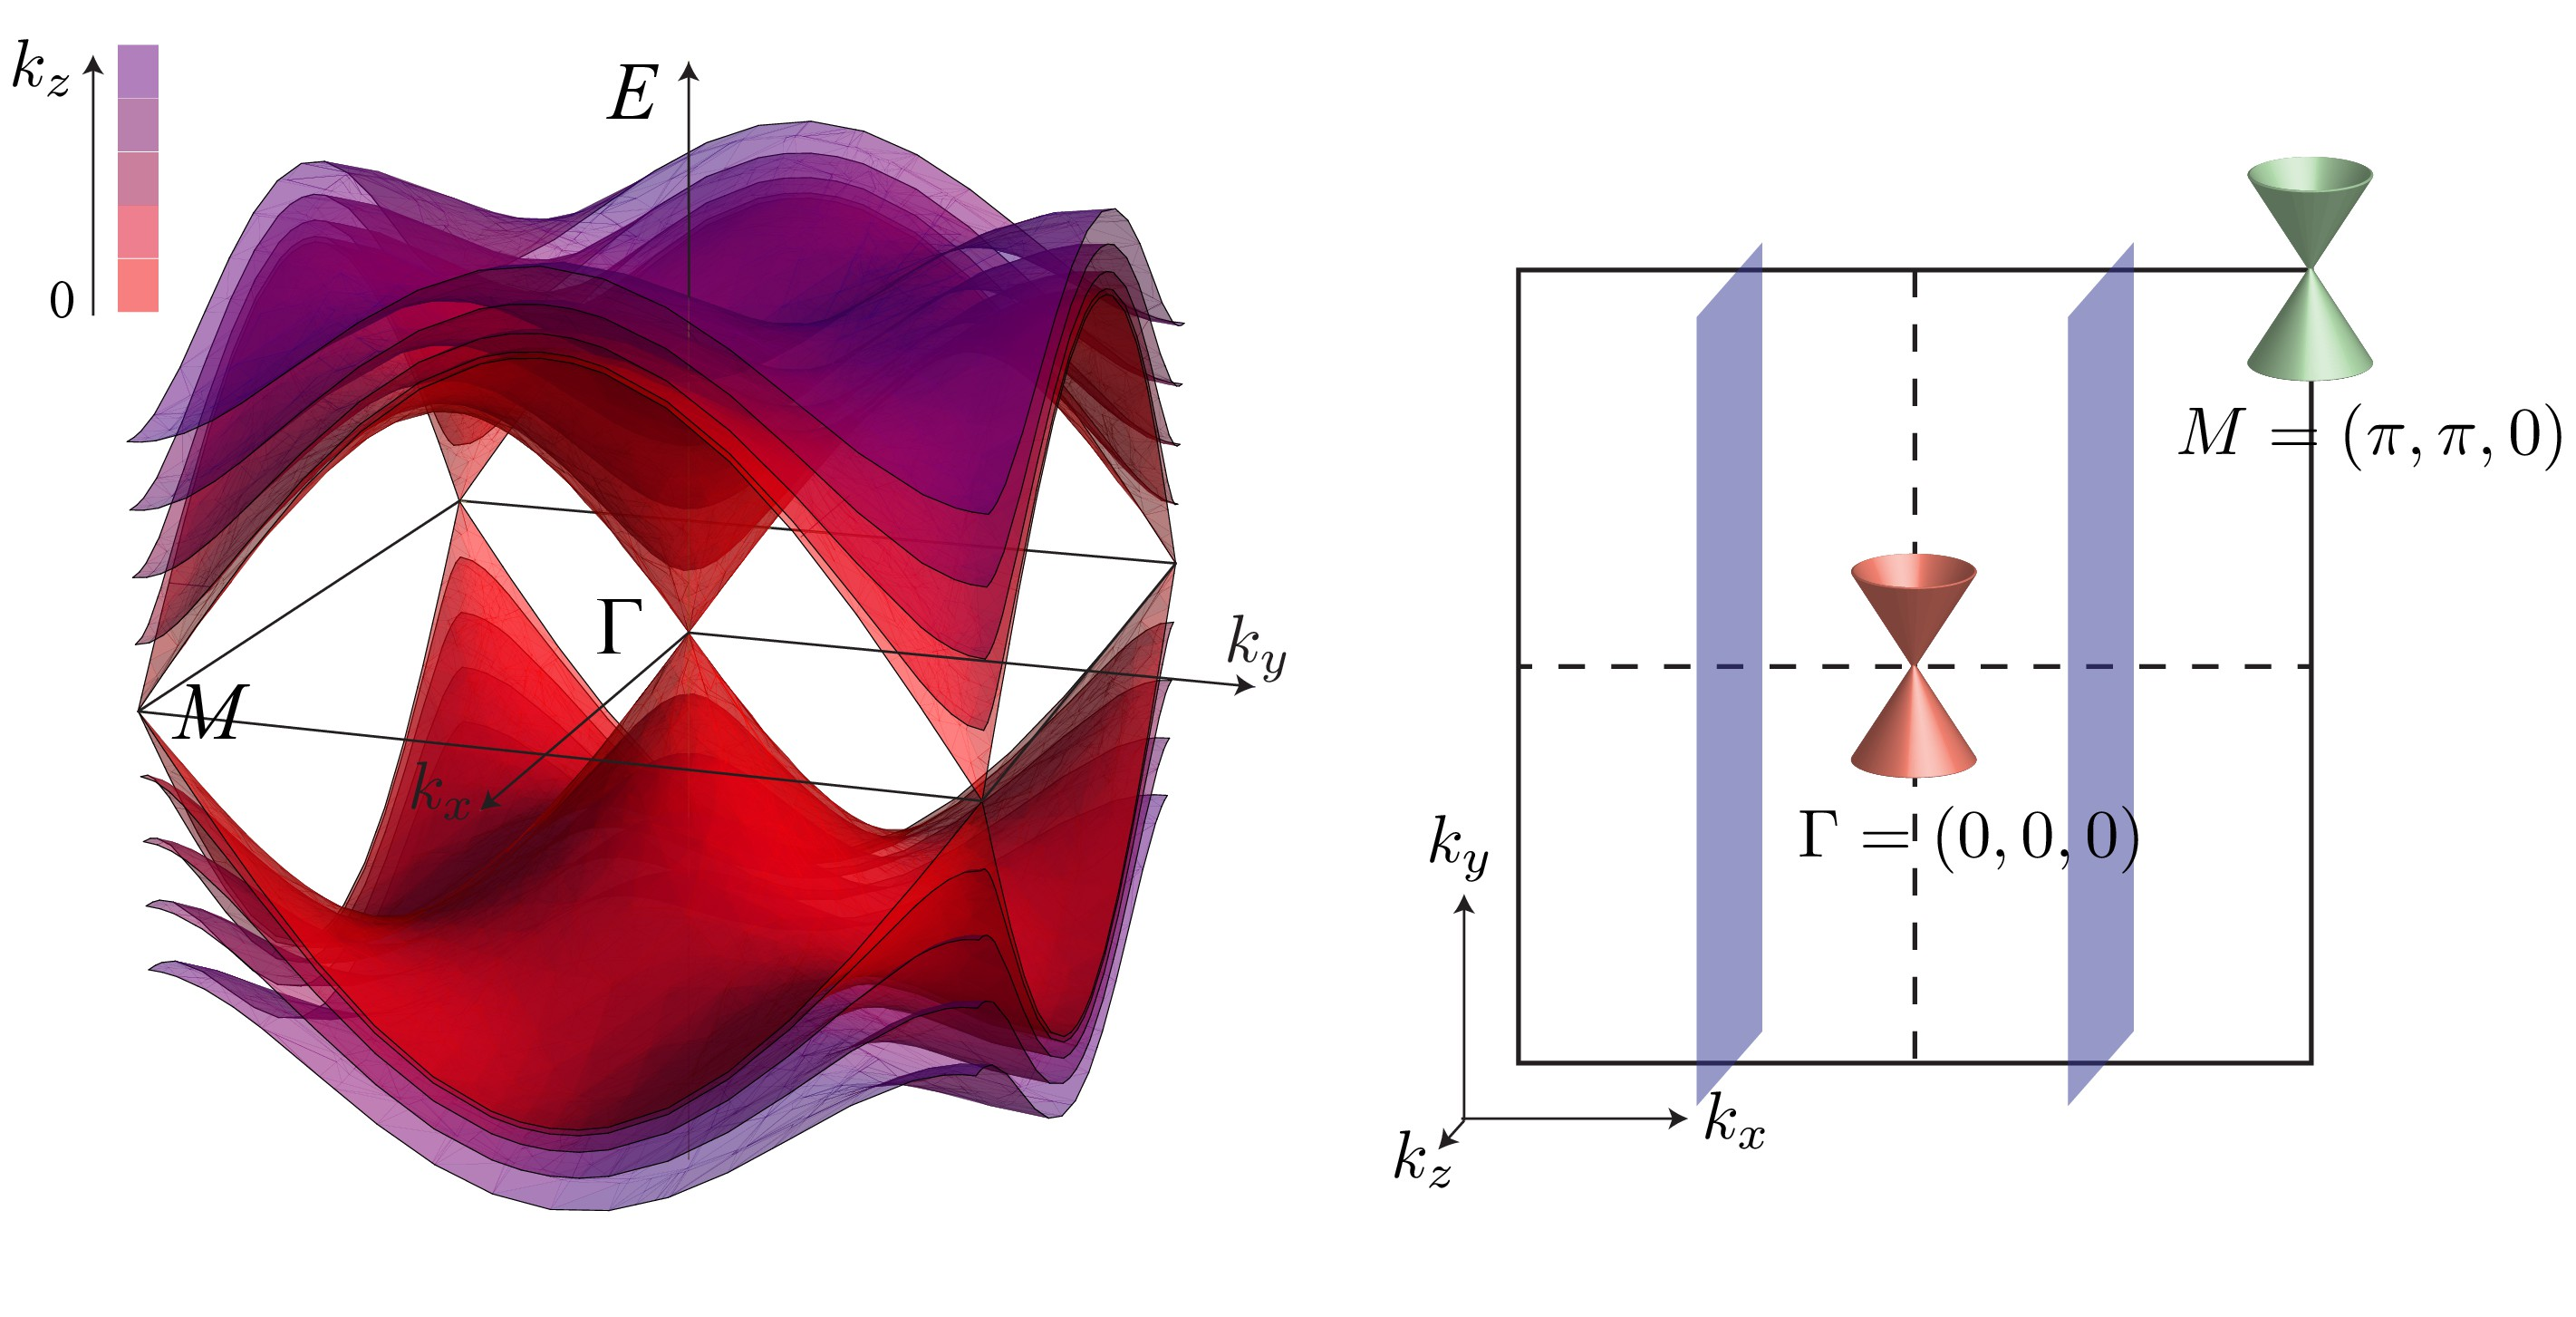
\includegraphics[width=0.9\textwidth]{Weylspectrumjpg.jpg}
	\caption{Energy spectrum of the coupled Dirac wire model \eqref{WeylTBHam}.}\label{fig:Weylspectrum}
\end{figure}

The energy spectrum of the two-band model is given by $E_\pm({\bf k})=\pm\sqrt{|g(k_x,k_y)|^2+\hbar^2\tilde{v}^2k_z^2}$ (see Fig.~\ref{fig:Weylspectrum}).
It gives two linearly dispersing Weyl cones of opposite chiralities in the \BZ centered at $K^+_0=\Gamma=(0,0,0)$ and $K^-_0=M=(\pi,\pi,0)$. Near these points, the Hamiltonians are of the linear form $H(K_0^\pm+\delta{\bf k})=\hbar\delta{\bf k}^TV^\pm\vec\sigma+O(\delta k^2)$, where $\vec\sigma=(\sigma_x,\sigma_y,\sigma_z)$ are Pauli matrices acting on the $(\psi^\odot,\psi^\otimes)$ degrees of freedom. The velocity matrices are \begin{align}\hbar V^\pm=\left(\begin{array}{ccc}-t_1&\pm t_2&0\\-t_1&\mp t_2&0\\0&0&\hbar\tilde{v}\end{array}\right),\end{align} whose determinant's %$\det(\hbar V)=\pm2\hbar\tilde{v}t_1t_2$ 
sign decides the $\pm$ chirality of the Weyl fermion at $\Gamma$ and $M$, i.e.~the $\pm1$ Fermi surface Chern invariants~\cite{WanVishwanathSavrasovPRB11,Ashvin_Weyl_review,RMP}. %Expanding about the two Weyl points and ignoring higher order terms gives $H(X^{\pm} + \delta {\mathbf{k}})= -t_1 (\delta k_x + \delta k_y) \sigma_x  \mp t_2 (\delta k_x - \delta k_y) \sigma_y  + v \delta k_z \sigma_z$.
The \AFTR symmetries \eqref{AFTR} in the single-body picture are expressed under Fourier transformation as \begin{gather}\mathcal{T}_{11}\vec\psi_{\bf k}\mathcal{T}_{11}^{-1}=T_{11}({\bf k})\vec\psi_{-\bf k},\quad\mathcal{T}_{\bar{1}1}\vec\psi_{\bf k}\mathcal{T}_{\bar{1}1}^{-1}=T_{\bar{1}1}({\bf k})\vec\psi_{-\bf k},\nonumber\\T_{11}({\bf k})=\left(\begin{array}{ccc}0&-e^{i(k_x+k_y)}\\1&0\end{array}\right)\mathcal{K},\nonumber\\T_{\bar{1}1}({\bf k})=\left(\begin{array}{ccc}0&-e^{ik_y}\\e^{-ik_x}&0\end{array}\right)\mathcal{K},\label{AFTRk}\end{gather} where $\mathcal{K}$ is the complex conjugation operator. They satisfy the appropriate algebraic relations \eqref{AFTRalg} in momentum space \begin{gather}T_{11}(-{\bf k})T_{\bar{1}1}({\bf k})=T_{\bar{1}1}(-{\bf k})T_{11}({\bf k})=-e^{-ik_y}\nonumber\\T_{11}(-{\bf k})T_{\bar{1}1}({\bf k})^{-1}=T_{\bar{1}1}(-{\bf k})^{-1}T_{11}({\bf k})=e^{-ik_x}\end{gather} and the coupled wire model \eqref{BlochHam} is \AFTR symmetric \begin{align}T_{11}({\bf k})H({\bf k})&=H(-{\bf k})T_{11}({\bf k}),\nonumber\\T_{\bar{1}1}({\bf k})H({\bf k})&=H(-{\bf k})T_{\bar{1}1}({\bf k}).\label{WeylTBT11}\end{align} The Weyl points are at time reversal invariant momenta (\hypertarget{TRIM}{TRIM}) $K^\pm_0\equiv-K^\pm_0$ (modulo the reciprocal lattice $2\pi\mathbb{Z}^2$), and the \AFTR operators $T_{11}(K^\pm_0)=-i\sigma_y\mathcal{K}$ and $T_{\bar{1}1}(K^\pm_0)=\mp i\sigma_y\mathcal{K}$ square to minus one. Hence the Weyl points are not only protected by the non-vanishing Fermi surface Chern invariant but also the Kramers' theorem. In addition, the model is also $C_2$ symmetric \begin{align}C_2({\bf k})H({\bf k})=H(C_2{\bf k})C_2({\bf k}) \,, \label{WeylTBC2}\end{align} where the twofold symmetry \eqref{C2} is represented in the single-body picture by a diagonal matrix \begin{align}\mathcal{C}_2\vec\psi_{\bf k}\mathcal{C}_2^{-1}=C_2({\bf k})\vec\psi_{C_2\bf k},\quad C_2({\bf k})=\left(\begin{array}{*{20}c}i&0\\0&-ie^{-i(k_x+k_y)}\end{array}\right)\label{C2k}\end{align} (suppressing the screw phase $e^{-ik_za/2}$ in the continuum limit $a\to0$). It agrees with the fermion statistics \eqref{C2square} $C_2(-k_x,-k_y,k_z)C_2(k_x,k_y,k_z)=-1$, and the algebraic relations \eqref{C2Trelation} with the \AFTR operators \begin{align}C_2(-{\bf k})T_{11}({\bf k})&=-T_{11}(C_2{\bf k})^{-1}C_2({\bf k})\nonumber\\C_2(-{\bf k})T_{\bar{1}1}({\bf k})&=-T_{\bar{1}1}(C_2{\bf k})^{-1}C_2({\bf k})\end{align} for $C_2{\bf k}=(-k_x,-k_y,k_z)$.

\subsection{The anomalous Dirac semimetal}\label{sec:anomaly}
We notice that the coupled wire Dirac model \eqref{WeylTBHam} and its massless energy spectrum in Fig.~\ref{fig:Weylspectrum} are anomalous with respect to the \AFTR symmetries $\mathcal{T}_{11}$ and $\mathcal{T}_{\bar{1}1}$ as well as the $C_2$ symmetry if it is proper symmorphic and not a screw rotation. This means that it cannot be realized in a single-body three dimensional lattice system with the \AFTR or $C_2$ symmetries. In a sense, it is not surprising at all since the chiral Dirac strings that constitute \eqref{WeylTBHam} are themselves violating fermion doubling~\cite{Nielsen_Ninomiya_1981,NielsenNinomiyaPLB1981}. Here we further elaborate on the anomalous Dirac spectrum (Fig.~\ref{fig:Weylspectrum}) where the pair of Weyl points are separately located at two \TRIM $K^\pm_0$. We also comment on the non-trivial consequence of the anomaly and pave the path for later discussion on many-body interactions.

We begin with two 2D planes in momentum space parallel to $k_yk_z$ located at $k_x=\pm\pi/2$. They are represented by the two blue planes in Fig.~\ref{fig:Weylspectrum}. The \AFTR or $C_2$ symmetries require the Chern invariants \begin{align}\mathrm{Ch}_1=\frac{i}{2\pi}\int\mathrm{Tr}(P\partial_{k_y}P\partial_{k_z}P)dk_ydk_z\label{1stChern}\end{align} at $k_x=\pm\pi/2$ to be opposite, where $P({\bf k})=(1-H({\bf k})/|E({\bf k})|)/2$ is the projection operator onto the negative energy band. This is because the \AFTR symmetry is anti-unitary and preserves the orientation of the $k_yk_z$ plane, whereas $C_2$ is unitary but reverses the orientation of the $k_yk_z$ plane. (See appendix~\ref{sec:Chernapp} for a detailed proof.) On the other hand, the two Chern invariants along the two planes must differ by 1 because they sandwich a single Weyl point at $\Gamma$. This forces the Chern invariants to be a half integer $\mathrm{Ch}_1=\pm1/2$, which is anomalous.

While the $C_2$ anomaly can be resolved simply by doubling the unit cell and assuming it originates from a microscopic non-symmorphic screw axis, the \AFTR anomaly is stronger because the two antiferromagnetic combinations \eqref{AFTRalg} generate lattice translations and fix the unit cell size. There are three resolutions. \begin{enumerate}\item The \AFTR symmetries are broken by high energy degrees of freedom when $k_z$ is large. \item The spectrum in Fig.~\ref{fig:Weylspectrum} is the holographic 3D boundary spectrum of an \AFTR symmetric weak topological insulator in 4D. \item The spectrum is generated by strong many-body interaction non-holographically in 3D.\end{enumerate} Below we discuss the first two resolutions, and we leave the many-body interaction-enabled situation to Sec.~\ref{sec:intenable}.

\subsubsection{Broken symmetries and coarse-graining}\label{sec:brokensymmetry}
The mapping between the original Dirac fermion model and the emergent Dirac fermion model from a coupled-wire construction can be qualitatively understood as a coarse-graining procedure. Here, the high-energy microscopic electronic degrees of freedom are integrated out. The procedure can be repeated indefinitely and resembles a real-space renormalization. For example, the gapless Dirac electronic structure of the coupled wire model can acquire a finite mass by symmetry-breaking dimerizations. These dimerizations can be arranged in a topological manner that spatially wind non-trivially around a collective vortex. These second-stage vortices can subsequently be assembled into an array similar to the previous construction except now with a longer lattice constant. The system again recovers a massless Dirac spectrum under inter-vortex electron tunneling in low-energy and long length scale. The mapping therefore establishes an equivalence between the continuous isotropic massless Dirac fermion and the semi-discrete anisotropic coupled Dirac wire model.

In the present case when the chiral Dirac channels originate from vortex strings in an underlying microscopic Dirac insulator, the spatial modulation of mass parameters $m({\bf r})$ actually violate one of the \AFTR symmetries, $m({\bf r})^\ast\neq m({\bf r}+({\bf e}_x\pm{\bf e}_y)/2)$, where $\ast$ stands for complex conjugation. For instance, since all elliptic functions must contain at least two zeros and two poles in its periodic cell, the Jacobian elliptic mass function \eqref{Jacobielliptic} has longer periods than ${\bf e}_x$ and ${\bf e}_y$ in Fig.~\ref{fig:WeylTB}, and thus must break $\mathcal{T}_{11}$ or $\mathcal{T}_{\bar{1}1}$. The symmetry is broken only in the ultra-violet limit at large $k_z$ where the chiral Dirac line nodes meet the microscopic bulk band (see Fig.~\ref{fig:Diracstring}) at high energy $\sim|m({\bf r})|$. In fact, the above anomalous argument shows that {\em all} mass parameter configurations that produce the 3D vortex lattice array (Fig.~\ref{fig:vortexlattice}) must either (a) break both the \AFTR symmetries $\mathcal{T}_{11}$ and $\mathcal{T}_{\bar{1}1}$, or (b) preserve one but violate translation so that the unit cell is enlarged and the two Weyl points collapse onto each other in momentum space. (See Figs.~\ref{fig:Chernstack} and \ref{fig:DiracTB}.)

For instance, the microscopic system can be connected to a stack of Chern insulating ribbons (or lowest Landau levels) with alternating chiralities shown in Fig.~\ref{fig:Chernstack}. Instead of being supported by vortices of Dirac mass, the chiral Dirac wires are now realized as edge modes of Chern insulating strips. Each 2D ribbon (represented by thick dashed dark blue lines) is elongated in the out-of-paper $z$-direction but is finite along the $(110)$ direction and holds counter-propagating boundary chiral Dirac channels. The dark blue arrows represent the orientations of the Chern ribbons that accommodate the boundary Dirac channels with the appropriate propagating directions. Here the Chern ribbon pattern in Fig.~\ref{fig:Chernstack}(a) breaks both \AFTR axes. The pattern in Fig.~\ref{fig:Chernstack}(b) preserves $\mathcal{T}_{\bar{1}1}$. However, translation symmetry is also broken and the coupled Dirac wire model now has an enlarged unit cell (light blue dashed boxes) that consists of two pairs of counter-propagating chiral Dirac channels. All Chern ribbon patterns must break the $C_2$ symmetry about a Dirac wire because each wire is connected to one and only one Chern ribbon in a particular direction.

\begin{figure}[htbp]
	\centering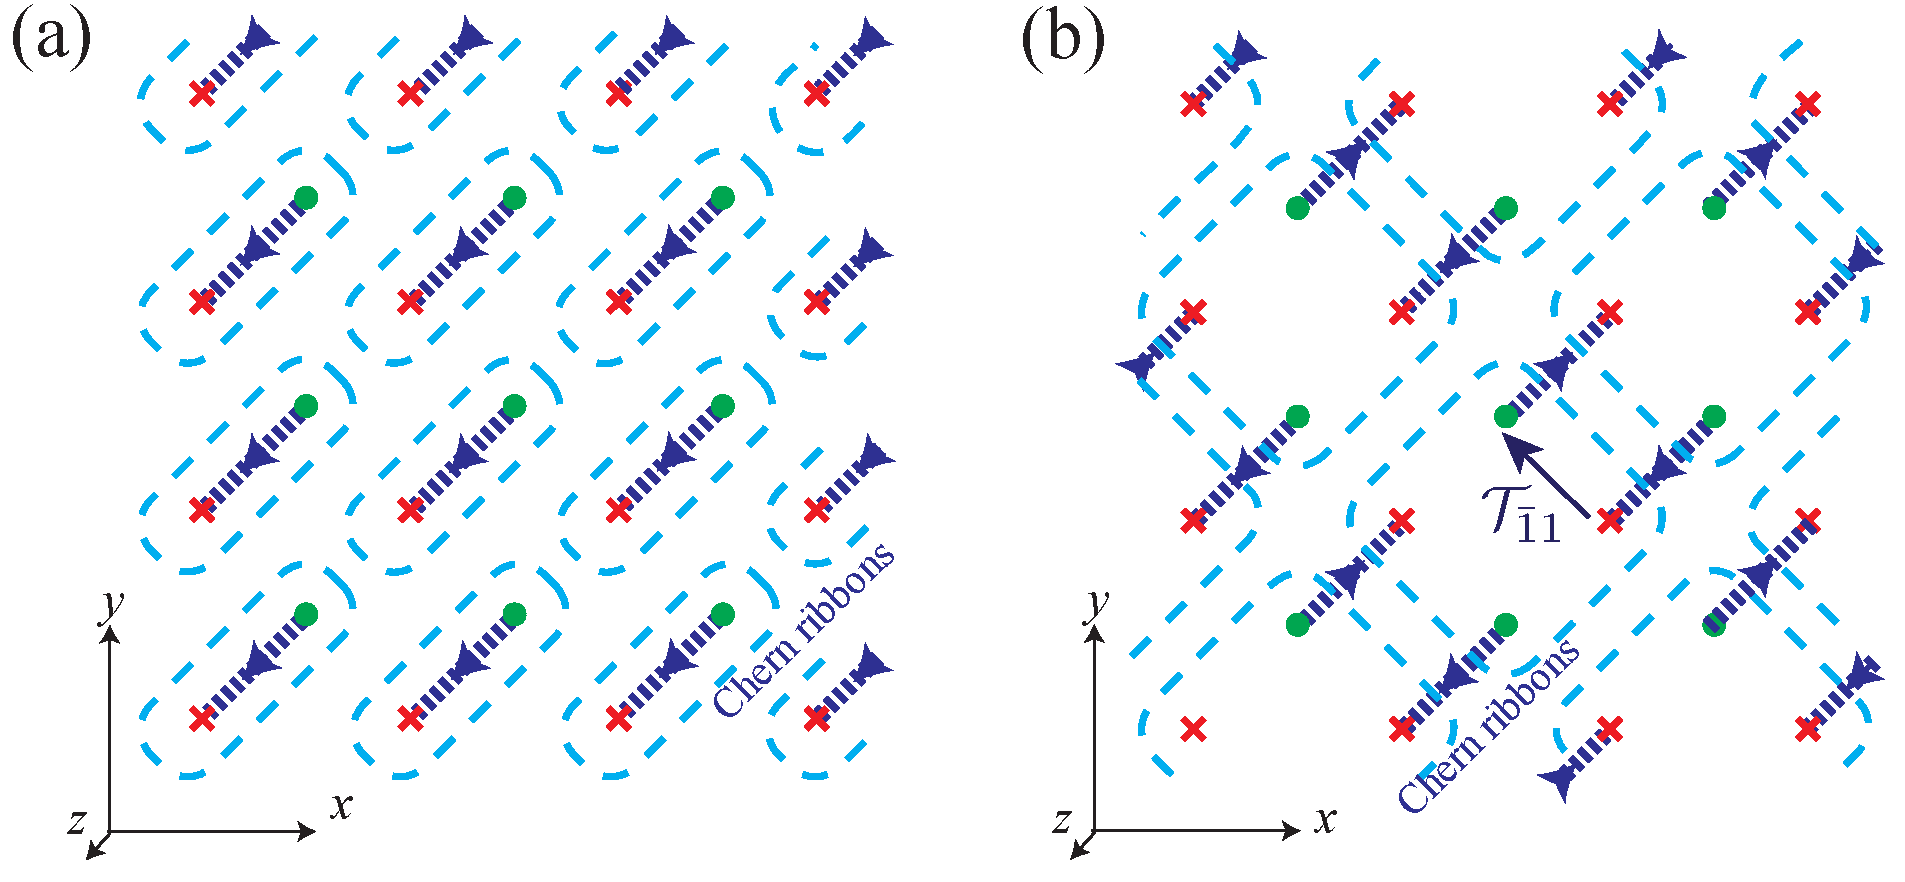
\includegraphics[width=0.9\textwidth]{Chernstack}
	\caption[Chiral Dirac channels realized on the edge of Chern insulating ribbons.]{Chiral Dirac channels ({\color{red}$\boldsymbol\times$} and {\color{green}$\bullet$}) realized on the edge of Chern insulating ribbons (dark blue directed lines) stacked along the $(\bar{1}10)$ normal direction.}\label{fig:Chernstack}
\end{figure}

Now we go back to the vortex lattice generated by the Jacobian elliptic Dirac mass function $m({\bf r})$ in \eqref{Jacobielliptic} and consider its symmetries. For this purpose, we use the symmetry properties of the (rescaled) Jacobian elliptic function~\cite{ReinhardtWalker10} \begin{align}&\mathrm{sd}(x+iy)=-\mathrm{sd}(x+1+iy)=-\mathrm{sd}(x+iy+i)\nonumber \,, \\&\mathrm{sd}\left(x+iy+\frac{1+i}{2}\right)=-i\frac{C}{\mathrm{sd}(x+iy)}\label{sdprop} \,, \\&\mathrm{sd}(-x-iy)=-\mathrm{sd}(x+iy)\nonumber \,,\end{align} where $C$ is some unimportant real constant that depends on the modulus of $\mathrm{sd}$ and will never appear in the mass function $m({\bf r})=m_0\mathrm{sd}(x+iy)/|\mathrm{sd}(x+iy)|$. We see from the minus sign in the first equation that the Jacobian elliptic function, and consequently the mass function, have primitive periods ${\bf e}_x\pm{\bf e}_y$ and therefore have a unit cell of size 2 (see Fig.~\ref{fig:DiracTB}(a)). Choosing $m_0=|m_0|e^{i\pi/4}$, we see from the second equation that $\mathcal{T}_{11}$ (or $\mathcal{T}_{\bar{1}1}$) is preserved (resp.~broken) \begin{align}m\left({\bf r}+\frac{{\bf e}_x\pm{\bf e}_y}{2}\right)=\pm m({\bf r})^\ast,\label{massT11}\end{align} and thus the parent Dirac Hamiltonian \eqref{DiracHam} is $\mathcal{T}_{11}$-symmetric \begin{align}\hat{T}H_{\mathrm{Dirac}}\left(-{\bf k},{\bf r}+\frac{{\bf e}_x+{\bf e}_y}{2}\right)\hat{T}^{-1}=H_{\mathrm{Dirac}}({\bf k},{\bf r}),\end{align} for $\hat{T}=is_y\mathcal{K}$. Lastly, the third property of \eqref{sdprop} entails the mass function $m({\bf r})=-m(C_2{\bf r})$ is odd under $C_2$, and consequently the parent Dirac Hamiltonian is (screw) rotation symmetric \begin{align}\hat{C}_2H_{\mathrm{Dirac}}(C_2{\bf k},C_2{\bf r})\hat{C}_2^{-1}=H_{\mathrm{Dirac}}({\bf k},{\bf r}),\label{massC2}\end{align} where $\hat{C}_2=is_z\mu_z$ (or microscopically $e^{-ik_za/2}is_z\mu_z$) anticommuting with the mass terms $m_1\mu_x+m_2\mu_y$ in $H_{\mathrm{Dirac}}$ (see \eqref{DiracHam}), and $C_2{\bf k}=(-k_x,-k_y,k_z)$, $C_2{\bf r}=(-x,-y,z)$.

\begin{figure}[htbp]
	\centering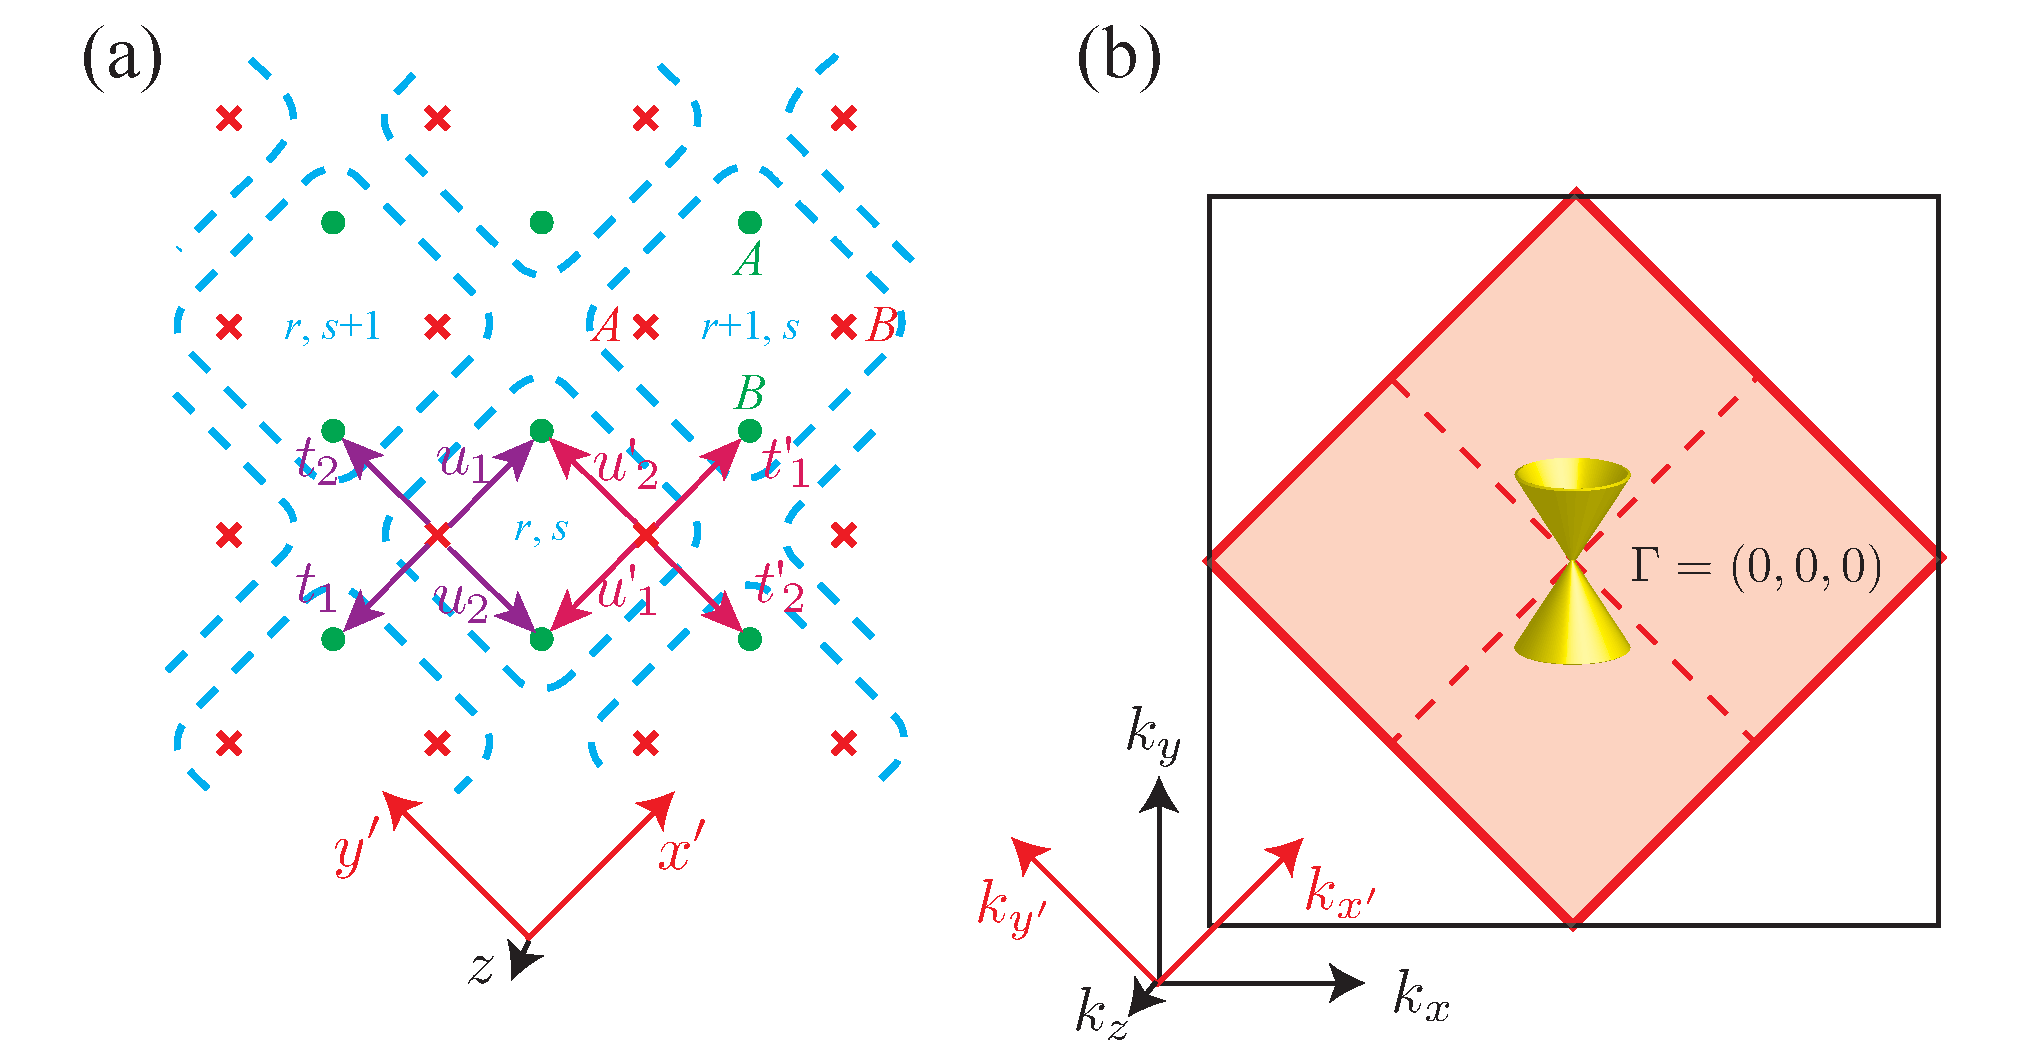
\includegraphics[width=0.9\textwidth]{DiracTB}
	\caption[(a) The massive AFTR and $C_2$ breaking coupled Dirac wire model. (b) The reduced Brillouin zone (BZ).]{(a) The massive AFTR and $C_2$ breaking coupled Dirac wire model. (b) The reduced Brillouin zone (BZ) after translation symmetry breaking where the two Weyl points collapse to a single Dirac point at $M$.}\label{fig:DiracTB}
	\centering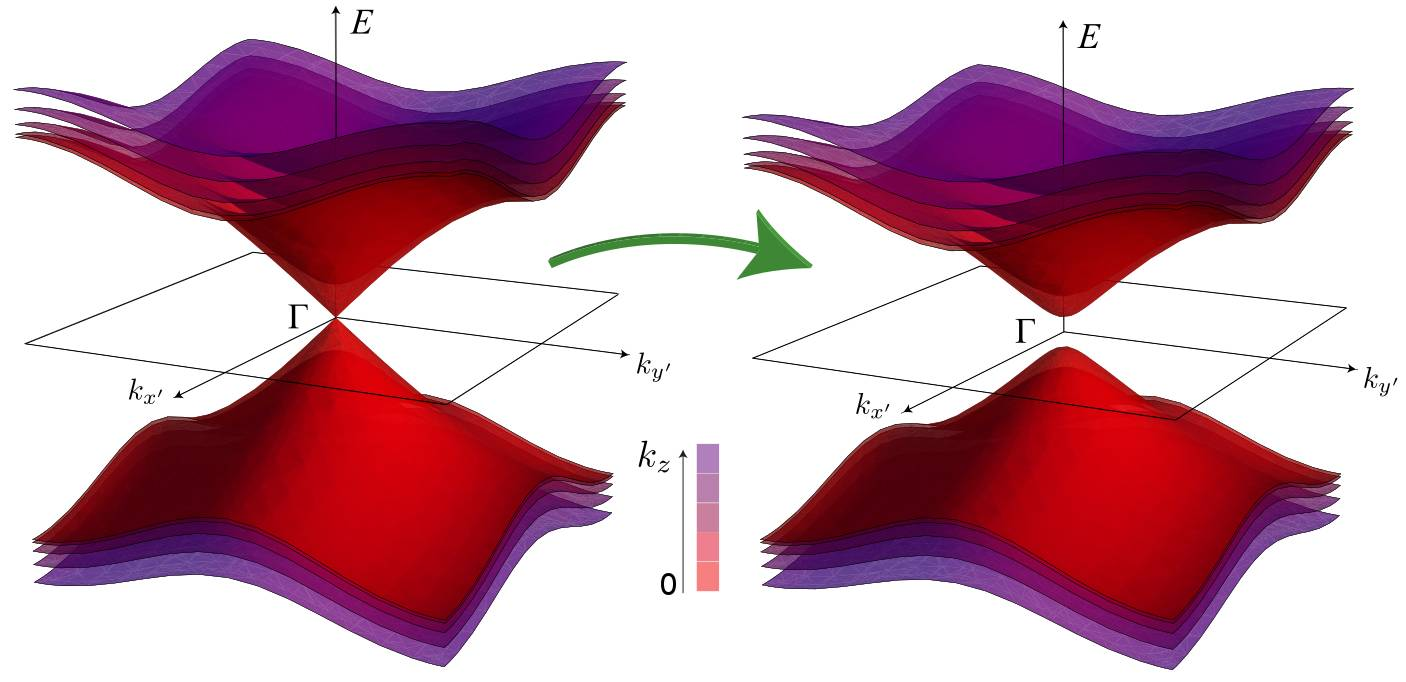
\includegraphics[width=0.96\textwidth]{Diracmassjpg.jpg}
	\caption{Dirac mass gap $2|\Delta|$ introduced by AFTR and $C_2$ symmetry breaking dimerization $\Delta=\Delta_1+i\Delta_2$.}\label{fig:Diracmassjpg}
\end{figure}

Remembering that the coupled wire model \eqref{WeylTBHam} (Fig.~\ref{fig:WeylTB}) descended from a vortex lattice of the microscopic parent Dirac Hamiltonian \eqref{DiracHam}, the Dirac mass $m({\bf r})$ actually allows the model to carry fewer symmetries than the low-energy effective Hamiltonian \eqref{WeylTBHam} suggests. Now that the translation symmetry is lowered, the \BZ is reduced (see Fig.~\ref{fig:DiracTB}(b)) so that the two Weyl points now coincide at the origin $\Gamma$. This recovers an unanomalous Dirac semimetallic model \eqref{DiracHam0} around $(k_{x'},k_{y'})=(0,0)$. The fourfold degenerate Dirac point is protected and pinned at $\Gamma$ due to the remaining \AFTR symmetry $\mathcal{T}_{11}$ -- which takes the role of a spinful time reversal ($\hat{T}^2=-1$) in the continuum limit -- and the $C_2$ (screw) symmetry about the $z$-axis. However, if any of these symmetries is further broken, the fourfold degeneracy of the Dirac point is not protected (c.f.~the original continuum Dirac model \eqref{DiracHam}). Figure~\ref{fig:DiracTB}(a) shows a dimerized coupled Dirac wire model that introduces a finite mass for the Dirac fermion. We label the Dirac fermion operators as $\psi_{r,s}^{\mu,\sigma}$, for $\sigma=\odot,\otimes$ the chirality, $\mu=A,B$ the new sublattice label, and $(r,s)$ label the coordinates of the unit cell according to the $45^\circ$-rotated $x',y'$-axes. \begin{align}\mathcal{H}'=&\sum_{r,s}\sum_{\mu=A,B}\hbar\tilde{v}\left({\psi_{r,s}^{\mu,\odot}}^\dagger k_z\psi_{r,s}^{\mu,\odot}-{\psi_{r,s}^{\mu,\otimes}}^\dagger k_z\psi_{r,s}^{\mu,\otimes}\right)\nonumber\\&+iu_1{\psi_{r,s}^{A,\odot}}^\dagger\psi_{r,s}^{A,\otimes}-iu'_1{\psi_{r,s}^{B,\odot}}^\dagger\psi_{r,s}^{B,\otimes}+h.c.\nonumber\\&-u_2{\psi_{r,s}^{B,\odot}}^\dagger\psi_{r,s}^{A,\otimes}+u'_2{\psi_{r,s}^{A,\odot}}^\dagger\psi_{r,s}^{B,\otimes}+h.c.\label{DiracTBHam}\\&-it_1{\psi_{r-1,s}^{A,\odot}}^\dagger\psi_{r,s}^{A,\otimes}+it'_1{\psi_{r+1,s}^{B,\odot}}^\dagger\psi_{r,s}^{B,\otimes}+h.c.\nonumber\\&+t_2{\psi_{r,s+1}^{B,\odot}}^\dagger\psi_{r,s}^{A,\otimes}-t'_2{\psi_{r,s-1}^{A,\odot}}^\dagger\psi_{r,s}^{B,\otimes}+h.c.\nonumber \,.\end{align} For instance, the model is identical to the \AFTR and $C_2$ symmetric one in \eqref{WeylTBHam} when $t_j=t'_j=u_j=u'_j$ for $j=1,2$. However, when the symmetries are broken, these hopping parameters do not have to agree.

The Bloch band Hamiltonian after Fourier transformation is \begin{gather}H({\bf k})=\left(\begin{array}{*{20}c}\hbar\tilde{v}k_z&h(k_{x'},k_{y'})\\h(k_{x'},k_{y'})^\dagger&-\hbar\tilde{v}k_z\end{array}\right),\label{DiracBloch}\\h(k_{x'},k_{y'})=\left(\begin{array}{*{20}c}iu_1-it_1e^{-ik_{x'}}&u'_2-t'_2e^{-ik_{y'}}\\-u_2+t_2e^{ik_{y'}}&-iu'_1+it'_1e^{ik_{x'}}\end{array}\right)\nonumber \,, \end{gather} where the $2\times2$ identity matrix and $h(k_{x'},k_{y'})$ acts on the sublattice $\mu=A,B$ degrees of freedom, and $-\pi\leq k_{x'},k_{y'}\leq\pi$ are the rotated momenta. We perturb about the Dirac fixed point by introducing the dimerizations $\Delta_j$ \begin{align}t_j=t'_j=u_j-\Delta_j=u'_j-\Delta_j\end{align} for $j=1,2$. About the $\Gamma=(0,0,0)$ point, \begin{align}H(\Gamma+\delta{\bf k})=&\hbar\tilde{v}\delta k_z\sigma_z-t_1\delta k_{x'}\sigma_x-t_2\delta k_{y'}\sigma_y\mu_x\nonumber\\&-\Delta_1\sigma_y\mu_z+\Delta_2\sigma_y\mu_y+O(\delta k^2).\label{DiracHamwire}\end{align} See Fig.~\ref{fig:Diracmassjpg} for its massive spectrum.

\begin{figure}[htbp]
	\centering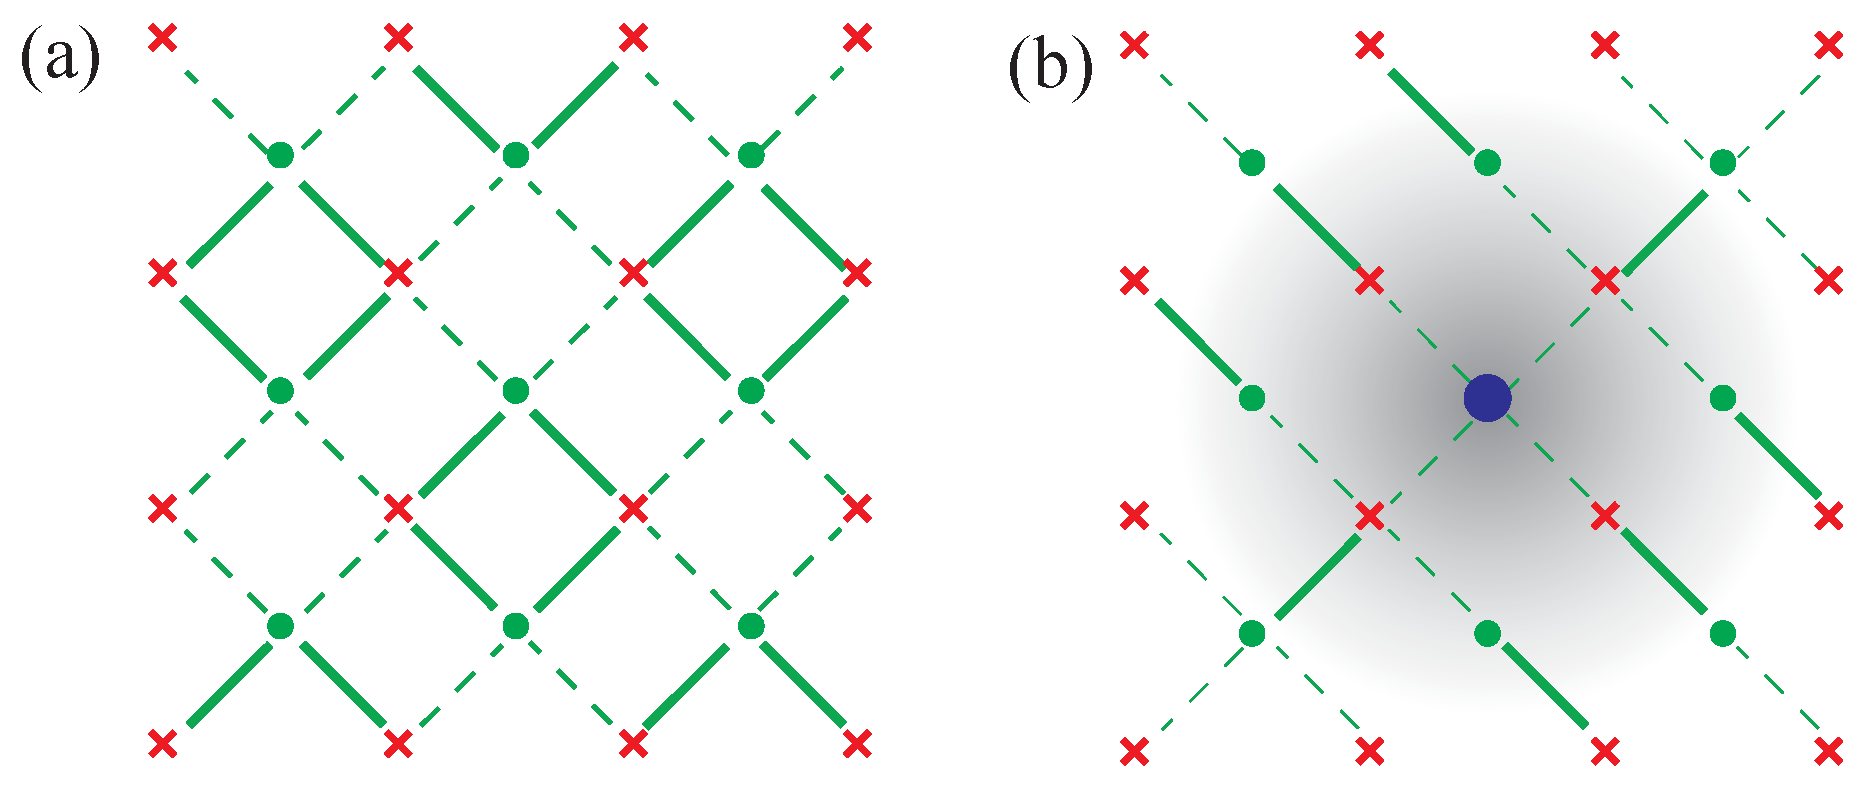
\includegraphics[width=0.8\textwidth]{dimerization}
	\caption[(a) Dimerized model of a massive Dirac fermion. (b) Vortex of dimerizations.]{(a) Dimerized model of a massive Dirac fermion. (b) Vortex of dimerizations $\Delta=\Delta_1+i\Delta_2$ that leaves behind a massless localized chiral Dirac channel (blue dot).}\label{fig:dimerization}
\end{figure}

Here the \AFTR symmetry $\mathcal{T}_{11}$ and the twofold rotation $\mathcal{C}_2$ are represented in the single-body picture by \begin{align}T_{11}({\bf k})&=\left(\begin{smallmatrix}0&0&-e^{ik_x}&0\\0&0&0&-1\\1&0&0&0\\0&e^{ik_x}&0&0\end{smallmatrix}\right)\mathcal{K},\nonumber\\C_2({\bf k})&=\left(\begin{smallmatrix}i&0&0&0\\0&ie^{-i(k_x+k_y)}&0&0\\0&0&-ie^{-ik_x}&0\\0&0&0&-ie^{-ik_y}\end{smallmatrix}\right)\end{align} (again suppressing the $C_2$ screw phase $e^{-ik_za/2}$ in the continuum limit $a\to0$). In the small $k_x,k_y$-limit, $T_{11}(0)=-i\sigma_y\mathcal{K}$ and $C_2(0)=i\sigma_z$. It is straightforward to check that the dimerization $\Delta_2$ preserves $\mathcal{T}_{11}$ while both $\Delta_1,\Delta_2$ breaks $C_2$.

Since the coupled wire model \eqref{DiracHamwire} and the parent continuum Dirac model \eqref{DiracHam} have the same matrix and symmetry structure, we can apply the same construction we discussed before to the new coarse-grained model \eqref{DiracHamwire}. For instance, the non-competing dimerizations $\Delta({\bf r})=\Delta_1({\bf r})+i\Delta_2({\bf r})$ can spatially modulate and form vortices in a longer length scale. Figure~\ref{fig:dimerization}(b) shows a dimerization pattern that corresponds to a single vortex in $\Delta$. The solid (dashed) lines represent strong (resp.~weak) backscattering amplitudes. In the fully dimerized limit where the dashed bonds vanish, all Dirac channels are gapped except the one at the center (showed as a blue dot). In the weakly dimerized case, there is a collective chiral Dirac channel whose wave function is a superposition of the original channels and is exponentially localized at the $\Delta$-vortex core, but now with a length scale longer than that of the original $m$-vortex lattice. These collective chiral Dirac $\Delta$-vortices can themselves form a coupled array, like \eqref{WeylTBHam}, and give a Dirac semimetal of even longer length scale. The single-body coupled vortex construction is therefore a coarse-graining procedure that recovers equivalent emergent symmetries at each step. \begin{align}\begin{diagram}\mbox{Dirac semimetal}&\pile{\rTo^{\mbox{\small mass vortices}}\\\lTo_{\mbox{\small coupled wire model}}}&\mbox{chiral Dirac strings \,.}\end{diagram}\end{align}

\subsubsection{Holographic projection from 4D}\label{sec:holproj4D}
The coupled wire model \eqref{WeylTBHam} with two \AFTR axes can be supported by a weak topological insulator (\hypertarget{WTI}{WTI}) in four dimensions. Instead of realizing the chiral Dirac channels using mass vortices of a 3D Dirac semimetal, they can be generated as edge modes along the boundaries of 2D Chern insulators (or lowest Landau levels). The 4D \WTI is constructed by stacking layers of Chern insulators parallel to the $zw$-plane along the $x$ and $y$ directions. The Chern layers $L_{\bf r}$, labeled by the checkerboard lattice vector ${\bf r}=r_x{\bf e}_x+r_y{\bf e}_y$ on the $xy$-plane, have alternating orientations so that $\mathrm{Ch}[L_{\bf r}]=1$ if $r_x,r_y$ are integers and $\mathrm{Ch}[L_{\bf r}]=-1$ if $r_x,r_y$ are half-integers.  The model therefore carries both \AFTR symmetries $\mathcal{T}_{11}$ and $\mathcal{T}_{\bar{1}1}$ as well as the $C_2$ rotation about $zw$, and when cleaved along a 3D hyper-surface normal to $w$, it generates the array of alternating chiral Dirac channels in Fig.~\ref{fig:WeylTB}.

The 4D \WTI model can also be regarded as a stack of 3D antiferromagnetic topological insulators (\hypertarget{AFTI}{AFTI})~\cite{MongEssinMoore10}. Restricting to the 3D hyperplane normal to $-{\bf e}_x+{\bf e}_y$, this model consists of alternating Chern insulating layers parallel to the $wz$-plane stacked along the ${\bf e}_x+{\bf e}_y$ direction. This 3D model describes an \AFTI with a non-trivial $\mathbb{Z}_2$ index. For instance along the boundary surfaces normal to $w$ or $z$ that preserve the antiferromagnetic symmetry $\mathcal{T}_{11}$, the model leaves behind a 2D array of alternating chiral Dirac wires. The uniform nearest wire backscattering term $t_1$ (see \eqref{WeylTBHam}) introduces a linear dispersion along the $11$-direction and gives rise to a single massless surface Dirac cone spectrum at a \TRIM on the boundary of the surface \BZ where $\mathcal{T}_{11}^2=-1$. The 4D \WTI model is identical to stacking these 3D \AFTI along the $\bar{1}1$-off-diagonal direction $-{\bf e}_x+{\bf e}_y$. 

\subsection{Surface Fermi arcs}\label{sec:fermiarc1}

\subsubsection{AFTR breaking surfaces}\label{sec:fermiarcAFTRbreaking}

\begin{figure}[htbp]
	\centering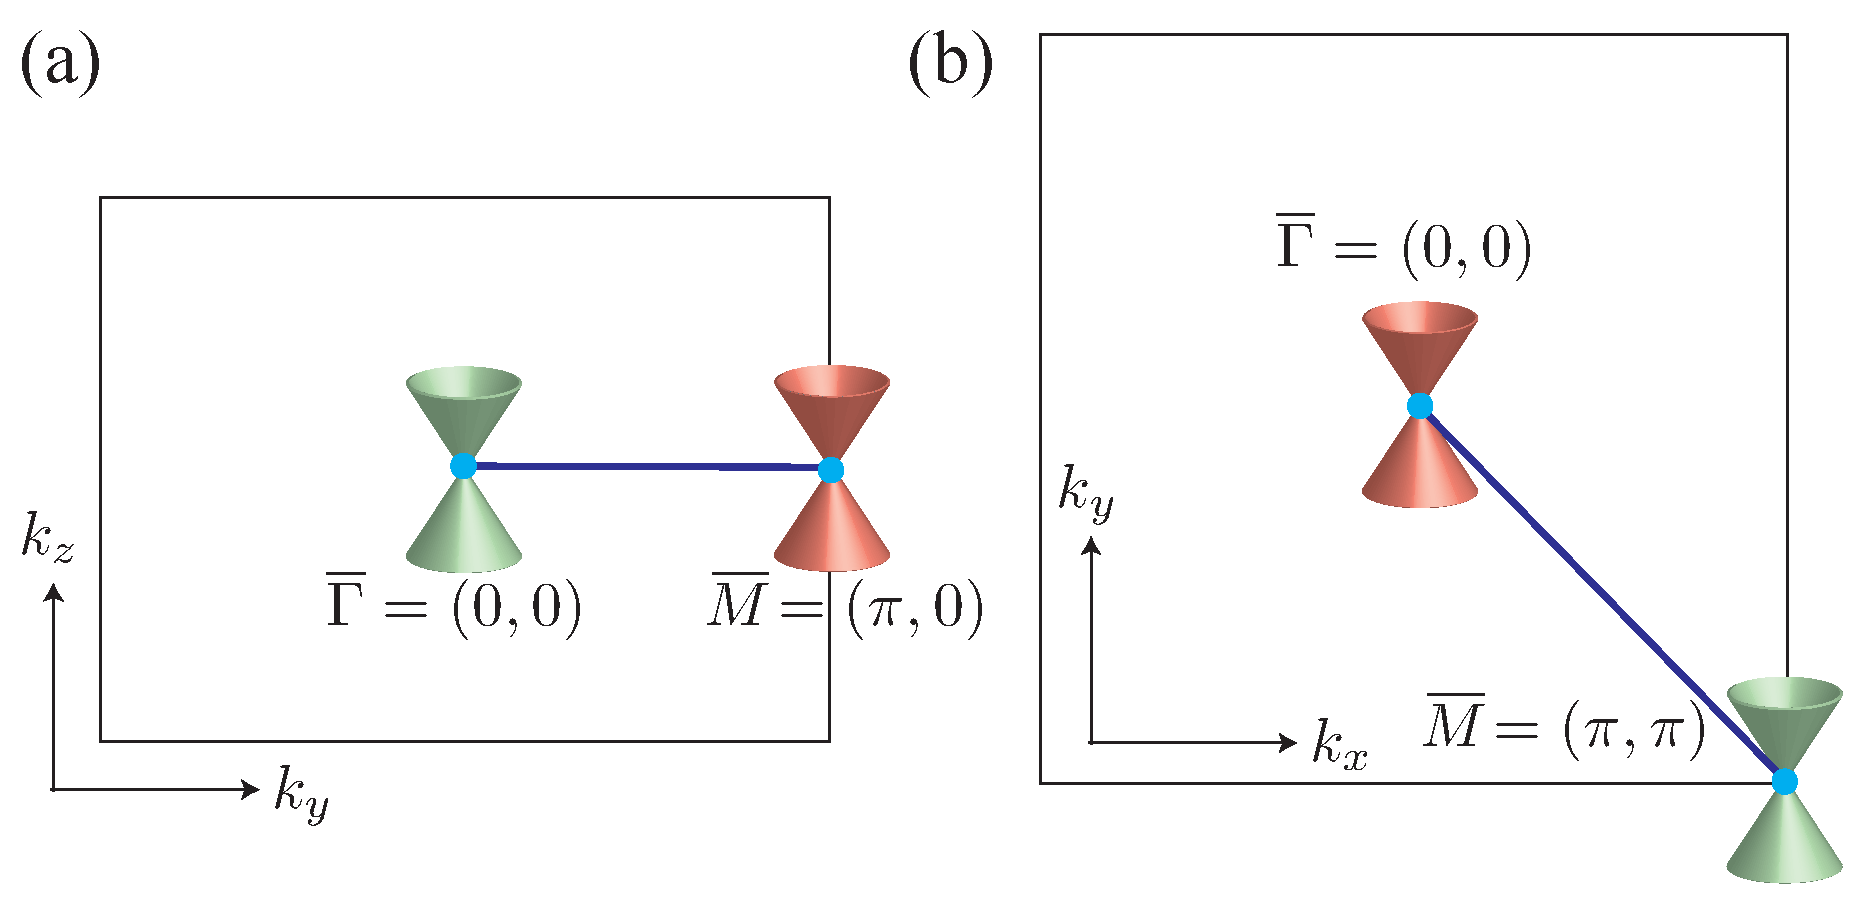
\includegraphics[width=0.8\textwidth]{fermiarc1}
	\caption[Fermi arcs joining projected Weyl points on the surface Brillouin zones]{Fermi arcs (blue lines) joining projected Weyl points on the surface Brillouin zones along (a) the $(100)$ surface and (b) the $(001)$ surface.}\label{fig:fermiarc1}
\end{figure}
We discuss the surface states of the coupled Dirac wire model \eqref{WeylTBHam}. Similar to the boundary surface of a translation symmetry protected Dirac semimetal (or more commonly called a Weyl semimetal), there are Fermi arcs connecting the surface-projected Weyl points~\cite{WanVishwanathSavrasovPRB11,Ashvin_Weyl_review,RMP}. First we consider the $(100)$ surface normal to $x$-axis (see Fig.~\ref{fig:WeylTB}). We assume the boundary cuts between unit cells and set the Fermi energy at $\varepsilon_f=0$. At $k_z=0$ and given a fixed $k_y\in(-\pi,\pi)$, the tight-binding model \eqref{BlochHam} is equivalent to the Su-Schriffer-Heeger model~\cite{SSH} or a 1D class AIII topological insulator~\cite{SchnyderRyuFurusakiLudwig08,Kitaevtable08} along the $x$-direction protected by the chiral symmetry $\sigma_zH(k_x)=-H(k_x)\sigma_z$. It is characterized by the winding number \begin{align}w(k_y)&=\frac{i}{2\pi}\int_{-\pi}^\pi \frac{1}{g(k_x,k_y)}\frac{\partial g(k_x,k_y)}{\partial k_x}dk_x \,, \\&=\left(1+\mathrm{sgn}(k_y t_1/t_2)\right)/2.\nonumber\end{align} When $t_1,t_2$ have the same (or opposite) sign, the quasi-1D model is topological along the positive (resp.~negative) $k_y$-axis and thus carries a boundary zero mode. This corresponds to the Fermi line joining the two surface projected Weyl points at $\overline{\Gamma}$ and $\overline{M}$ (see Fig.~\ref{fig:fermiarc1}(a)). As the zero modes have a fixed chirality according to $\sigma_z$, they propagate uni-directionally with the dispersion $E(k_z)=\hbar\tilde{v}k_z\sigma_z$. The cleaving surface breaks \AFTR and $C_2$ symmetries, and so does the Fermi arc in Fig.~\ref{fig:fermiarc1}(a). For instance, any one of the \AFTR symmetries maps the boundary surface to an inequivalent one that cuts through unit cells instead of between them. As a result, the Fermi arc will connect the Weyl points along the opposite side of the $k_y$-axis for this surface. 

The $(010)$ surface Fermi arc structure is qualitatively equivalent to that of the $(100)$ surface. The $(110)$ and $(1\bar{1}0)$ surfaces that cleave along the diagonal and off-diagonal axes (see Fig.~\ref{fig:WeylTB}) respectively preserve the \AFTR symmetries $\mathcal{T}_{11}$ and $\mathcal{T}_{\bar{1}1}$. There are no protected surface Fermi arcs because the two bulk Weyl points project onto the same point on the surface Brillouin zone. Lastly, we consider the $(001)$ surface normal to the $z$-axis, which is the direction of the chiral Dirac strings that constitute the coupled wire model. A chiral Dirac channel cannot terminate on the boundary surface. In a single-body theory, it must bend and connect with an adjacent counter-propagating one. Although the $(001)$ plane is closed under the $C_2$ as well as both the \AFTR symmetries, the surface bending of Dirac channels must violate at least one of them. Here we consider the simplest case where the counter-propagating pair of Dirac channels within a unit cell re-connects on the boundary surface. This boundary is equivalent to a domain wall interface separating the Dirac semimetal \eqref{WeylTBHam} from an insulator where Dirac channels backscatters to their counter-propagating partner within the same unit cell. 

The domain wall Hamiltonian takes the form of a differential operator
\begin{align}\hat{\mathcal{H}}=&\sum_{m,j}-i\hbar\tilde{v}\left({\psi_{m,j}^\odot}^\dagger\partial_z\psi_{m,j}^\odot-{\psi_{m,j}^\otimes}^\dagger\partial_z\psi_{m,j}^\otimes\right)\label{WeylTBHamwall}\\&+it_1\left({\psi_{m,j}^\odot}^\dagger\psi_{m,j}^\otimes+\theta(z){\psi_{m-1,j-1}^\odot}^\dagger\psi_{m,j}^\otimes\right)+h.c.\nonumber\\&+t_2\theta(z)\left({\psi_{m-1,j}^\odot}^\dagger\psi_{m,j}^\otimes+{\psi_{m,j-1}^\odot}^\dagger\psi_{m,j}^\otimes\right)+h.c.\nonumber\end{align} by replacing $k_z\leftrightarrow-i\partial_z$ in \eqref{WeylTBHam}. Here $\theta(z)$ can be the unit step function or any function that asymptotically approaches 1 for $z\to\infty$ or 0 for $z\to-\infty$. The model therefore describes the Dirac semimetal \eqref{WeylTBHam} for positive $z$, and an insulator for negative $z$ where Dirac channels are pair annihilated within a unit-cell by $t_1$. After a Fourier transformation, the Bloch Hamiltonian $\hat{H}(k_x,k_y)$ is identical to \eqref{BlochHam} by replacing $k_z\leftrightarrow-i\partial_z$ and $g(k_x,k_y,z)=it_1(1+\theta(z)e^{-i(k_y+k_x)})+t_2\theta(z)(e^{-ik_x}+e^{-ik_y})$. Given any fixed $k_x,k_y$, the differential operator $\hat{H}(k_x,k_y)$ is identical to the Jackiw-Rebbi model~\cite{JackiwRebbi76}. Deep in the insulator, $g(k_x,k_y,z\to-\infty)=it_1$. There is an interface zero mode at the surface domain wall if $g$ changes sign, i.e.~if $g(k_x,k_y,z\to\infty)=|g|e^{i\varphi}$ has argument $\varphi=-\mathrm{sign}(t_1)\pi/2$. When $\varepsilon_f=0$, the zero modes trace out a Fermi arc that connects the two surface projected Weyl points (see Fig.~\ref{fig:fermiarc1}(b)).

\begin{figure}[htbp]\centering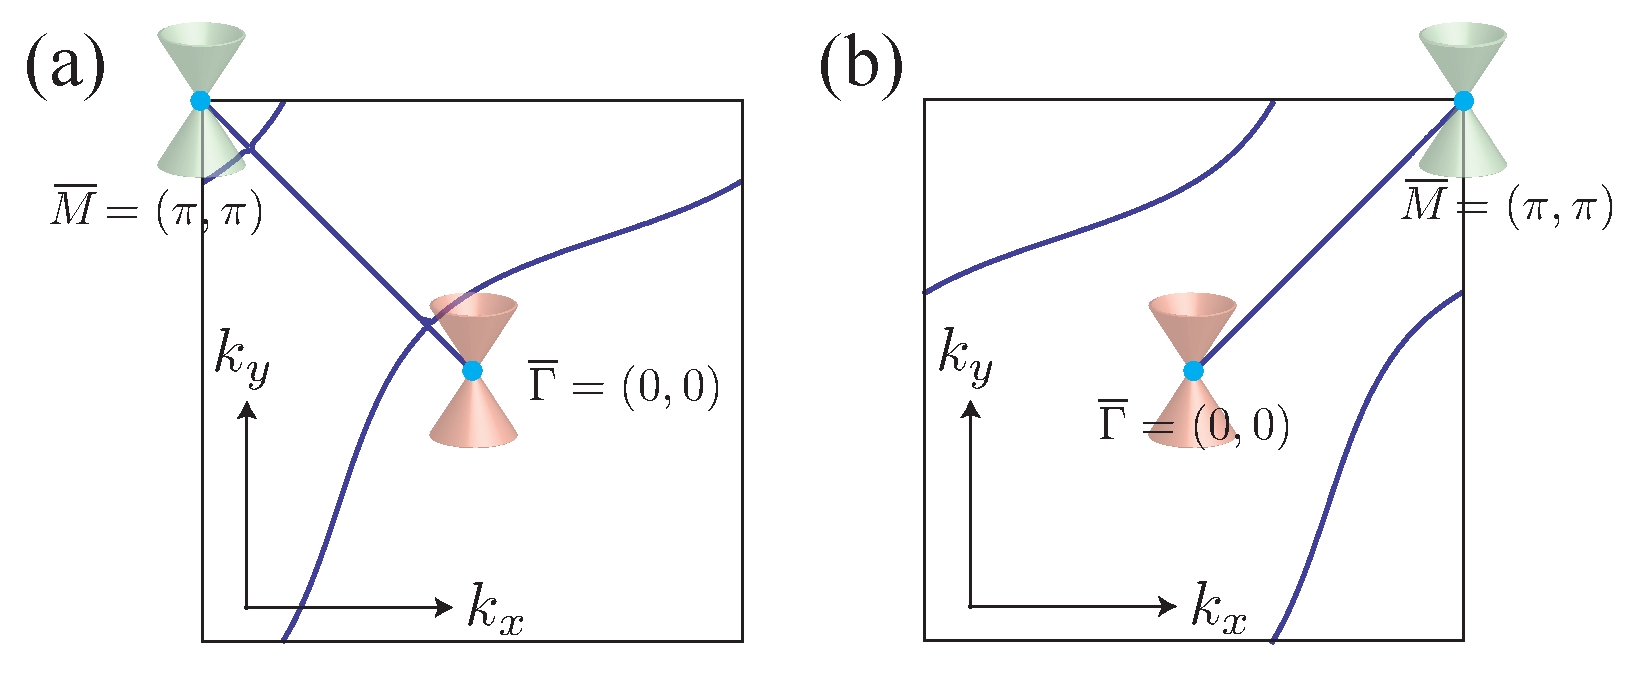
\includegraphics[width=0.8\textwidth]{fermiarc2}\caption[Fermi arcs on the $(001)$ surface with alternative boundary conditions]{Fermi arcs (blue lines) on the $(001)$ surface with alternative boundary conditions (a) $g(k_x,k_y)=-it_1$ and (b) $g(k_x,k_y)=-t_2e^{-ik_y}$ in the insulating domain, for $t_2/t_1=2$.}\label{fig:fermiarc2}\end{figure}

We notice that in the insulating phase (or on the boundary surface), Dirac wires can be backscattered with a different phase and dimerized out of the unit cell. These different boundary conditions correspond to distinct surface Fermi arc patterns. Figure~\ref{fig:fermiarc2} shows two alternatives. (a) shows the zero energy arcs when intra-cell backscattering reverses sign $t_1\to-t_1$ in the insulating domain. (b) shows a case when the dimerization is taken along the off-diagonal axis. These inequivalent boundary conditions differ by some three dimensional integer quantum Hall states, which correspond to additional chiral Fermi arcs that wrap non-trivial cycles around the 2D toric surface Brillouin zone.

\subsubsection{AFTR preserving surfaces}\label{sec:fermiarcAFTRpreserving}

We also notice that the Fermi arc structures in Figs.~\ref{fig:fermiarc1}(b) and \ref{fig:fermiarc2} are allowed because both the \AFTR symmetries $\mathcal{T}_{11}$, $\mathcal{T}_{\bar{1}1}$ and the $C_2$ symmetry are broken by the insulating domain. Any dimerization that preserves only one of $\mathcal{T}_{11}$ and $\mathcal{T}_{\bar{1}1}$ necessarily breaks translation symmetry, and corresponds to an enlarged unit cell and a reduced Brillouin zone (c.f.~Fig.~\ref{fig:Chernstack} and \ref{fig:DiracTB}). As a result, the two Weyl points would now collapse onto the same $\overline{\Gamma}$ point. Any momentum plane that contains the $k_z$-direction and avoids the $\Gamma$ point must have trivial Chern invariant, because it could always be deformed (while containing the $k_z$-direction and avoiding the $\Gamma$ point) to the reduced Brillouin zone boundary, where its Chern invariant would be killed by the \AFTR symmetry. %There would therefore be no protected surface Fermi arcs.

However, the trivial bulk Chern invariant does not imply the absence of surface state. This can be understood by looking at the surface boundary in real space. Here, we assume the Dirac strings that constitute the coupled wire model \eqref{WeylTBHam} are supported by vortices of an underlying Dirac mass (see Fig.~\ref{fig:vortexlattice} and eq.\eqref{DiracHam}). The semimetallic coupled wire model terminates along the $xy$-plane against vacuum, which is modeled by the Dirac insulator $H_{\mathrm{vacuum}}=\hbar v{\bf k}\cdot\vec{s}\mu_z+m_0\mu_x$, say with $m_0>0$. Recall from \eqref{massT11} that the Dirac mass vortex configuration \eqref{Jacobielliptic} is \AFTR symmetric along the $\mathcal{T}_{11}$-directions. The Dirac insulating vacuum is symmetric under local \TR as well as continuous translation. It however breaks the screw rotation symmetry $\hat{C}_2=is_z\mu_z$, but we here only focus on the \AFTR symmetry.

\begin{figure}[htbp]
	\centering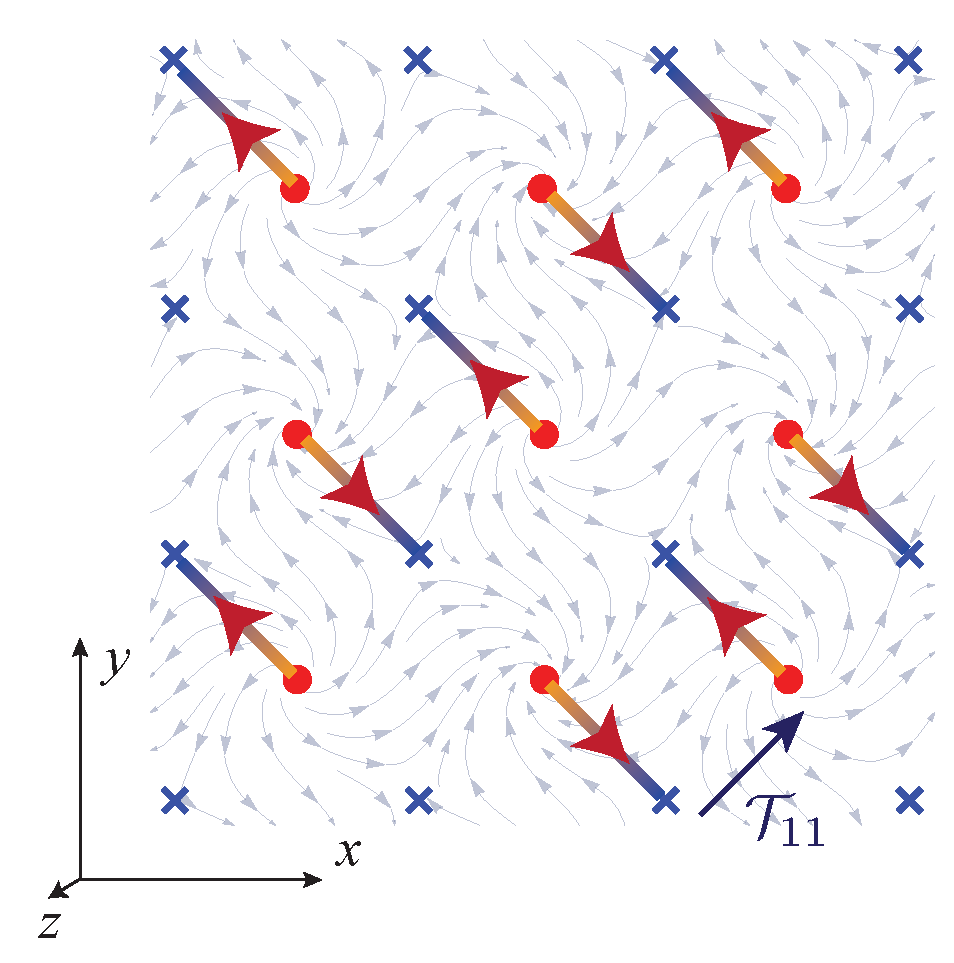
\includegraphics[width=0.6\textwidth]{SurfaceStates1bdy}
	\caption{Surface chiral Dirac channels of the coupled wire model \eqref{WeylTBHam} terminated along the $xy$ plane.}\label{fig:SurfaceStates1bdy}
\end{figure}

The surface boundary supports chiral Dirac channels that connect the chiral Dirac strings in the semimetallic bulk that are normal to the surface. The surface channels are shown in Fig.~\ref{fig:SurfaceStates1bdy}. The {\color{blue}$\times$} ({\color{red}$\bullet$}) represent chiral vortices in the bulk that direct electrons away from (resp.~onto) the surface. The vector field represents the Dirac mass $m({\bf r})=m_x({\bf r})+im_y({\bf r})$ modulation in the semimetallic bulk near the surface. The surface Dirac line channels~\cite{TeoKane} -- shown by directed lines connecting the bulk Dirac strings {\color{blue}$\times$}, {\color{red}$\bullet$} -- are located where the \TR symmetric Dirac mass $m_x$ changes sign across the surface boundary and the \TR breaking Dirac mass $m_y$ flips sign across the line channels along the surface. In other words, they are traced out of points on the surface where $m_x<0$ and $m_y=0$. Each of these surface channels carries a chiral Dirac electronic mode that connects the bulk chiral Dirac vortices. They can couple through inter-channel electron tunneling, but the collective gapless surface state cannot be removed from low-energy by dimerization without breaking the \AFTR symmetry $\mathcal{T}_{11}$. %The surface state is, in a sense, half of that of a weak topological insulator (or 3D stack of quantum spin Hall layers). 


\section{Many-body interacting variations}\label{sec:intenable}

We discuss the effect of strong many-body interactions in a Dirac semimetal in three dimensions. Before we do so, it is worth stepping back and reviewing the two dimensional case in order to illustrate the issue and idea that will be considered and generalized in three dimensions. The massless Dirac fermion with $H=\hbar v(k_xs_y-k_ys_x)$ that appears on the surface of a topological insulator~\cite{HasanKane10,QiZhangreview11,HasanMoore11,RMP} is protected by time reversal (TR) and charge $U(1)$ symmetries and is anomalous. This means that there is no single-body energy gap opening mass term that preserves the symmetries, and there is no single-body fermionic lattice model in two dimensions that supports a massless Dirac fermion without breaking the symmetries. Neither of these statements hold true in the many-body setting. The surface Dirac fermion can acquire a \TR and charge $U(1)$ preserving many-body interacting mass.~\cite{WangPotterSenthilgapTI13,ChenFidkowskiVishwanath14,MetlitskiKaneFisher13b,BondersonNayakQi13} Consequently, this also enables a massless symmetry preserving Dirac fermion in a pure 2D system without holographically relying on a semi-infinite 3D topological bulk. For instance, one can take a quasi-2D topological insulator slab with finite thickness and remove the Dirac fermion on one of the two surfaces by introducing an interacting mass gap. This leaves a single massless Dirac fermion on the opposite surface without breaking symmetries.

A massless Dirac fermion in three dimensional semimetallic materials can be protected in the single-body picture by screw rotation, time reversal and charge $U(1)$ symmetries (see reviews Ref.~\cite{Ashvin_Weyl_review,RMP,ArmitageMeleVishwanath16} and Sec.~\ref{sec:DiracSemimetal}). From a theory point of view, it can be supported on the 3D boundary of a 4D weak topological insulator, where the two Weyl fermions are located at distinct time reversal invariant momenta (recall Fig.~\ref{fig:Weylspectrum} and Sec.~\ref{sec:holproj4D} for the antiferromagnetic case). In this case, the massless fermions are protected by translation, time reversal and charge $U(1)$ symmetries. In this section, we address the following issues. (1) We show by explicitly constructing an exactly solvable coupled wire model that the 3D Dirac fermion can acquire a many-body interacting mass while preserving all symmetries. (2) We show in principle that an antiferromagnetic time reversal (AFTR) symmetric massless 3D Dirac system with two Weyl fermions separated in momentum space can be enabled by many-body interactions without holographically relying on a higher dimensional topological bulk.

We begin with the Dirac semimetallic coupled wire model in Fig.~\ref{fig:Weylspectrum} and \eqref{WeylTBHam}. In particular, we focus on many-body interactions that facilitate the fractionalization of a $(1+1)$D chiral Dirac channel \begin{align}\mathrm{Dirac}=\mathrm{Pfaffian}\otimes\mathrm{Pfaffian}\label{fractionalization}\end{align} (see also Fig.~\ref{fig:glueingsplitting}). In a sense, each chiral Pfaffian channel carries half of the degrees of freedom of the Dirac. For instance, it has half the electric and thermal conductances, which are characterized by the filling fraction $\nu=1/2$ and the chiral central charge $c=1/2$ in \eqref{conductance}. Throughout this dissertation, we refer to the low-energy effective \CFT -- that consists of an electrically charged $U(1)_4$ bosonic component, say moving in the $R$ direction, and a neutral Majorana fermion component moving in the opposite $L$ direction -- simply as a Pfaffian \CFT \begin{align}\mathrm{Pfaffian}=U(1)_4\otimes\overline{\mathrm{Ising}}.\label{PfaffianCFT}\end{align} (In this article, we follow the level convention for $U(1)$ in the \CFT community~\cite{bigyellowbook}. The same theory may be more commonly referred to as $U(1)_8$ in the fractional quantum Hall community. For clarification, see Lagrangian \eqref{Pfaffian} and \eqref{LFQHCS}.)

While this is not the focus of this article, here we clarify and disambiguate the three ``Pfaffian" fractional quantum Hall (\hypertarget{FQH}{FQH}) states that commonly appear in the literature. All these $(2+1)$D states are theorized at filling fraction $\nu=1/2$, although being applied to $\nu=5/2$ in materials, and have identical electric transport properties. However, they have distinct thermal Hall transport behaviors. They all have very similar anyonic quasiparticle (\hypertarget{QP}{QP}) structures. For instance, they all have four Abelian and two non-Abelian \QP (up to the electron). On the other hand, the charge $e/4$ non-Abelian Ising anyons of the three states have different spin-exchange statistics. First, the gapless boundary of the Moore-Read Pfaffian \FQH state~\cite{MooreRead,ReadMoore,GreiterWenWilczekPRL91,GreiterWenWilczek91} can be described by the $(1+1)$D chiral \CFT $U(1)_4\otimes\mathrm{Ising}$ where the charged boson and neutral fermion sectors are co-propagating. It therefore carries the chiral central charge $c=1+1/2=3/2$, which dictates the thermal Hall response \eqref{conductance}. Second, the ``anti-Pfaffian" \FQH state~\cite{LevinHalperinRosenow07,LeeRyuNayakFisher07} is the particle-hole conjugate of the Moore-Read Pfaffian state. Instead of half-filling the lowest Landau level by electrons, one can begin with the completely filled lowest Landau level, and half-fill it with holes. In a sense the anti-Pfaffian state is obtained by subtracting the completely filled lowest Landau level by a Moore-Read Pfaffian state. Along the boundary, the $(1+1)$D \CFT $U(1)_{1/2}\otimes\overline{U(1)_4\otimes\mathrm{Ising}}$ consists of the forward propagating chiral Dirac $U(1)_{1/2}$ sector that corresponds to the lowest Landau level, and the backward propagating Moore-Read Pfaffian $\overline{U(1)_4\otimes\mathrm{Ising}}$. Here $\overline{\mathcal{C}}$ can be interpreted as the time-reversal conjugate of the chiral \CFT $\mathcal{C}$. The thermal transport is governed by the edge chiral central charge $c=1-3/2=-1/2$, which has an opposite sign from the filling fraction. Thus, unlike the Moore-Read Pfaffian state, the net electric and thermal currents now travel in opposite directions along the edge. Lastly, the recently proposed particle-hole symmetric (\hypertarget{PHS}{PHS}) Pfaffian state~\cite{Son15,BarkeshliMulliganFisher15,WangSenthil16}, which is going to be the {\em only} Pfaffian \FQH state considered in this article (see Ref.~\cite{KaneSternHalperin17} for a coupled wire construction), has the chiral edge \CFT \eqref{PfaffianCFT}. As the electrically charged boson and neutral fermion sectors are counter-propagating, the net thermal edge transport is governed by the chiral central charge $c=1-1/2=1/2$. The chiral $(1+1)$D \PHS Pfaffian \CFT \eqref{PfaffianCFT} is also present along the line interface separating a \TR symmetric $\mathcal{T}$-Pfaffian~\cite{ChenFidkowskiVishwanath14} domain and a \TR breaking magnetic domain on the surface of a 3D topological insulator. (Similar constructions can be applied to alternative \TR symmetric topological insulator surface states~\cite{WangPotterSenthilgapTI13,MetlitskiKaneFisher13b,BondersonNayakQi13}, but they will not be considered in this article.) Other than their thermal transport properties, the three Pfaffian \FQH state can also be distinguished by the charge $e/4$ Ising anyon, which has spin $h=1/8$, $-1/8$ or $0$ for the Moore-Read Pfaffian, anti-Pfaffian or \PHS Pfaffian states respectively. 

Since we will not be considering the Moore-Read Pfaffian or its particle-hole conjugate anti-Pfaffian state, we will simply refer to the \PHS Pfaffian state as the Pfaffian state. The low-energy effective chiral $(1+1)$D \CFT takes the decoupled form between the boson and fermion \begin{align}\mathcal{L}_{\mathrm{Pfaffian}}&=\mathcal{L}_{\mathrm{charged}}+\mathcal{L}_{\mathrm{neutral}} \,, \label{Pfaffian}\\&=\frac{8}{2\pi}\partial_t\phi_R\partial_x\phi_R+v(\partial_x\phi_R)^2\nonumber\\&\;\;\;+i\gamma_L(\partial_t-\tilde{v}\partial_x)\gamma_L\nonumber \,, \end{align} where we have set $\hbar=1$. Here $\phi_R$ is the free chiral $U(1)_4$ boson. It generates the $(1+1)$D theory $\mathcal{L}_{\mathrm{charged}}$, which is identical to the boundary edge theory of the $(2+1)$D bosonic Laughlin $\nu=1/8$ fractional quantum Hall state described by the topological Chern-Simon theory~\cite{WenZee92,Wenedgereview} \begin{align}\mathcal{L}_{2+1}=\frac{K}{4\pi}\alpha\wedge d\alpha+et\alpha\wedge dA \,, \label{LFQHCS}\end{align} with $K=8$ and $t=2$. The $U(1)_4$ \CFT carries the electric conductance $\sigma=tK^{-1}t=1/2$ in units of $2\pi e^2=e^2/h$ and a thermal conductance characterized by the chiral central charge $c=c_R=1$. Primary fields are of the form of (normal ordered) chiral vertex operators $:e^{im\phi_R}:$, for $m$ an integer, and carries charge $q=m/4$ in units of $e$ and conformal scaling dimension (i.e.~conformal spin) $h=h_R=m^2/16$. We summarize and abbreviate the operator product expansion \begin{align}e^{im_1\phi_R(z)}e^{im_2\phi_R(w)}=e^{i(m_1+m_2)\phi_R(w)}(z-w)^{m_1m_2/8}+\ldots\end{align} by the Abelian fusion rule \begin{align}e^{im_1\phi_R}\times e^{im_2\phi_R}=e^{i(m_1+m_2)\phi_R},\end{align} where $z\sim\tau+ix$ is the complex space-time parameter and $\tau=i\pi vt/2$ is the Euclidean time.

$\gamma_L^\dagger=\gamma_L$ is the free Majorana fermion. It generates the $(1+1)$D theory $\mathcal{L}_{\mathrm{neutral}}$, which is equivalent to a chiral component of the critical Ising \CFT or the boundary edge theory of the $(2+1)$D Kitaev honeycomb model~\cite{Kitaev06} in its B-phase with \TR breaking (i.e.~a chiral $p_x+ip_y$ superconductor coupled with a $\mathbb{Z}_2$ gauge theory). It carries trivial electric conductance but contributes to a finite thermal conductance characterized by the chiral central charge $c=-c_L=-1/2$. The Ising \CFT has primary fields $1$, $\gamma_L$ and $\sigma_L$, where the twist field (or Ising anyon) $\sigma_L$ carries the conformal spin $h=-h_L=-1/16$. Again, we abbreviate the operator product expansions \begin{gather}\gamma_L(\bar{z})\gamma_L(\bar{w})=\frac{1}{\bar{z}-\bar{w}}+\ldots\nonumber \,, \\\sigma_L(\bar{z})\gamma_L(\bar{w})=\frac{\sigma_L(\bar{w})}{(\bar{z}-\bar{w})^{1/2}}+\ldots\nonumber \,, \\\sigma_L(\bar{z})\sigma_L(\bar{w})=\frac{1}{(\bar{z}-\bar{w})^{1/8}}+(\bar{z}-\bar{w})^{3/8}\gamma_L(\bar{w})\nonumber \end{gather} by the fusion rule \begin{gather}\gamma_L\times\gamma_L=1,\quad\sigma_L\times\gamma_L=\sigma_L\nonumber \,, \\\sigma_L\times\sigma_L=1+\gamma_L,\end{gather} where $\bar{z}\sim\tau-ix$ is the complex space-time parameter and $\tau=i\tilde{v}t$ is the Euclidean time. 

General primary fields of the Pfaffian \CFT decompose into the $U(1)_4$ part and the Ising part. They take the form \begin{align}1_m=e^{im\phi_R},\quad\psi_m=e^{im\phi_R}\gamma_L,\quad\sigma_m=e^{im\phi_R}\sigma_L.\label{Pfaffianfields}\end{align} The conformal spins and fusion rules also decompose so that \begin{align}h_{1_m}=\frac{m^2}{16},\quad h_{\psi_m}=\frac{m^2}{16}+\frac{1}{2},\quad h_{\sigma_m}=\frac{m^2-1}{16}\end{align} modulo 1, $q_m=m/4$ in units of $e$, and \begin{gather}1_{m_1}\times1_{m_2}=\psi_{m_1}\times\psi_{m_2}=1_{m_1+m_2}\nonumber \,, \\1_{m_1}\times\psi_{m_2}=\psi_{m_1+m_2}\nonumber \,, \\1_{m_1}\times\sigma_{m_2}=\psi_{m_1}\times\sigma_{m_2}=\sigma_{m_1+m_2}\nonumber \,, \\\sigma_{m_1}\times\sigma_{m_2}=1_{m_1+m_2}+\psi_{m_1+m_2}.\end{gather} The $2\pi$ monodromy phase $\mathcal{M}^{XY}_Z=R^{XY}_ZR^{YX}_Z$ between primary fields $X$ and $Y$ with a fixed overall fusion channel $Z$ can be deduced by the {\em ribbon identity}~\cite{Kitaev06} \begin{align}e^{2\pi ih_Z}=\vcenter{\hbox{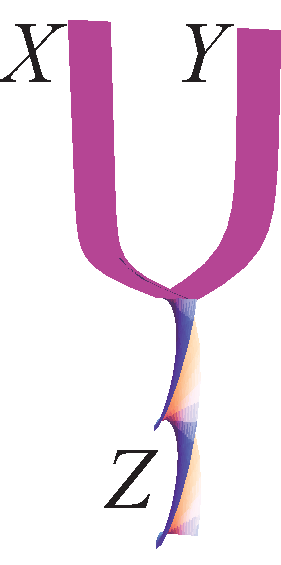
\includegraphics[width=0.5in]{ribbon1.pdf}}}=\vcenter{\hbox{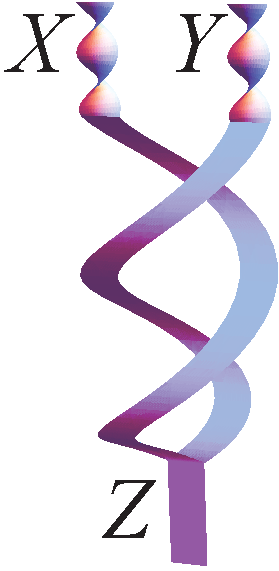
\includegraphics[width=0.5in]{ribbon2.pdf}}}=\mathcal{M}^{XY}_Ze^{2\pi i(h_X+h_Y)}\label{ribbonapp}\end{align} for $h_{X,Y,Z}$ the conformal spins for primary fields $X,Y,Z$. Unlike the gauge dependent $\pi$-exchange phase $R^{XY}_Z$, the $2\pi$-monodromy phase $\mathcal{M}^{XY}_Z=e^{2\pi i(h_Z-h_X-h_Y)}$ is gauge independent and physical.

The electronic quasiparticle is the composition $\psi_{\mathrm{el}}=e^{-i4\phi_R}\gamma_L$ so that it is fermionic and has electric charge $-1$ in units of $e$. Since electron is the fundamental building block of the system, locality of $\psi_{\mathrm{el}}$ only allows primary fields $X$ that have trivial monodromy $\mathcal{M}^{X,\psi_{\mathrm{el}}}=1$ with the electron. As a result, this restricts $1_m,\psi_m$ to even $m$ and $\sigma_m$ to odd $m$. Lastly, the coupled wire models constructed later will involve the Pfaffian channels that propagate in both forward and backward directions. We will denote the backward case by $\overline{\mathrm{Pfaffian}}$, whose Lagrangian density is the time reversal of \eqref{Pfaffian}, i.e.~replacing $R\leftrightarrow L$, $i\leftrightarrow-i$ and $\partial_t\leftrightarrow-\partial_t$. 

\subsection{Gluing and splitting}\label{sec:gluing}

\begin{figure}[htbp]
	\centering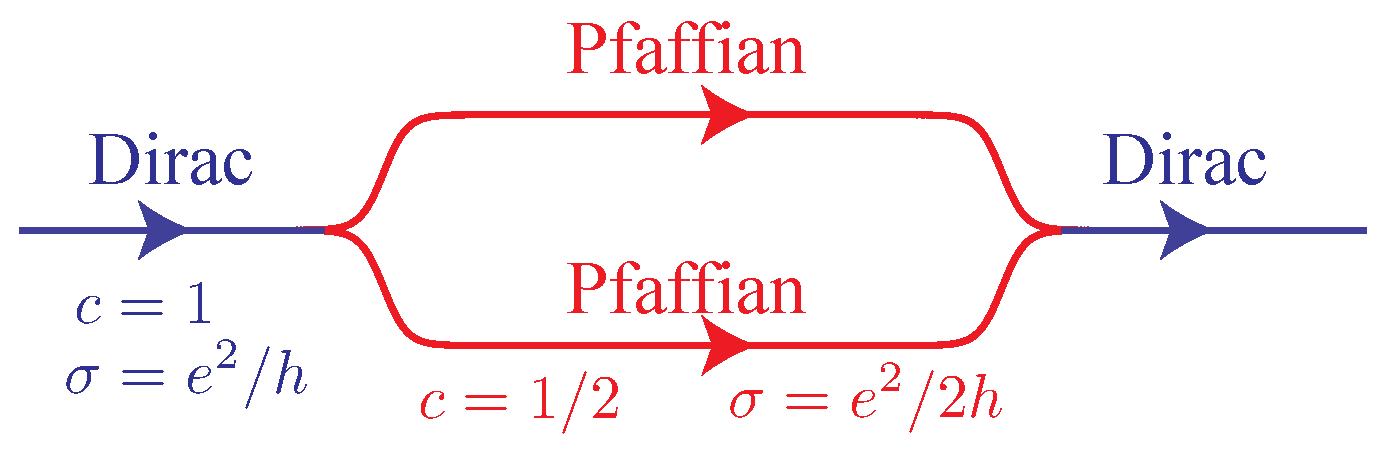
\includegraphics[width=0.6\textwidth]{glueingsplitting}
	\caption{Gluing and splitting a pair of chiral Pfaffian 1D channels into and from a chiral Dirac channel.}\label{fig:glueingsplitting}
\end{figure}

A pair of co-propagating Pfaffian \CFT can be ``glued" together into a single chiral Dirac electronic channel. We first consider the decoupled pair $\mathcal{L}_0=\mathcal{L}_{\mathrm{Pfaffian}}^A+\mathcal{L}_{\mathrm{Pfaffian}}^B$, where $\mathcal{L}_{\mathrm{Pfaffian}}^{A/B}$ is the Lagrangian density of one of the two Pfaffian \CFT labeled by $A,B$. The pair of Majorana fermions can compose an electrically neutral Dirac fermion $d_L=(\gamma^A_L+i\gamma^B_L)/\sqrt{2}$, which can then be bosonized $d_L\sim e^{i\phi^\sigma_L}$, for $\phi^\sigma_L$ the chiral $\overline{U(1)_{1/2}}$ boson. The bare Lagrangian now becomes the multi-component $U(1)_4^A\otimes U(1)_4^B\otimes\overline{U(1)_{1/2}}$ boson \CFT \begin{align}\mathcal{L}_0=\frac{1}{2\pi}\partial_t\boldsymbol{\phi}^TK\partial_x\boldsymbol{\phi}+\partial_x\boldsymbol{\phi}^TV\partial_x\boldsymbol{\phi},\label{881}\end{align} where $\boldsymbol{\phi}=(\phi_R^A,\phi_R^B,\phi^\sigma_L)$, $K$ is the $3\times3$ diagonal matrix $K=\mathrm{diag}(8,8,-1)$, and $V$ is some non-universal velocity matrix. A primary field is a vertex operator $e^{i{\bf m}\cdot\boldsymbol{\phi}}$ labeled by an integral vector ${\bf m}=(m^A,m^B,\tilde{m})$. It carries conformal spin $h_{\bf m}={\bf m}^TK^{-1}{\bf m}/2$ and electric charge $q_{\bf m}={\bf t}^TK^{-1}{\bf m}$ in units of $e$, where ${\bf t}=(2,2,0)$ is the charge vector. As ${\bf n}=(1,-1,4)$ is an electrically neutral null vector (i.e.~${\bf n}^TK{\bf n}=0$ and ${\bf t}\cdot{\bf n}=0$), it corresponds to the charge $U(1)$ preserving backscattering coupling \begin{align}\delta\mathcal{H}=-u\cos\left({\bf n}^TK\boldsymbol{\phi}\right)=-u\cos\left(8\phi^A_R-8\phi^B_R-4\phi^\sigma_L\right)\label{glueingH}\end{align} that gaps~\cite{Haldane95} and annihilates a pair of counter-propagating boson modes. The interacting Hamiltonian can also be expressed in terms of many-body backscattering of the Pfaffians' primary fields \begin{align}\delta\mathcal{H}=-u:\left(d_L^\dagger d_R\right)^4:+h.c. \,,\end{align} where $d_R=1_2^A1_{-2}^B$ is the electrically neutral Dirac fermion composed of the pair of oppositely charged semions in the two Pfaffian sectors.

In strong coupling, the gapping Hamiltonian introduces an interacting mass and the ground state expectation value $\langle\Phi\rangle=n\pi/2$, for $n$ an integer and $\Phi=2\phi^A_R-2\phi^B_R-\phi^\sigma_L$. In low energy, it leaves behind the chiral boson combination $\tilde\phi_R=2\phi_R^A+2\phi_R^B$, which has trivial operator product (i.e.~commutes at equal time) with the order parameter $\Phi$. The low-energy theory after projecting out the gapped sectors becomes \begin{align}\mathcal{L}_0-\delta\mathcal{H}\longrightarrow\mathcal{L}_{\mathrm{Dirac}}=\frac{1}{2\pi}\partial_t\tilde\phi_R\partial_x\tilde\phi_R+v(\partial_x\tilde\phi_R)^2 \,, \end{align} which is identical to the bosonized Lagrangian density of a chiral Dirac fermion. For instance, the vertex operator $\psi_R^{\mathrm{el}}\sim e^{i\tilde\phi_R}\sim 1_2^A1_2^B$ has the appropriate spin and electric charge of an electronic Dirac fermion operator ($h=1/2$ and $q=1$ in units of $e$). Notice that the vertex operator $e^{i\tilde\phi_R/2}$ has $-1$ monodromy with the local electronic $\psi_R^{\mathrm{el}}$ and therefore is not an allowed excitation in the fermionic theory.

We notice in passing that the gluing potential \eqref{glueingH} facilitates an anyon condensation process~\cite{BaisSlingerlandCondensation}, where the maximal set of mutually local neutral bosonic anyon pairs \begin{align}\begin{array}{*{20}c}1_{4m}^A1_{-4m}^B,\psi_{4m}^A\psi_{-4m}^B,\\\psi_{4m+2}^A1_{-4m-2}^B,1_{4m+2}^A\psi_{-4m-2}^B,\sigma_{4m+1}^A\sigma_{-4m-1}^B\end{array}\label{condensebosons}\end{align} is condensed, where $m$ is an arbitrary integer. All primary fields that are non-local (i.e.~with non-trivial monodromy) with any of the condensed bosons in \eqref{condensebosons} are confined. Any two primary fields that differ from each other by a condensed boson in \eqref{condensebosons} are now equivalent. The condensation therefore leaves behind the electronic Dirac fermion \begin{align}\psi^{\mathrm{el}}_R=\psi^A_4\equiv\psi^B_4\equiv1_2^A1_2^B\end{align} and its combinations. 

\begin{figure}[htbp]
	\centering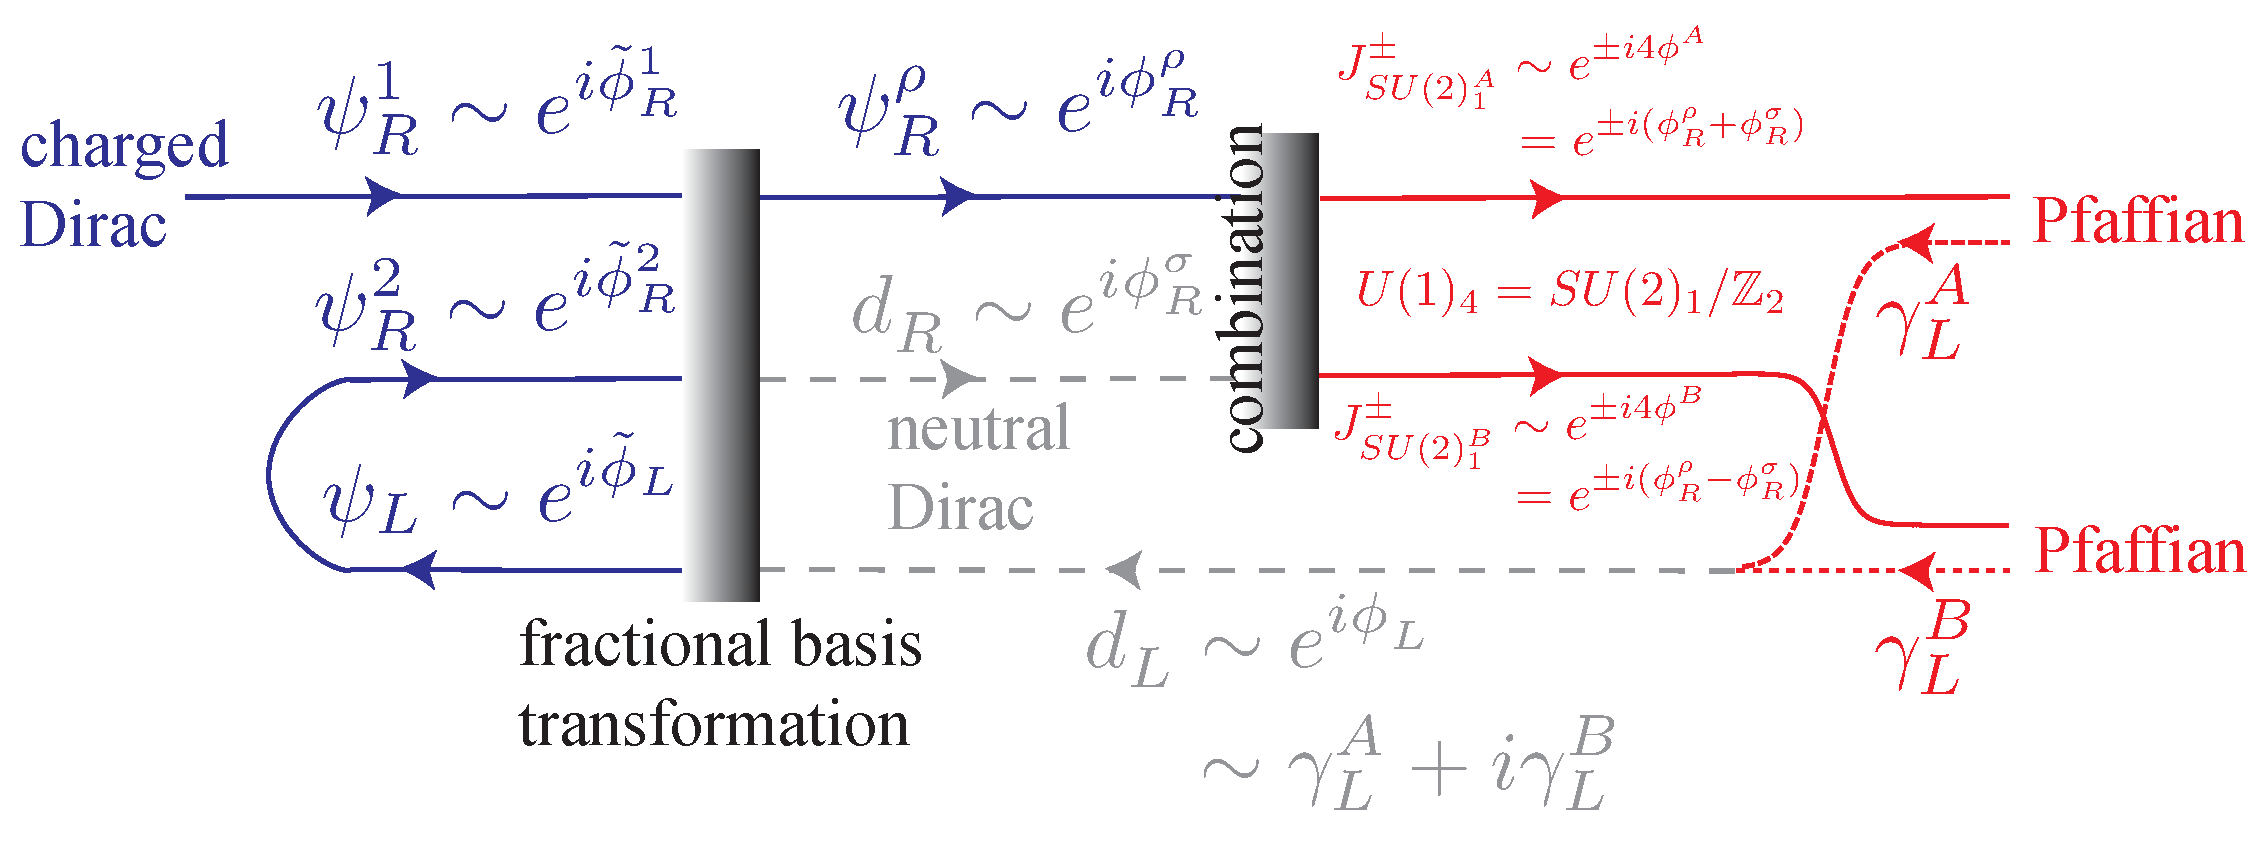
\includegraphics[width=1\textwidth]{fractionalization}
	\caption{Schematics of splitting a chiral Dirac channel into a pair of Pfaffian channels.}\label{fig:fractionalization}
\end{figure}

On the other hand, a chiral Dirac channel can be decomposed into a pair of chiral Pfaffian channels (see Fig.~\ref{fig:fractionalization} for a summary). First, perhaps from some channel re-construction, we append to the chiral Dirac channel an additional pair of counter-propagating Dirac modes. This can be realized by pulling a parabolic electronic/hole band from the conduction/valence band to the Fermi level, or introducing non-linear dispersion to the original chiral channel. In low-energy, the three Dirac fermion modes can be bosonized $\psi^{1,2}_R\sim e^{i\tilde\phi_R^{1,2}}$, $\psi_L\sim e^{-i\tilde\phi_L}$ and they are described by the multicomponent boson Lagrangian \begin{align}\widetilde{\mathcal{L}}_{\mathrm{Dirac}}=\frac{1}{2\pi}\partial_t\widetilde{\boldsymbol\phi}^T\tilde{K}\partial_x\widetilde{\boldsymbol\phi}+\partial_x\widetilde{\boldsymbol\phi}^T\tilde{V}\partial_x\widetilde{\boldsymbol\phi}\label{3Dirac}\end{align} for $\widetilde{\boldsymbol\phi}=(\tilde\phi_R^1,\tilde\phi_R^2,\tilde\phi_L)$, $\tilde{K}$ is the diagonal matrix $\tilde{K}=\mathrm{diag}(1,1,-1)$, and $\tilde{V}$ is some non-universal velocity matrix. A general composite excitation can be expressed by a vertex operator $e^{i{\bf m}\cdot\widetilde{\boldsymbol\phi}}$, for ${\bf m}$ an integral 3-vector, with spin $h_{\bf m}=|{\bf m}|^2/2$ and electric charge $q_{\bf m}={\bf m}^T\tilde{K}\tilde{\bf t}$ in units of $e$, where $\tilde{\bf t}=(1,1,1)$ is the charge vector.

Next we perform a {\em fractional} basis transformation \begin{align}\begin{array}{*{20}l}\phi^\rho_R=\tilde\phi^1_R+\tilde\phi^2_R+\tilde\phi_L \,, \\\phi^\sigma_R=\tilde\phi^1_R-\frac{1}{2}\tilde\phi^2_R+\frac{1}{2}\tilde\phi_L \,,\\\phi^\sigma_L=\tilde\phi^1_R+\frac{1}{2}\tilde\phi^2_R+\frac{3}{2}\tilde\phi_L \,.\end{array}\label{fracbasistrans0}\end{align} While the $\tilde{K}$ matrix is invariant under the transformation, the charge vector changes to $\tilde{\bf t}\to(1,0,0)$. $\psi^\rho_R\sim e^{i\phi^\rho_R}$ is the local electronic Dirac fermion that carries spin $1/2$ and electric charge $e$, and $d_{R/L}\sim e^{i\phi^\sigma_{R/L}}$ are counter-propagating electrically neutral Dirac fermions. As the $\tilde{K}$ matrix is still diagonal, these fermions have trivial mutual $2\pi$-monodromy and are local with respect to each other. However, it is important to notice that the neutral Dirac fermions $d_{R/L}$ actually consist of fractional electronic components.

Now we focus on the two $R$-moving Dirac channels. By pairing the Dirac fermions, they form two independent $SU(2)_1$ Kac-Moody current operators~\cite{bigyellowbook} \begin{align}J_3^{A/B}(z)&=i2\sqrt{2}\partial_z\phi^{A/B}_R(z)\label{SU2current} \,, \\J_\pm^{A/B}(z)&=\frac{J_1^{A/B}(z)\pm iJ_2^{A/B}(z)}{\sqrt{2}}=e^{\pm i4\phi^{A/B}_R(z)}\nonumber \,, \end{align} where $4\phi^A_R=\phi^\rho_R+\phi^\sigma_R$ and $4\phi^B_R=\phi^\rho_R-\phi^\sigma_R$. Both $SU(2)_1$ sectors are electrically charged so that the bosonic vertex operators $J_\pm^{A/B}$ carries charge $\pm e$. They obey the $SU(2)$ current algebra at level 1 \begin{align}J^\lambda_{\mathsf{i}}(z)J^{\lambda'}_{\mathsf{j}}(w)=\frac{\delta^{\lambda\lambda'}\delta_{\mathsf{ij}}}{(z-w)^2}+\sum_{\mathsf{k}=1}^3\frac{i\sqrt{2}\delta^{\lambda\lambda'}\varepsilon_{\mathsf{ijk}}}{z-w}J^\lambda_{\mathsf{k}}(w)+\ldots\label{SU2algebra}\end{align} for $\lambda,\lambda'=A,B$. It is crucial to remember that $J_\pm^A\sim\psi^\rho_Rd_R$ and $J_\pm^B\sim\psi^\rho_Rd_R^\dagger$ contains the fractional Dirac components $d_R$. Thus, the primitive local bosons are actually pairs of the current operators, i.e.~$e^{i8\phi^{A/B}_R}$. Equivalently, this renormalizes the compactification radius of the boson $4\phi^{A/B}_R$ so that in a closed periodic space-time geometry, we only require electronic Cooper pair combinations such as the charge $2e$ local operators \begin{gather}e^{i8\phi^A_R}=e^{i(4\tilde\phi^1_R+\tilde\phi^2_R+3\tilde\phi_L)}\sim(\psi^1_R)^4\psi^2_R(\psi_L^\dagger)^3\nonumber \,, \\e^{i8\phi^B_R}=e^{i(3\tilde\phi^2_R+\tilde\phi_L)}\sim(\psi^2_R)^3\psi_L^\dagger\end{gather} to be periodic. The incorporation of anti-periodic boundary condition for $J_\pm^{A/B}=e^{\pm i4\phi^{A/B}_R}$ results in the $\mathbb{Z}_2$-orbifold theory~\cite{Ginsparg88,DijkgraafVafaVerlindeVerlinde99} $U(1)_4=SU(2)_1/\mathbb{Z}_2$ for both $A$ and $B$ sectors. For instance, the primitive twist fields are given by $e^{\pm i\phi^{A/B}_R}$, which have $-1$ monodromy phase with $J_\pm^{A/B}$. 

At this point, including the $L$-moving neutral Dirac sector, we have recovered the muticomponent boson $\boldsymbol\phi=(\phi^A_R,\phi^B_R,\phi^\sigma_L)$ described by the Lagrangian \eqref{881}. Lastly, we simply have to decompose the remaining neutral Dirac into Majorana components, $d_L=(\gamma^A_L+i\gamma^B_L)/\sqrt{2}$. The $A$ and $B$ Pfaffian sectors can then be independently generated by the charged $U(1)_4$ boson $\phi^{A/B}_R$ and the neutral Majorana fermion $\gamma^{A/B}_L$. As a consistency check, the charge $e$ fermionic (normal ordered) combinations defined in \eqref{Pfaffianfields} \begin{align}\psi_4^A&\sim e^{i4\phi^A_R}\gamma_L^A\sim e^{i\tilde\phi^1_R}+e^{i(3\tilde\phi^1_R+\tilde\phi^2_R+3\tilde\phi_L)}\label{psi4def1} \,, \\\psi_4^B&\sim e^{i4\phi^B_R}\gamma_L^B\sim e^{i(-\tilde\phi^1_R+\tilde\phi^2_R-\tilde\phi_L)}-e^{i(\tilde\phi^1_R+2\tilde\phi^2_R+2\tilde\phi_L)}\nonumber\end{align} are in fact local quasi-electronic. %(The minus sign in the bosonized expression for $\psi_4^A$ comes from the Klein factors defined later in \eqref{ETcomm0} and \eqref{ETcomm1}).

Unlike in the gluing case where there is a gapping Hamiltonian \eqref{glueingH} that pastes a pair of Pfaffians into a Dirac, here in the splitting case we have simply performed some kind of fractional basis transformation that allows us to express Dirac as a pair of Pfaffians. In fact, one can check that the energy-momentum tensor of the Dirac theory \eqref{3Dirac} is identical to that of a pair of Pfaffians \eqref{Pfaffian}. However, this does not mean the Pfaffian primary fields are natural stable excitations. In fact, as long as there is a pair of co-propagating Pfaffian channels, all primary fields except the non-fractionalized electronic ones are unstable against the gluing Hamiltonian $\delta\mathcal{H}$ in \eqref{glueingH} and are generically gapped. In order for the Pfaffian \CFT to be stabilized, one has to suppress $\delta\mathcal{H}$. A possible way is to somehow spatially separate the pair. This issue is addressed in the subsection below using many-body interaction in the coupled wire model of a Dirac semimetal (or the \PHS Pfaffian \FQH state in Ref.~\cite{KaneSternHalperin17}).

%\subsubsection{\texorpdfstring{$AB$}{AB} symmetry}
%The bi-partition $\mathrm{Dirac}=\mathrm{Pfaffian}^A\otimes\mathrm{Pfaffian}^B$ carries a flip symmetry that exchanges the two Pfaffian sectors. When the two Pfaffian channels are spatially separated (see Fig.~\ref{fig:glueingsplitting}), the flip symmetry is simply the twofold rotation that exchanges the two parallel channels along their center-of-mass axis. We will use this flip operation to generate the $C_2$ symmetry in the interacting coupled wire model in the next subsection. Focusing on a single wire, the twofold symmetry flips \begin{align}C_2\phi^{A/B}_RC_2^{-1}=\phi^{B/A}_R+\frac{\pi}{8},\quad C_2\phi^\sigma_LC_2^{-1}=\phi^\sigma_L+\frac{\pi}{2}.\end{align} The constants phases ensures the $2\pi$ rotation $C_2^2$ associates the appropriate $-1$ twist phase 
%$e^{2\pi ih_X}$ determined by the spin $h_X$ of the primary field $X$. 


\subsection{Symmetry preserving massive interacting model}\label{sec:interactionmodels}

We begin with the 3D array of chiral Dirac strings in Fig.~\ref{fig:vortexlattice}. In Sec.~\ref{sec:DiracSemimetal}, we showed that the single-body coupled wire model \eqref{WeylTBHam} described a Dirac semimetal with two Weyl fermions (see Fig.~\ref{fig:Weylspectrum}). The system had emergent antiferromagnetic time reversal (AFTR) symmetries $\mathcal{T}_{11}$ and $\mathcal{T}_{\bar{1}1}$ along the diagonal and off-diagonal axes (see \eqref{WeylTBT11}). Together they generate an emergent lattice translation symmetry with a 2-wire unit cell, and separate the two Weyl points in the Brillouin zone. The symmetries are lowered beyond the effective model when the microscopic high-energy degrees of freedom are included. For example, the mass function \eqref{Jacobielliptic} that supports the Dirac vortex string lattice has a 4-wire periodic unit cell and only preserves one of the \AFTR symmetries $\mathcal{T}_{11}$ (see \eqref{massT11}). With the lowered translation symmetry, the two Weyl points now coincide at the same momentum. Inter-species (or inter-valley) mixing is forbidden by the remaining \AFTR symmetry and a (screw) twofold rotation symmetry $C_2$ about $z$ (see \eqref{WeylTBC2} and \eqref{massC2}). Previously in Sec.~\ref{sec:brokensymmetry}, we introduced symmetry breaking wire dimerizations in \eqref{DiracTBHam} that led to a massive Dirac insulator. In this section, we construct many-body gapping interactions that preserves the two \AFTR symmetries $\mathcal{T}_{11}$ and $\mathcal{T}_{\bar{1}1}$, the $C_2$ symmetry, as well as charge $U(1)$ conservation. 

\begin{figure}[htbp]
	\centering
	(a)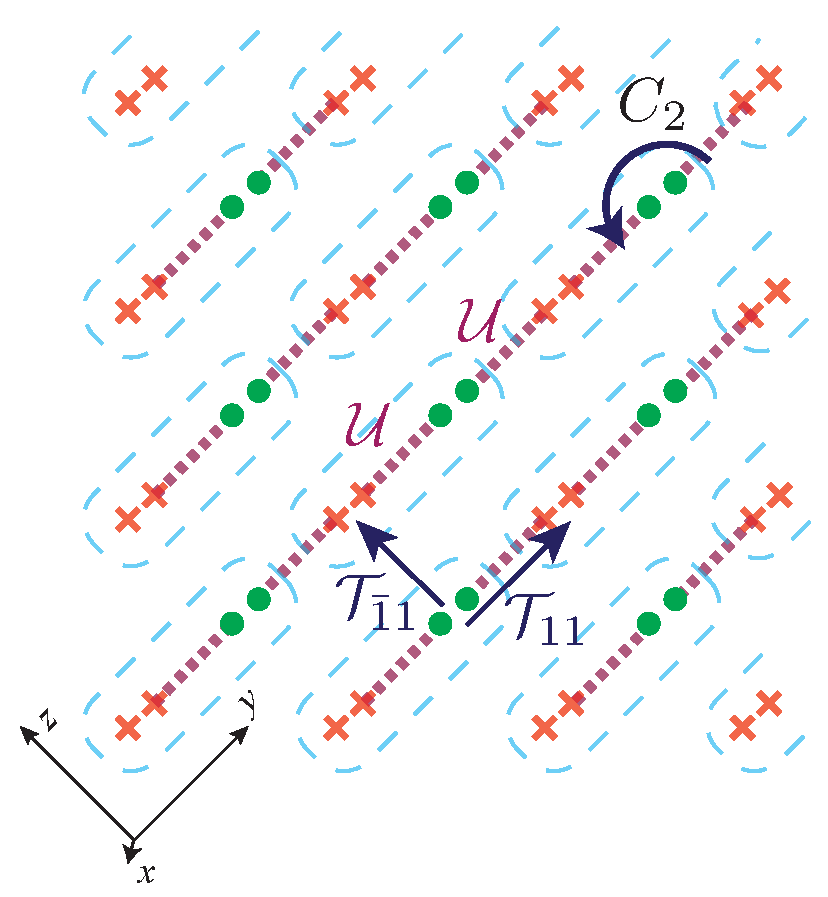
\includegraphics[width=0.5\textwidth]{gappinginteraction1}
	(b)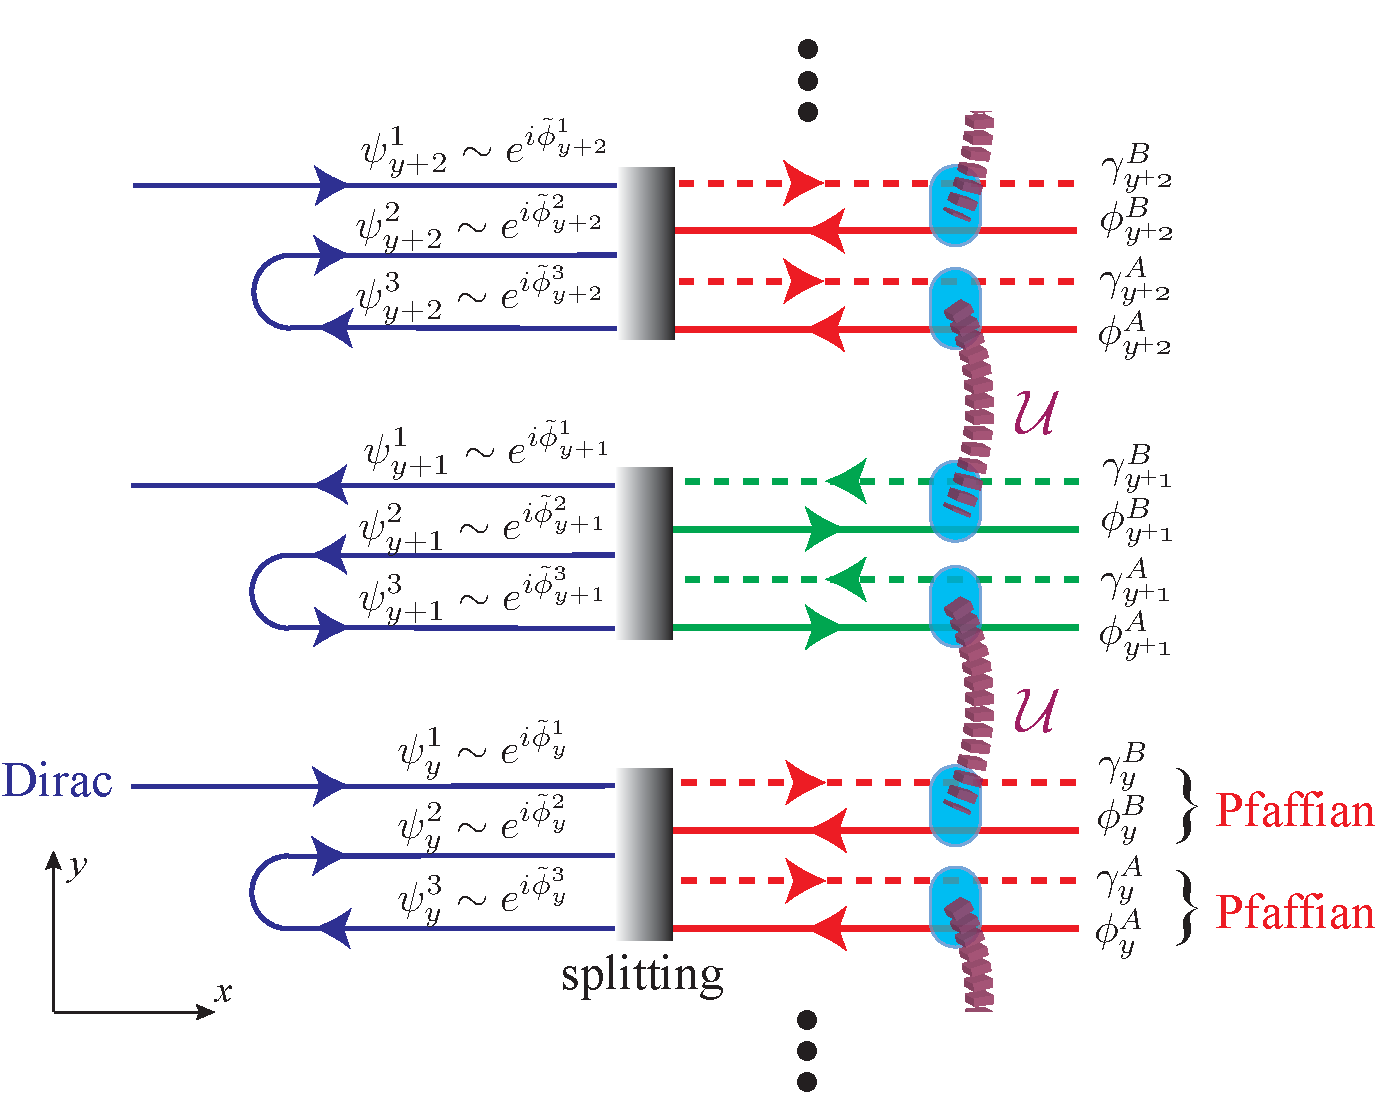
\includegraphics[width=0.9\textwidth]{gappinginteraction2}
	\caption[Symmetry preserving many-body gapping interaction.]{Symmetry preserving many-body gapping interaction. (a) Each {\color{red}$\boldsymbol\times$}/{\color{green}$\bullet$} represents a chiral Pfaffian channel into/out-of paper. Purple dashed line represents many-body gapping interaction $\mathcal{U}$ in \eqref{mbdint}. (b) Coupled wire model on a single layer along the diagonal axis.}\label{fig:gappinginteraction}
\end{figure}

The many-body gapping scheme is summarized in Fig.~\ref{fig:gappinginteraction}. From the previous subsection, we saw that each chiral Dirac channel can be decomposed into a pair of independent Pfaffian channels. They can then be backscattered in opposite directions to neighboring wires. Figure~\ref{fig:gappinginteraction}(a) shows a particular dimerization pattern of the Pfaffian channels that preserves the symmetries. In this case, the many-body backscattering interaction $\mathcal{U}$ is directed along the diagonal axis. In the limit when $\mathcal{U}$ is much stronger than the single-body electron tunneling in the previous semimetallic model \eqref{WeylTBHam}, the system decomposes into decoupled diagonal layers and it suffices to consider the interaction on a single layer. For convenience, we here change our spatial coordinates so that the diagonal axis is now labeled by $y$ and the wires now propagate along $x$.

Focusing on a single diagonal layer, the system in the non-interacting limit first consists of a 2D array of chiral Dirac strings with alternating propagating directions (see the left side of Fig.~\ref{fig:gappinginteraction}(b)). We notice that this is identical to the starting point of the coupled wire construction of the topological insulator Dirac surface state considered by Mross, Essin and Alicea in Ref.~\cite{MrossEssinAlicea15}. For instance, the alternating Dirac channels there were supported between magnetic strips with alternating orientations on the topological insulator surface, and an uniform nearest-channel electron tunneling recovered the massless 2D Dirac spectrum protected by the \AFTR symmetry. They then proceeded to propose symmetry preserving many-body gapping interactions facilitated by adding 2D \FQH strips between the channels. While this reconstruction trick can be applied on the 2D surface of a topological insulator, it is not feasible in our 3D situation and would require drastic modification of the bulk semimetal. Instead, here we propose an alternative gapping scheme that does not involve additional topological phases. In other words, we are going to construct a 3D gapped and layered topological phase solely from interacting electronic Dirac wires.

First, in order to implement the splitting described in the previous subsection, we assume each Dirac string consists of two Dirac channels going in one direction and a third Dirac channel going the opposite direction (see the left side of Fig.~\ref{fig:gappinginteraction}(b)). We denote the electronic Dirac fermions on the $y^{\mathrm{th}}$ wire by $\boldsymbol\psi_y=(\psi_y^1,\psi_y^2,\psi_y^3)$ and bosonize \begin{align}\psi_y^{1,2}(x)\sim e^{i\tilde\phi^{1,2}_y(x)},\quad\psi_y^3(x)\sim e^{-i\tilde\phi^3_y(x)}.\label{bosondef}\end{align} The sliding Luttinger liquid\cite{OHernLubenskyToner99,EmeryFradkinKivelsonLubensky00,VishwanathCarpentier01,SondhiYang01,MukhopadhyayKaneLubensky01} Lagrangian density is \begin{align}\mathcal{L}_{\mathrm{layer}}=\sum_{y=-\infty}^\infty\frac{(-1)^y\tilde{K}_{jk}}{2\pi}\partial_t\tilde\phi_y^j\partial_x\tilde\phi_y^k+\tilde{V}_{jk}\partial_x\tilde\phi_y^j\partial_x\tilde\phi_y^k \,, \label{Llayer}\end{align} where $\tilde{K}=(\tilde{K}_{jk})_{3\times3}=\mathrm{diag}(1,1,-1)$, $\tilde{V}$ is some non-universal velocity matrix, and repeating species indices $j,k$ are summed over. The boson operators obey the equal-time commutation relation (\hypertarget{ETCR}{ETCR}) \begin{align}&\left[\tilde\phi_y^j(x),\tilde\phi_{y'}^{j'}(x')\right]=c^{jj'}_{yy'}(x-x')\nonumber \,, \\=&i\pi(-1)^y\delta_{yy'}\tilde{K}^{jj'}\mathrm{sgn}(x'-x)\label{ETcomm0}\\&+i\pi(-1)^y\delta_{yy'}S^{jj'}\nonumber\\&+i\pi(-1)^{\mathrm{max}\{y,y'\}}\mathrm{sgn}(y-y')\Sigma^{jj'}\sigma_z^{y-y'+1}\nonumber\,, \end{align}
%\begin{align}\left[\tilde\phi_y^j(x),\tilde\phi_{y'}^{j'}(x')\right]=&i\pi(-1)^{\mathrm{max}\{y,y'\}}\Big[\delta_{yy'}\tilde{K}^{jj'}\mathrm{sgn}(x'-x)\nonumber\\&+\delta_{yy'}\mathrm{sgn}(j-j')+\mathrm{sgn}(y-y')\Big]\label{ETcomm0}\end{align} 
where $\mathrm{sgn}(s)=s/|s|=\pm1$ for $s\neq0$ and $\mathrm{sgn}(0)=0$, \begin{align}S=\left(\begin{smallmatrix}0&1&-1\\-1&0&1\\1&-1&0\end{smallmatrix}\right),\quad\Sigma=\left(\begin{smallmatrix}1&1&-1\\1&1&-1\\-1&-1&1\end{smallmatrix}\right),\label{Kleinfactors}\end{align} and $\sigma_z=\pm1$. The introduction of the specific Klein factors $S^{jj'}$, $\Sigma^{jj'}$ and the undetermined sign $\sigma_z$ are necessary for the correct representations of the $\mathcal{T}_{11}$ and $\mathcal{C}_2$ symmetries in the bosonization setting, and these choices will be justified below. The first line of \eqref{ETcomm0} is equivalent to the commutation relation between conjugate fields \begin{align}\left[\tilde\phi_y^j(x),\partial_{x'}\tilde\phi_{y'}^{j'}(x')\right]=2\pi i(-1)^y\delta_{yy'}\tilde{K}^{jj'}\delta(x-x') \,, \label{ETcomm00}\end{align} which is set by the ``$p\dot{q}$" term in $\mathcal{L}_{\mathrm{layer}}$. The alternating signs $(-1)^y$ in \eqref{ETcomm00} and \eqref{Llayer} changes the propagating directions from wire to wire. The second and third line of \eqref{ETcomm0} guarantee the correct anticommutation relations $\{e^{\pm i\tilde\phi^j_y},e^{\pm i\tilde\phi^{j'}_{y'}}\}=0$ between Dirac fermions along distinct channels $j\neq j'$ or distinct wires $y\neq y'$. The reason the $\tilde{C}_2$ matrix is defined in this form will become clear in the fractional basis discussed later in \eqref{bosonC2Pf}.

The anti-unitary \AFTR symmetry along the diagonal $\mathcal{T}_{11}$ direction transforms the bosons according to \begin{align}\mathcal{T}_{11}\tilde\phi^j_y\mathcal{T}_{11}^{-1}=-\tilde\phi^j_{y+1}+\frac{1+(-1)^y}{2}\tilde{K}^{jj}\pi.\label{bosonTR11}\end{align} The unitary $\mathcal{C}_2$ rotation takes \begin{gather}\mathcal{C}_2\tilde\phi^j_y\mathcal{C}_2^{-1}=\left(\tilde{C}_2\right)^j_{j'}\tilde\phi^{j'}_{-y}+(-1)^yv^j\frac{\pi}{2},\label{bosonC2}\\\tilde{C}_2=\left(\begin{smallmatrix}1&2&2\\2&1&2\\-2&-2&-3\end{smallmatrix}\right),\quad{\bf v}=\left(\begin{smallmatrix}v^1\\v^2\\v^3\end{smallmatrix}\right)=\left(\begin{smallmatrix}3\\-3\\1\end{smallmatrix}\right).\nonumber\end{gather} Moreover, we choose the representation so that the sign $\sigma_z$ in the \ETCR \eqref{ETcomm0} is preserved by the \AFTR operator but is flipped by the $C_2$ symmetry, \begin{align}\mathcal{T}_{11}\sigma_z\mathcal{T}_{11}^{-1}=\sigma_z,\quad\mathcal{C}_2\sigma_z\mathcal{C}_2^{-1}=-\sigma_z.\end{align} 

The \ETCR \eqref{ETcomm0} is consistent with the \AFTR symmetry. This means that evaluating $\mathcal{T}_{11}\left[\tilde\phi_y^j(x),\tilde\phi_{y'}^{j'}(x')\right]\mathcal{T}_{11}^{-1}$ by taking the \AFTR operator inside the commutator \begin{align}&\left[\mathcal{T}_{11}\tilde\phi_y^j(x)\mathcal{T}_{11}^{-1},\mathcal{T}_{11}\tilde\phi_{y'}^{j'}(x')\mathcal{T}_{11}^{-1}\right]\nonumber\\&=\left[\tilde\phi_{y+1}^j(x),\tilde\phi_{y'+1}^{j'}(x')\right]=c^{jj'}_{y+1,y'+1}(x-x')\end{align} yields the same outcome as taking the \TR of the purely imaginary scalar \begin{align}\mathcal{T}_{11}c^{jj'}_{yy'}(x-x')\mathcal{T}_{11}^{-1}=-c^{jj'}_{yy'}(x-x').\end{align} The \ETCR \eqref{ETcomm0} is also consistent with the $\mathcal{C}_2$ symmetry \begin{align}(\tilde{C}_2)^{j_1}_{j'_1}c^{j'_1j'_2}_{-y_1,-y_2}(x_1-x_2)(\tilde{C}_2)^{j_2}_{j'_2}=\mathcal{C}_2c^{j_1j_2}_{y_1y_2}(x_1-x_2)\mathcal{C}_2^{-1}.\label{ETcommC2consistent}\end{align} This is because the Klein factors \eqref{Kleinfactors} are $C_2$ symmetric \begin{align}\tilde{C}_2S\tilde{C}_2^T=S,\quad\tilde{C}_2\Sigma\tilde{C}_2^T=\Sigma.\end{align} Notice that the undetermined sign $\sigma_z$, which is odd under $\mathcal{C}_2$, in \eqref{ETcomm0} is essential for the \ETCR to be consistent with $C_2$.

The last term in the \AFTR operation \eqref{bosonTR11} makes sure \begin{align}\mathcal{T}_{11}^2\tilde\phi_y^j(x)\mathcal{T}_{11}^{-2}=\tilde\phi_{y+2}^j+(-1)^y\tilde{K}^{jj}\pi,\end{align} which is necessary for $\mathcal{T}^2_{11}=(-1)^F\mathrm{translation}(2{\bf e}_y)$. Here the fermion parity operator is $(-1)^F=e^{i\pi\sum_{yj}N_y^j}$, where \begin{align}N_y^j=\int\frac{dx}{2\pi}\partial_x\tilde\phi_y^j(x)\label{numop}\end{align} is the number operator. The vector ${\bf v}$ in the $\mathcal{C}_2$ operation \eqref{bosonC2} satisfies $(\delta^j_{j'}+(\tilde{C}_2)^j_{j'})v^{j'}/2=\tilde{K}^{jj}$, and consequently \begin{align}\mathcal{C}_{2}^2\tilde\phi_y^j(x)\mathcal{C}_{2}^{-2}=\tilde\phi_y^j+(-1)^y\tilde{K}^{jj}\pi,\end{align} which is consistent with $\mathcal{C}_2^2=(-1)^F$. Lastly, it is straightforward to check that the symmetry representations \eqref{bosonTR11} and \eqref{bosonC2} are compatible with the algebraic relation \eqref{C2Trelation}, i.e. \begin{align}&\mathcal{C}_2\mathcal{T}_{11}\tilde\phi^j_y\mathcal{T}_{11}^{-1}\mathcal{C}_2^{-1}\\&=(-1)^F\mathcal{T}_{11}^{-1}\mathcal{C}_2\tilde\phi^j_y\mathcal{C}_2^{-1}\mathcal{T}_{11}(-1)^{-F}.\nonumber\end{align}

%The, at first sight, obscured expression of the $3\times3$ rotation matrix $C_2$ in \eqref{bosonC2} actually takes a much simply form under the fractional basis transformation considered in the previous subsection~\ref{sec:gluing}. We defer this simplification a bit later, but at this point, we notice that the Klein fators $S$ and $\Sigma$ in the \ETCR \eqref{ETcomm0} are chosen to be consistent with the $C_2$ symmetry, \begin{align}C_2SC_2^T=S,\quad C_2\Sigma C_2^T=\Sigma.\end{align} 

Following the splitting scheme summarized in Fig.~\ref{fig:fractionalization}, we again define a fractional basis transformation (c.f.~\eqref{fracbasistrans0}) \begin{align}\begin{pmatrix}\phi^\rho_y\\\phi^{\sigma1}_y\\\phi^{\sigma2}_y\end{pmatrix}=\left(\begin{array}{*{20}c}1&1&1\\1&-1/2&1/2\\1&1/2&3/2\end{array}\right)\left(\begin{array}{*{20}c}\tilde\phi^1_y\\\tilde\phi^2_y\\\tilde\phi^3_y\end{array}\right)\label{fracbasistrans}\end{align} for each wire, so that $\psi^\rho_y\sim e^{i\phi^\rho_y}$ is a Dirac fermion carrying electric charge $e$, $d^{\sigma1}_y\sim e^{i\phi^{\sigma1}_y}$ ($d^{\sigma2}_y\sim e^{i\phi^{\sigma2}_y}$) is an electrically neutral Dirac fermion propagating in the same (resp.~opposite) direction as $\psi^\rho_y$.

For convenience, sometimes we combine the transformed bosonized variables into $\boldsymbol\phi_y=(\phi^1_y,\phi^2_y,\phi^3_y)=(\phi^A_y,\phi^B_y,\phi^{\sigma2}_y)$, which is related to the original local ones in \eqref{Llayer} by $\phi^J_y=G^J_j\tilde\phi^j_y$ where \begin{align}G=\begin{pmatrix}1/2&1/8&3/8\\0&3/8&1/8\\1&1/2&3/2\end{pmatrix}.\end{align} The \AFTR symmetry operation \eqref{bosonTR11} becomes \begin{align}\mathcal{T}_{11}\phi^I_y\mathcal{T}_{11}^{-1}=-\phi^I_{y+1}+\frac{1+(-1)^y}{2}\pi\kappa^I\label{bosonTR11Pf}
%\mathcal{T}_{11}\phi^{A/B}_y\mathcal{T}_{11}^{-1}&=-\phi^{A/B}_{y+1}+\frac{1+(-1)^y}{2}\pi,\nonumber\\\mathcal{T}_{11}\phi^{\sigma 2}_y\mathcal{T}_{11}^{-1}&=-\phi^{\sigma 2}_{y+1}.
\end{align} where $\kappa^I=G^I_j\tilde{K}^{jj}$ which is $1/4$ for $I=1,2$ and $0$ for $I=3$. The $C_2$ transformation \eqref{bosonC2} becomes \begin{gather}\mathcal{C}_2\phi^I_y\mathcal{C}_2^{-1}=\left(C_2\right)^I_J\phi^J_{-y}+(-1)^yG^I_jv^j\frac{\pi}{2},\label{bosonC2Pf}\\C_2=G\tilde{C}_2G^{-1}=\left(\begin{smallmatrix}0&1&0\\1&0&0\\0&0&-1\end{smallmatrix}\right),\quad G{\bf v}=\left(\begin{smallmatrix}3/2\\-1\\3\end{smallmatrix}\right).\nonumber\end{gather} The $3\times3$ $C_2$ matrix takes a much simpler form here using the fractional basis than in \eqref{bosonC2}. In fact, the original $\tilde{C}_2$ matrix in the local basis in \eqref{bosonC2} was defined so that $C_2=G\tilde{C}_2G^{-1}$ would act according to \eqref{bosonC2Pf}. Roughly speaking, ignoring the constant phases $G{\bf v}$, the $C_2$ symmetry switches $\phi^A_y\leftrightarrow\phi^B_{-y}$ and sends $\phi^{\sigma2}_y\to-\phi^{\sigma2}_{-y}$.

Next, we combine these co-propagating pair of fermions to form two $SU(2)_1$ current algebras (c.f.~\eqref{SU2current} and \eqref{SU2algebra}) \begin{align}&J_3^{A/B}(y,w)=i2\sqrt{2}\partial_w\phi^{A/B}_y(w)\nonumber \,, \\&J_\pm^{A/B}(y,w)=e^{\pm i4\phi^{A/B}_y(w)} \,, %\\&4\phi^A_y(w)=\phi^\rho_y(w)+\phi^{\sigma1}_y(w),\quad 4\phi^B_y(w)=\phi^\rho_y(w)-\phi^{\sigma1}_y(w)\nonumber
\end{align} where $w\sim\tau+(-1)^yx$ is the complex spacetime parameter. As a reminder, the charge $\pm e$ bosons $J^{A/B}_\pm$ are non-electronic fractional operators, although they carry non-fractional statistics.

The remaining counter-propagating neutral Dirac fermion can be decomposed into real and imaginary components \begin{align}d_y^{\sigma}(w)\sim\cos\phi^{\sigma2}_y(w)+i\sin\phi^{\sigma2}_y(w).\end{align} Majorana fermions can be constructed by multiplying these components with ``Jordan-Wigner" string \begin{align}\gamma^A_y&\sim\cos\phi^{\sigma2}_y\prod_{y'>y}(-1)^{N_{y'}^2+N_{y'}^3},\nonumber\\\gamma^B_y&\sim\sin\phi^{\sigma2}_y\prod_{y'>y}(-1)^{N_{y'}^2+N_{y'}^3},\label{MFdef}\end{align} where $N^j_y$ are the number operators defined in \eqref{numop}, so that they obey mutual fermionic statistics $\{\gamma^\lambda_y(x),\gamma^{\lambda'}_{y'}(x')\}=\delta^{\lambda\lambda'}\delta_{yy'}\delta(x-x')$, for $\lambda,\lambda'=A,B$. Similar to the charge  $\pm e$ bosons $J^{A/B}_\pm$, the electrically neutral Dirac fermion $d_y^\sigma$ and consequently the Majorana fermions $\gamma^{A/B}_y$ are also non-electronic fractional operators. This $AB$-decomposition splits each Dirac wire into a pair of decoupled Pfaffian sectors (see Fig.~\ref{fig:gappinginteraction}(b)).

Before we move on to the symmetric interaction, some further elaborations are needed for the number operators $N_y^j$ and their corresponding fermion parity operators $e^{i\pi N_y^j}$. In our construction, the counter-propagating pair of channels with $j=2,3$ are appended to the original one with $j=1$ to make the Pfaffian fractionalization feasible. We choose the Hilbert space so that the two additional fermion parity operators agree, $e^{i\pi N_y^2}=e^{i\pi N_y^3}$. However, we allow fluctuations to the combined parity $e^{i\pi(N_y^2+N_y^3)}$ and only require it squares to the identity, $e^{2\pi i(N_y^2+N_y^3)}=1$. In other words, $e^{i\pi(N_y^2+N_y^3)}=e^{-i\pi(N_y^2+N_y^3)}$ and it does not matter which one we take as $(-1)^{N_y^2+N_y^3}$ in the ``Jordan-Wigner" string in \eqref{MFdef}. This convention will also be useful later in seeing that the many-body interaction is exactly solvable and symmetry preserving. Extra care is sometimes required. For example, unlike the original Dirac channel where the parity is simply $(-1)^{N_y^1}=e^{\pm i\pi N_y^1}$ because $e^{2\pi iN_y^1}=1$, the individual parity operators $(-1)^{N_y^{2,3}}$ of these additional channels are not well-defined because $e^{2\pi iN_y^{2,3}}\neq1$, i.e.~$e^{i\pi N_y^{2,3}}\neq e^{-i\pi N_y^{2,3}}$. Also, although $e^{2\pi i(N_y^2+N_y^3)}=1$, one cannot in general modify a boson angle parameter simply by $\Theta\to\Theta+2\pi i(N_y^2+N_y^3)$ because $\Theta$ and the number operators may not commute. For instance, using the Baker-Campbell-Hausdorff formula and the \ETCR \eqref{ETcomm0}, $e^{i4\phi^{A/B}}$ and $e^{i4\phi^{A/B}+2\pi i(N_y^2+N_y^3)}$ are off by a minus sign.

The Pfaffian fractionalization is stabilized by the inter-wire many-body backscattering interaction (see Fig.~\ref{fig:gappinginteraction}(b)) \begin{align}\mathcal{U}&=-u\sum_{y=-\infty}^\infty\cos\phi^{\sigma2}_{y+1}\sin\phi^{\sigma2}_y\cos\left(4\phi^A_{y+1}-4\phi^B_y\right)\nonumber \,,\\
&=-u\sum_{y=-\infty}^\infty(-1)^yi\gamma^A_{y+1}\gamma^B_y\cos\left(\Theta_{y+1/2}\right),\label{mbdint}\end{align} for $\Theta_{y+1/2}(x)=4\phi^A_{y+1}(x)-4\phi^B_y(x)+\pi(N_{y+1}^2+N_{y+1}^3)$. Previously in \eqref{psi4def1}, we saw that the combinations $\psi_4^A\sim e^{i4\phi^A}\gamma^A$ and $\psi_4^B\sim e^{i4\phi^B}\gamma^B$ can be decomposed into products of electron operators. Similarly, each interaction in the first line of \eqref{mbdint} can be decomposed into products in the form of $e^{\pm i(\phi^{\sigma2}_{y+1}\pm4\phi^A_{y+1})}e^{\pm i(\phi^{\sigma2}_y\pm4\phi^B_y)}$ (with some scalar $U(1)$ coefficient), where the exponents $\phi^{\sigma2}\pm4\phi^{A/B}$ are linear integral combinations of $\tilde\phi^j$. Thus, the interaction can be re-written in terms of backscatterings of local electronic operators. However, we will omit the electronic expression as \eqref{mbdint} is more useful in discussing ground state and symmetries. 

$\mathcal{U}$ describes a symmetry-preserving exactly solvable model. Using the \ETCR \eqref{ETcomm0} it is straightforward to check that the (normal ordered) order parameters \begin{align}\mathcal{O}_{y+1/2}^F(x)=i\gamma^A_{y+1}(x)\gamma^B_y(x),\quad\mathcal{O}_{y+1/2}^\Theta(x)=e^{i\Theta_{y+1/2}(x)}\label{orderparameters}\end{align} mutually commute, i.e. $\left[\mathcal{O}_{y+1/2}^{F/\Theta}(x),\mathcal{O}_{y'+1/2}^{F/\Theta}(x')\right]=0$. Therefore, the model is exactly solvable, and its ground states are characterized by the ground state expectation values (\hypertarget{GEV}{GEV}) of the order parameters \begin{align}l_0\langle\mathcal{O}_{y+1/2}^F\rangle=(-1)^y\langle\mathcal{O}_{y+1/2}^\Theta\rangle=\pm1 \,, \end{align} so that the interacting energy $\langle\mathcal{U}\rangle$ is minimized, where $l_0$ is some non-universal microscopic length scale. Pinning the \GEV $\langle\Theta_{y+1/2}\rangle=n_{y+1/2}\pi$, for $n_{y+1/2}\in\mathbb{Z}$, gaps all degrees of freedom in the charged $U(1)_4^{A/B}=SU(2)_1^{A/B}$ sector. The remaining neutral fermions are gapped by the decoupled Majorana backscattering \begin{align}\delta\mathcal{H}_{\mathrm{Majorana}}=u\sum_{y=-\infty}^\infty(-1)^yi\langle\mathcal{O}^\Theta_{y+1/2}\rangle\gamma^A_{y+1}\gamma^B_y.\label{MajHam}\end{align} It is worth noting that a $\pi$-kink excitation of $\langle\Theta_{y+1/2}\rangle$ flips the Majorana mass in \eqref{MajHam} and therefore bounds a zero energy Majorana bound state~\cite{Kitaevchain}. A $\pi$-kink at $x_0$ can be created by the vertex operators $e^{\pm i\phi^A_{y+1}(x_0)}$ or $e^{\pm i\phi^B_y(x_0)}$ which carry $\pm1/4$ of an electric charge. (Recall the bosonic vertices $e^{i4\phi^{A/B}_y}$ carry charge $e$.) This $e/4$ excitation therefore corresponds to the Ising anyon in the Pfaffian \FQH state.

From the \AFTR symmetry action \eqref{bosonTR11Pf}, one can show that the Majorana fermions \eqref{MFdef} transform according to \begin{align}\mathcal{T}_{11}\gamma^A_y\mathcal{T}_{11}^{-1}=\gamma^A_{y+1},\quad\mathcal{T}_{11}\gamma^B_y\mathcal{T}_{11}^{-1}=-\gamma^B_{y+1}.\end{align} Therefore the fermion order parameter $\mathcal{O}^F_{y+1/2}=i\gamma^A_{y+1}\gamma^B_y$ \eqref{orderparameters} is translated under the antiunitary symmetry \begin{align}\mathcal{T}_{11}\mathcal{O}^F_{y+1/2}\mathcal{T}_{11}^{-1}=\mathcal{O}^F_{y+3/2}.\label{T11OF}\end{align} The boson angle parameter $\Theta_{y+1/2}$ defined below \eqref{mbdint} changes to $-\Theta_{y+3/2}-(-1)^y\pi$ under \AFTR, and therefore the boson order parameter $\mathcal{O}^\Theta_{y+1/2}=e^{i\Theta_{y+1/2}}$ is flipped and translated \begin{align}\mathcal{T}_{11}\mathcal{O}^\Theta_{y+1/2}\mathcal{T}_{11}^{-1}=-\mathcal{O}^\Theta_{y+3/2}.\label{T11OT}\end{align} Together, \eqref{T11OF} and \eqref{T11OT} show that the many-body interaction $\mathcal{U}$ in \eqref{mbdint} is \AFTR symmetric.

The $C_2$ action \eqref{bosonC2} flips the number operator $\mathcal{C}_2(N_y^2+N_y^3)\mathcal{C}_2^{-1}=-N_{-y}^2-N_{-y}^3$, and therefore the parity operators appear in the ``Jordan-Wigner" string \eqref{MFdef} are $C_2$ symmetric, $\mathcal{C}_2(-1)^{N_y^2+N_y^3}\mathcal{C}_2^{-1}=(-1)^{N_{-y}^2+N_{-y}^3}$. With the help of the $C_2$ action \eqref{bosonC2Pf} in the fractional basis, one sees that $\mathcal{C}_2\cos\phi^\sigma_y\mathcal{C}_2^{-1}=(-1)^{y+1}\sin\phi^\sigma_{-y}$ and $\mathcal{C}_2\sin\phi^\sigma_y\mathcal{C}_2^{-1}=(-1)^{y+1}\cos\phi^\sigma_{-y}$ and thus the Majorana fermions \eqref{MFdef} transform according to \begin{align}\mathcal{C}_2\gamma^A_y\mathcal{C}_2^{-1}=(-1)^{y+1}\gamma^B_{-y}(-1)^{F_{2+3}},\\\mathcal{C}_2\gamma^B_y\mathcal{C}_2^{-1}=(-1)^{y+1}\gamma^A_{-y}(-1)^{F_{2+3}},\nonumber\end{align} where $(-1)^{F_{2+3}}=\prod_{y=-\infty}^\infty(-1)^{N_y^2+N_y^3}$ is the total fermion parity of channel 2 and 3. This shows the fermion order parameter is odd under $C_2$ \begin{align}&\mathcal{C}_2\mathcal{O}^F_{y+1/2}\mathcal{C}_2^{-1}\nonumber\\&=i(-1)^{y+2}\gamma^B_{-y-1}(-1)^{F_{2+3}}(-1)^{y+1}\gamma^A_{-y}(-1)^{F_{2+3}}\nonumber\\&=-i\gamma^A_{-y}\gamma^B_{-y-1}=-\mathcal{O}^F_{-y-1/2}.\label{C2OF}\end{align} On the other hand, one can also show from the $C_2$ action \eqref{bosonC2Pf} that the boson angle parameter changes as $\mathcal{C}_2\Theta_{y+1/2}\mathcal{C}_2^{-1}=-\Theta_{-y-1/2}-(-1)^y\pi$ and therefore the boson order parameter $\mathcal{O}^\Theta_{y+1/2}=e^{i\Theta_{y+1/2}}$ is conjugated and flipped under $C_2$ \begin{align}\mathcal{C}_2\mathcal{O}^\Theta_{y+1/2}\mathcal{C}_2^{-1}=-{\mathcal{O}^\Theta_{-y-1/2}}^\dagger.\label{C2OT}\end{align} When combined together, the minus signs in \eqref{C2OF} and \eqref{C2OT} cancel and they show that the many-body interaction $\mathcal{U}$ in \eqref{mbdint} preserves $C_2$.

Now that we have introduced symmetry preserving gapping interactions on a single diagonal layer, we can extend it to the entire 3D structure by transferring \eqref{mbdint} to all layers using the off-diagonal \AFTR operator $\mathcal{T}_{\bar{1}1}$ (see Fig.~\ref{fig:gappinginteraction}(a)). The resulting state belongs to a topological phase in three dimensions with an excitation energy gap. It preserves both \AFTR symmetries $\mathcal{T}_{11}$ and $\mathcal{T}_{\bar{1}1}$ as well as the (screw) $C_2$ symmetry. The choice of writing this dissertation with a specific model with these symmetries was intentional, we wanted to work out the simplest example with specific symmetries explicitly for illustrative reasons instead of doing a more general classification type argument. We leave the SPT-SET correspondences for general symmetries as an open question, but we expect that the methods presented in this work can be useful in exploring them.


\subsection{Antiferromagnetic stabilization}\label{sec:AFMstabilization}
The exactly-solvable many-body interacting model \eqref{mbdint} (see also Fig.~\ref{fig:gappinginteraction}) shows that the Dirac semimetal \eqref{WeylTBHam} can acquire a many-body mass gap without breaking symmetries. However, it is not clear how dominant or stable the topological phase described by \eqref{mbdint} is. There are alternative interactions that lead to other metallic or insulating phases that preserve or break symmetries. The scaling dimensions and the relevance of the interaction terms~\cite{Fradkinbook,Tsvelikbook} can be tuned by the velocity matrix $V_{jk}$ in \eqref{Llayer} that is affected by forward scattering interactions among co-propagating channels. Instead of considering energetics, we focus on a topological deliberation -- inspired by the coupled wire construction of quantum Hall states~\cite{KaneMukhopadhyayLubensky02,TeoKaneCouplewires} -- that can drastically reduce the number of possible interactions and may stabilize the desired interactions when applied to materials.

The coupled wire model considered so far assumes all electronic Dirac modes at the Fermi level have zero momentum $k_x=0$. This is convenient for the purpose of constructing an exactly solvable model because momentum is automatically conserved by the backscattering interactions. However, this also allows a huge collection of competing interactions. We propose the application of a commensurate modulation of magnetic field to restrict interactions that conserve momentum. There are multiple variations to the application, which depend on the details of the Dirac material and the Dirac vortices. To illustrate the idea, we present one possible simple scenario.

\begin{figure}[htbp]
	\centering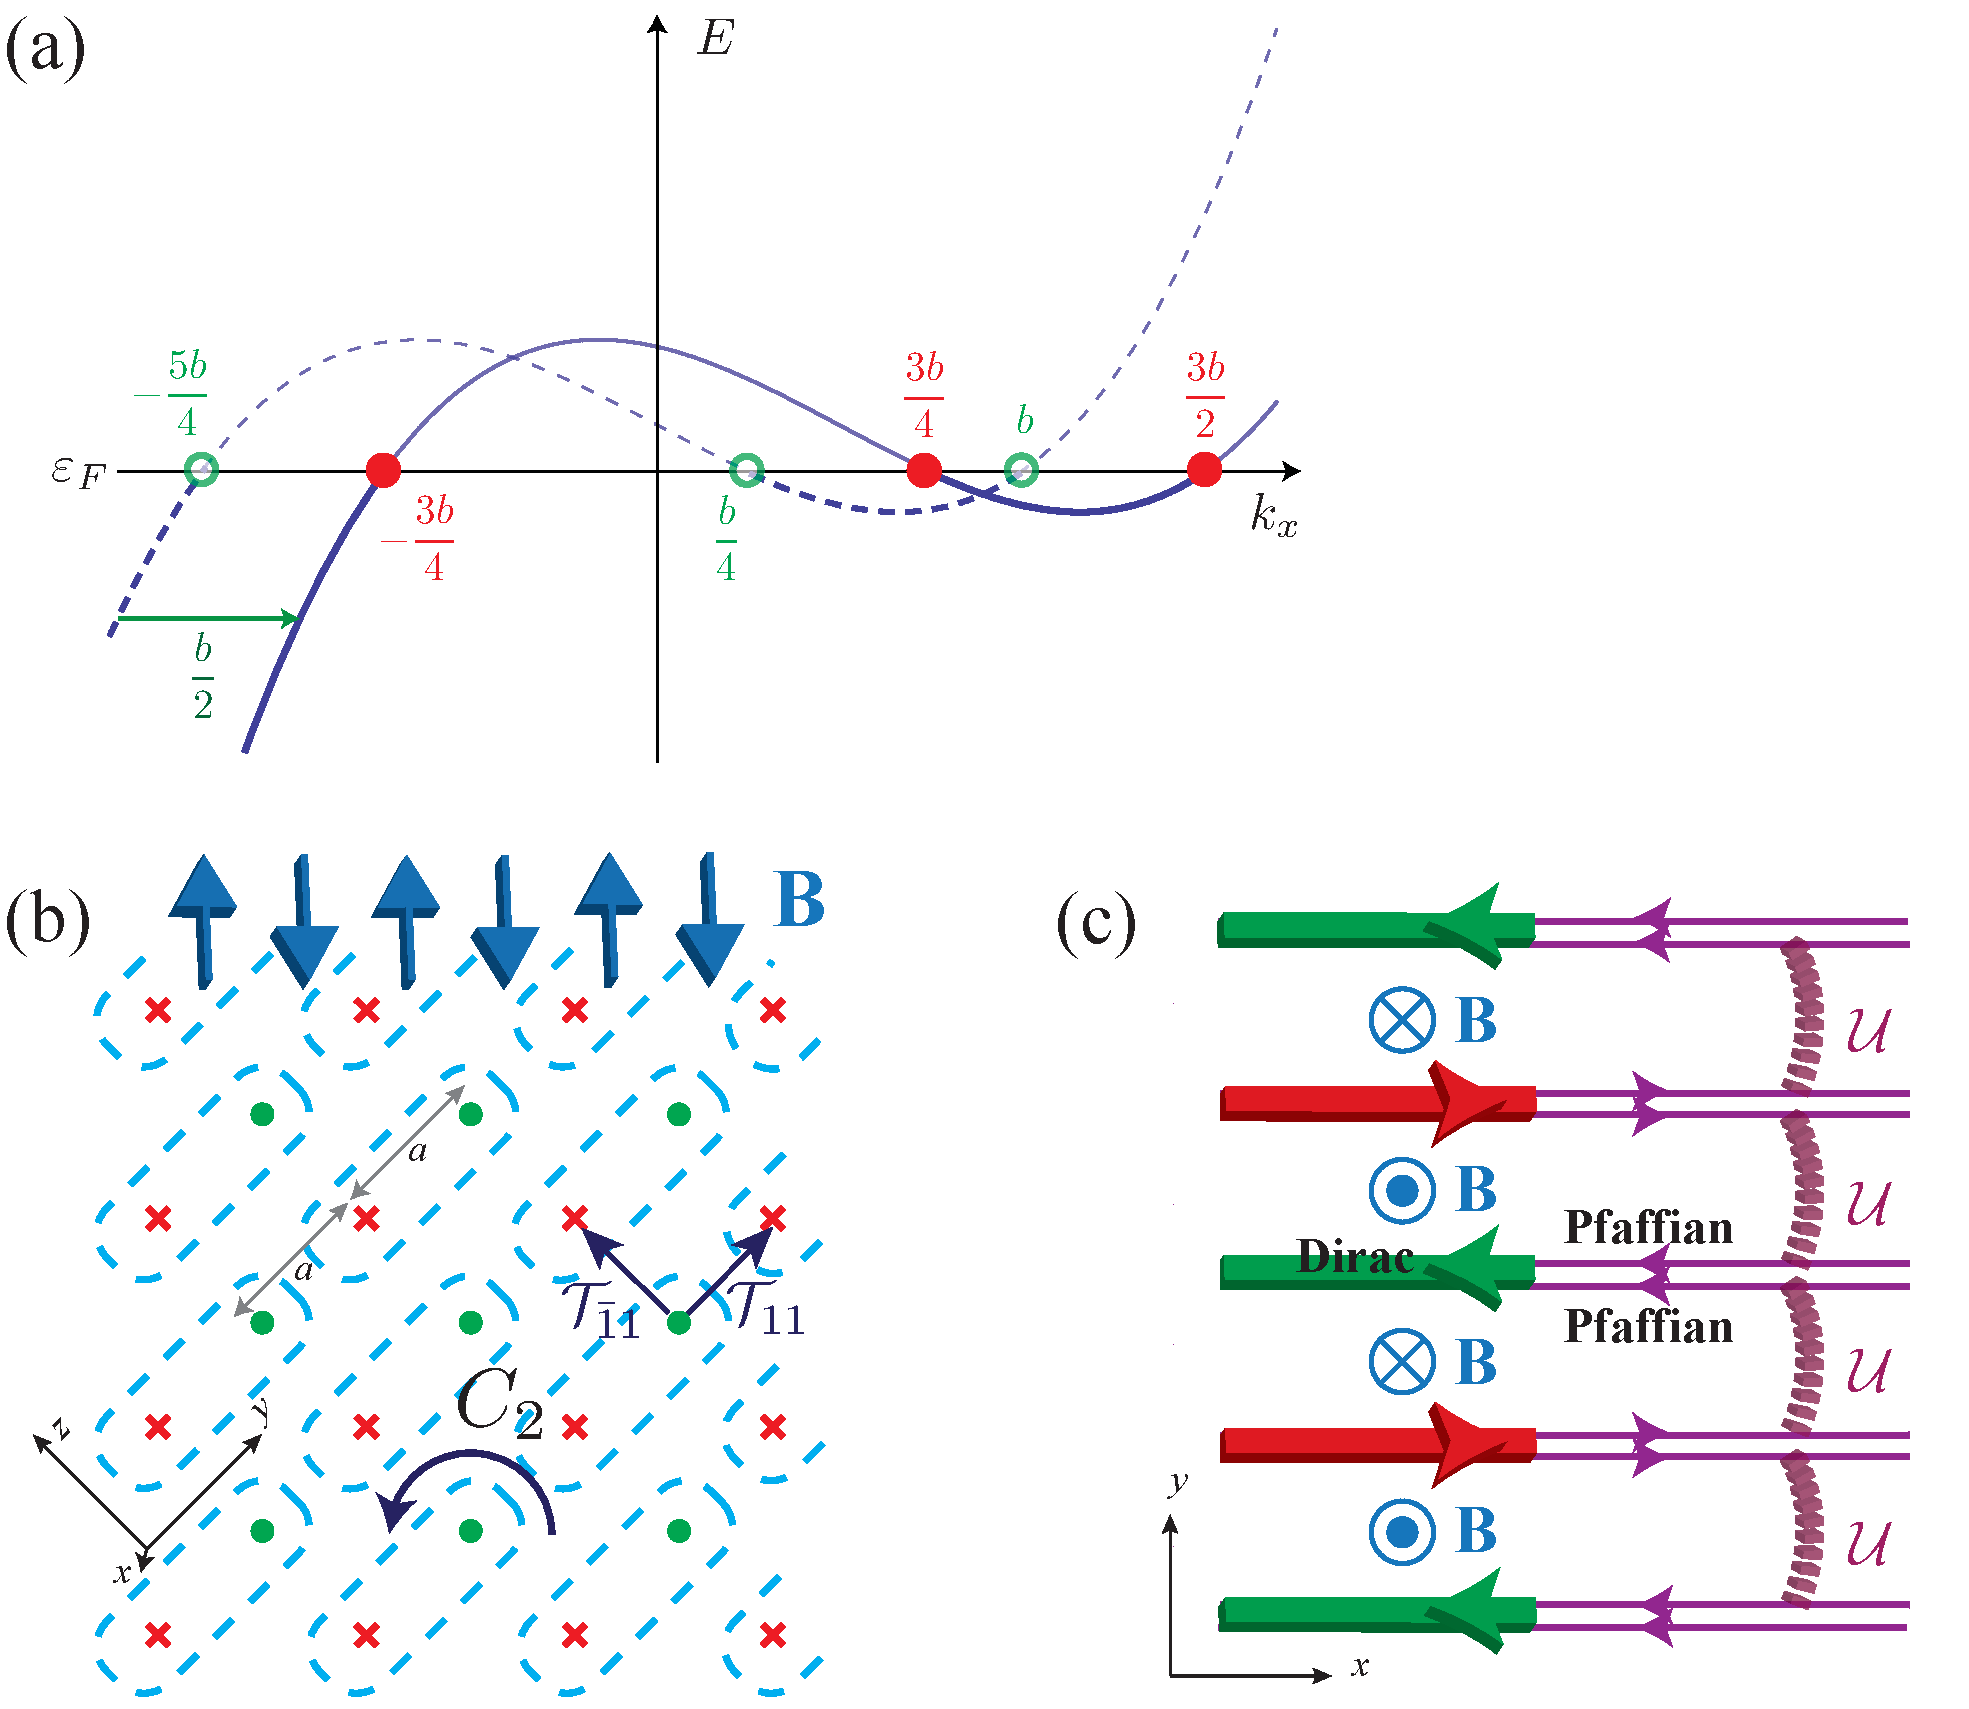
\includegraphics[width=0.9\textwidth]{afm}
	\caption[Antiferromagnetic stabilization.]{(a) The energy dispersion $E_{y=2l}(k_x)$ with (solid curve) or without (dashed curve) the alternating magnetic field. (b) The alternating magnetic field configuration that preserves the AFTR and $C_2$ symmetries. (c) The alternating magnetic field across a single layer along the $xy$ plane.}\label{fig:afm}
\end{figure}

First we go back to a single Dirac wire and consider a non-linear dispersion \begin{align}E^0_{y=2l}(k_x)&=\frac{\hbar v}{b^2}(k_x-k_F^1)(k_x-k_F^2)(k_x-k_F^3),\nonumber\\E^0_{y=2l+1}(k_x)&=-\frac{\hbar v}{b^2}(k_x+k_F^1)(k_x+k_F^2)(k_x+k_F^3),\end{align} where $v$ and $b$ are some non-universal velocity and wave number parameters. We assume $k_F^2<k_F^3<k_F^1$ so that when the Fermi energy is at $\varepsilon_F=0$, there are two right (left) moving modes at $k_x=k_F^1,k_F^2$ and one left (resp.~right) moving one at $k_X=k_F^3$ along an even (resp.~odd) wire. This matches the three-channel Dirac wire \eqref{3Dirac} used in the splitting scheme in Sec.~\ref{sec:gluing}. We assume the three Fermi wave numbers satisfy a commensurate condition \begin{align}2k_F^1+k_F^2-3k_F^3=0,\label{kcomm}\end{align} and we set \begin{align}b=2(k_F^3-k_F^1-k_F^2).\label{bcomm1}\end{align} The dashed band in Fig.~\ref{fig:afm}(a) shows one commensurate energy dispersion along an even wire.

Next, we consider a spatially modulating magnetic field ${\bf B}({\bf r})=B({\bf r}){\bf e}_{11}$, where \begin{align}B({\bf r})=\sum_{m=-\infty}^\infty B_m\sin\left[\pi\frac{\sqrt{2}(2m+1)}{a}{\bf e}_{\bar{1}1}\cdot{\bf r}\right],\end{align} ${\bf e}_{11}=({\bf e}_y+{\bf e}_z)/\sqrt{2}$ and ${\bf e}_{\bar{1}1}=(-{\bf e}_y+{\bf e}_z)/\sqrt{2}$, that preserves both the \AFTR and $C_2$ symmetries, \begin{align}B({\bf r}+a{\bf e}_y)=B({\bf r}+a{\bf e}_z)=B(C_2{\bf r})=-B({\bf r})\end{align} (see Fig.~\ref{fig:afm}(b) for the 3D field configuration). Moreover, we assume the field is commensurate with the Fermi wave numbers so that the magnetic flux per unit length across the $xy$ layer between adjacent wires (see Fig.~\ref{fig:afm}(c)) is \begin{align}\frac{\Phi_B}{L}=\frac{\phi_0}{2\pi}b \,, \label{bcomm2}\end{align} where $L$ is the wire length, $\phi_0=hc/e$ is the magnetic flux quantum. Equivalently, the average magnetic field strength in the normal $z$-direction between adjacent wires is $|\overline{B_z}|=|\overline{B}|/\sqrt{2}=(\hbar c/ea)b$, where $a$ is the displacement between adjacent counter-propagating wires. We choose the vector potential $A_x(y,z)=[(-1)^y+(-1)^z-1]|\overline{B_z}|a/2$ and $A_y=A_z=0$ along the $(y,z)^{\mathrm{th}}$ wire. 

Along a wire on the $xy$ plane where $z=0$, the three electronic Dirac channels are now bosonized by \begin{align}\psi_y^{1,2}(x)&\sim e^{i[(-1)^y(k_F^{1,2}x+bx/2)+\tilde\phi_y^{1,2}(x)]},\\\psi_y^3(x)&\sim e^{i[(-1)^y(k_F^3x+bx/2)-\tilde\phi_y^3(x)]},\nonumber\end{align} where the momenta are shifted by $k_F^j\to k_F^j+(e/\hbar c)A_x$. The phase oscillation $e^{ikx}$ is canceled in an interaction term only when momentum is conserved, or otherwise the interaction would drop out after the integration over $x$. It is straightforward to check that the Majorana fermions \eqref{MFdef}, which contain the operators $e^{\pm i\phi^\sigma}$, have zero momentum because of the Fermi wave number commensurate condition \eqref{kcomm}. In addition, the boson backscattering $\cos(4\phi^A_{y+1}-4\phi^B_y)$ in \eqref{mbdint} preserves momentum because the magnetic field is also commensurate (see \eqref{bcomm1} and \eqref{bcomm2}).

